\input{setup.tex}

% Режим шаблона (должен быть включен один из трех)
%\ВКРtrue
\Практикаtrue
%\Курсоваяtrue

\newcommand{\Дисциплина}{<<Проектирование и архитектура программных систем>>} % для курсовой
\newcommand{\КодСпециальности}{09.03.04} % Курсовая
\newcommand{\Специальность}{Программная инженерия} % Курсовая
\newcommand{\Тема}{Проектирование и разработка онлайн-платформы} % ВКР Курсовая
\newcommand{\ТемаВтораяСтрока}{с базой данных для поиска работы и подбора IT-специалистов}
\newcommand{\ГдеПроводитсяПрактика}{ООО «Предприятие ВТИ-Сервис»} % для практики
\newcommand{\РуководительПрактПредпр}{} % для практики
\newcommand{\ДолжнРуководительПрактПредпр}{} % для практики
\newcommand{\РуководительПрактУнивер}{Чаплыгин А. А.} % для практики
\newcommand{\ДолжнРуководительПрактУнивер}{к.т.н. доцент} % для практики
\newcommand{\Автор}{Н. А. Минаев}
\newcommand{\АвторРод}{Минаева Н. А.}
\newcommand{\АвторПолностьюРод}{Минаева Николая Андреевича} % для практики
\newcommand{\Шифр}{хх-хх-хххх}
\newcommand{\Курс}{4} % для практики
\newcommand{\Группа}{ПО-22б}
\newcommand{\Руководитель}{А. А. Чаплыгин} % для ВКР и курсовой
\newcommand{\Нормоконтроль}{А. А. Чаплыгин} % для ВКР
\newcommand{\ЗавКаф}{А. В. Малышев} % для ВКР
\newcommand{\ДатаПриказа}{«07» апреля 2023~г.} % для ВКР
\newcommand{\НомерПриказа}{1505-с} % для ВКР
\newcommand{\СрокПредоставления}{«13» июня 2023~г.} % для ВКР, курсового

\begin{document}
\maketitle
\ifПрактика{}\else{
   \newpage
\begin{center}
\large\textbf{Минобрнауки России}

\large\textbf{Юго-Западный государственный университет}
\vskip 1em
\normalsize{Кафедра программной инженерии}
\vskip 1em
\ifВКР{
        \begin{flushright}
        \begin{tabular}{p{.4\textwidth}}
        \centrow УТВЕРЖДАЮ: \\
        \centrow Заведующий кафедрой \\
        \hrulefill \\
        \setarstrut{\footnotesize}
        \centrow\footnotesize{(подпись, инициалы, фамилия)}\\
        \restorearstrut
        «\underline{\hspace{1cm}}»
        \underline{\hspace{3cm}}
        20\underline{\hspace{1cm}} г.\\
        \end{tabular}
        \end{flushright}
        }\fi
\end{center}
\vspace{1em}
  \begin{center}
  \large
\ifВКР{
ЗАДАНИЕ НА ВЫПУСКНУЮ КВАЛИФИКАЦИОННУЮ РАБОТУ
  ПО ПРОГРАММЕ БАКАЛАВРИАТА}
  \else
ЗАДАНИЕ НА КУРСОВУЮ РАБОТУ (ПРОЕКТ)
\fi
\normalsize
  \end{center}
\vspace{1em}
{\parindent0pt
  Студента \АвторРод, шифр\ \Шифр, группа \Группа
  
1. Тема «\Тема\ \ТемаВтораяСтрока»
\ifВКР{
утверждена приказом ректора ЮЗГУ от \ДатаПриказа\ № \НомерПриказа
}\fi.

2. Срок предоставления работы к защите \СрокПредоставления

3. Исходные данные для создания программной системы:

3.1. Перечень решаемых задач:}

\renewcommand\labelenumi{\theenumi)}

\begin{enumerate}
	\item проанализировать предметную область поиска работы и подбора IT-специалистов;
	\item определить требования к онлайн-платформе и описать основные варианты использования программной системы;
	\item спроектировать архитектуру программной системы, пользовательский интерфейс и структуру базы данных;
	\item реализовать web-платформу для работы с пользователями, профилями соискателей, компаниями, вакансиями, откликами, избранными вакансиями и навыками;
	\item обеспечить разграничение доступа для ролей соискателя, работодателя и администратора;
	\item провести тестирование основных сценариев работы программной системы.
\end{enumerate}


{\parindent0pt
  3.2. Входные данные и требуемые результаты для программы:}

\begin{enumerate}
	\item Входными данными для программной системы являются: регистрационные и авторизационные данные пользователей; сведения о профилях соискателей; данные компаний работодателей; сведения о вакансиях, включая требования, условия работы, статус публикации и связанные навыки; данные откликов соискателей на вакансии; данные об избранных вакансиях; параметры поиска и фильтрации вакансий и профилей соискателей; данные, используемые администратором при управлении пользователями и вакансиями.
	\item Выходными данными для программной системы являются: списки опубликованных вакансий и карточки вакансий; профили соискателей и сведения о компаниях; результаты поиска и фильтрации вакансий и кандидатов; списки откликов и их текущие статусы; списки избранных вакансий пользователя; сведения о вакансиях работодателя и откликах на них; административные списки пользователей и вакансий; сообщения системы о результатах выполненных действий и ошибках при некорректном вводе данных.
\end{enumerate}


{\parindent0pt

4. Содержание работы (по разделам):

4.1. Введение: актуальность темы, цель и задачи работы, краткая характеристика разрабатываемой программной системы.

4.2. Анализ предметной области: характеристика сферы поиска работы и подбора IT-специалистов, роли пользователей, проблемы существующих подходов, обоснование необходимости разработки web-платформы, выделение ключевых сущностей и анализ существующих решений.

4.3. Техническое задание: основание для разработки, цель и назначение программной системы, задачи разработки, требования к данным, функциональные требования, требования к интерфейсу, надёжности, информационной безопасности и программной совместимости, варианты использования.

4.4. Технический проект: архитектура программной системы, обоснование выбора технологий, проектирование клиентской и серверной частей, API-маршрутов, структуры базы данных и порядка развёртывания.

4.5. Рабочий проект: спецификация компонентов программной системы и системное тестирование основных сценариев работы.

4.6. Заключение.

4.7. Список использованных источников.


5. Перечень графического материала:

\списокПлакатов

\vskip 2em
\begin{tabular}{p{6.8cm}C{3.8cm}C{4.8cm}}
Руководитель \ifВКР{ВКР}\else работы (проекта) \fi & \lhrulefill{\fill} & \fillcenter\Руководитель\\
\setarstrut{\footnotesize}
& \footnotesize{(подпись, дата)} & \footnotesize{(инициалы, фамилия)}\\
\restorearstrut
Задание принял к исполнению & \lhrulefill{\fill} & \fillcenter\Автор\\
\setarstrut{\footnotesize}
& \footnotesize{(подпись, дата)} & \footnotesize{(инициалы, фамилия)}\\
\restorearstrut
\end{tabular}
}

\renewcommand\labelenumi{\theenumi.}

   \abstract{РЕФЕРАТ}

Объем работы равен \formbytotal{lastpage}{страниц}{е}{ам}{ам}. Работа содержит \formbytotal{figurecnt}{иллюстраци}{ю}{и}{й}, \formbytotal{tablecnt}{таблиц}{у}{ы}{}, \arabic{bibcount} библиографических источников и \formbytotal{числоПлакатов}{лист}{}{а}{ов} графического материала. Количество приложений – 2. Графический материал представлен в приложении А. Фрагменты исходного кода представлены в приложении Б.

Перечень ключевых слов: онлайн-платформа, web-приложение, поиск работы, подбор IT-специалистов, IT-рекрутинг, соискатель, работодатель, администратор, вакансия, профиль соискателя, компания, отклик, избранные вакансии, навыки, база данных, PostgreSQL, Node.js, Express, Sequelize ORM, HTML, CSS, JavaScript, Docker.

Объектом разработки является онлайн-платформа для поиска работы и подбора IT-специалистов, предназначенная для взаимодействия соискателей, работодателей и администратора в рамках размещения вакансий, поиска кандидатов, отправки откликов и управления данными программной системы.

Целью выпускной квалификационной работы является проектирование и разработка онлайн-платформы с базой данных для поиска работы и подбора IT-специалистов.

В процессе разработки были определены основные роли пользователей, спроектирована структура базы данных и реализованы функции, необходимые для работы онлайн-платформы. В системе предусмотрены регистрация и авторизация пользователей, ведение профиля соискателя, управление компанией работодателя, создание и публикация вакансий, поиск и фильтрация вакансий и кандидатов, отправка и обработка откликов, работа с избранными вакансиями, навыками и административными действиями.

При разработке программной системы использовались Node.js, Express, PostgreSQL, Sequelize ORM, HTML, CSS, JavaScript и Docker.

Разработанная программная система была протестирована по основным пользовательским сценариям. Результаты тестирования подтвердили корректность регистрации, авторизации, управления профилями, компаниями, вакансиями, откликами, избранными вакансиями и навыками, а также выполнения административных действий.

\selectlanguage{english}
\abstract{ABSTRACT}
  
The volume of work is \formbytotal{lastpage}{page}{}{s}{s}. The work contains \formbytotal{figurecnt}{illustration}{}{s}{s}, \formbytotal{tablecnt}{table}{}{s}{s}, \arabic{bibcount} bibliographic sources and \formbytotal{числоПлакатов}{sheet}{}{s}{s} of graphic material. The number of appendices is 2. The graphic material is presented in Appendix A. Source code fragments are presented in Appendix B.

List of keywords: online platform, web application, job search, IT specialist recruitment, IT recruiting, applicant, employer, administrator, vacancy, applicant profile, company, application, favorite vacancies, skills, database, PostgreSQL, Node.js, Express, Sequelize ORM, HTML, CSS, JavaScript, Docker.

The object of the development is an online platform for job search and IT specialist recruitment, intended for interaction between applicants, employers and the administrator within the processes of vacancy posting, candidate search, application submission and software system data management.

The purpose of the final qualifying work is to design and develop an online platform with a database for job search and IT specialist recruitment.

During the development process, the main user roles were defined, the database structure was designed, and the functions required for the operation of the online platform were implemented. The system provides user registration and authentication, applicant profile management, employer company management, vacancy creation and publication, search and filtering of vacancies and candidates, application submission and processing, favorite vacancy management, skill management and administrative actions.

Node.js, Express, PostgreSQL, Sequelize ORM, HTML, CSS, JavaScript and Docker were used in the development of the software system.

The developed software system was tested according to the main user scenarios. The test results confirmed the correctness of registration, authentication, profile, company, vacancy, application, favorite vacancy and skill management, as well as the execution of administrative actions.
\selectlanguage{russian}
}\fi
\tableofcontents
\section*{ОБОЗНАЧЕНИЯ И СОКРАЩЕНИЯ}

IT -- информационные технологии.

JWT -- токен для аутентификации и передачи данных.

MVP -- минимально жизнеспособный продукт.

PDF -- формат электронных документов.

REST API -- программный интерфейс приложения, построенный по принципам REST.

БД -- база данных.

ИС -- информационная система.

ПО -- программное обеспечение.

СУБД -- система управления базами данных.

UML -- язык графического описания для объектного моделирования в области разработки программного обеспечения.

\ifПрактика{}\else{\section*{ВВЕДЕНИЕ}
\addcontentsline{toc}{section}{ВВЕДЕНИЕ}

Поиск работы и подбор специалистов в IT-сфере определяются не только названием должности, но и конкретным стеком технологий, форматом занятости, специализацией и требованиями к опыту. Соискателю необходимо быстро находить вакансии, соответствующие его профессиональному профилю, а работодателю — публиковать предложения, получать отклики и видеть данные о кандидатах в удобной форме.

На практике эти процессы часто оказываются разрозненными. Вакансии размещаются на разных площадках, сведения о кандидатах хранятся обособленно, а текущее состояние откликов не всегда очевидно обеим сторонам. Из-за этого соискатель просматривает множество неподходящих предложений, а работодатель вынужден обрабатывать отклики от специалистов, чьи навыки не совпадают с требованиями. В рамках выпускной квалификационной работы не ставится задача повторить функциональность крупных сервисов поиска работы; основное внимание уделяется базовому и прозрачному циклу взаимодействия между соискателем и работодателем.

Разрабатываемая система представляет собой web-платформу для поиска работы и подбора IT-специалистов с ролями гостя, соискателя, работодателя и администратора. Соискатель заполняет профиль, указывает профессиональные сведения, ищет вакансии, откликается и сохраняет интересные предложения в избранном. Работодатель создаёт компанию, публикует вакансии, просматривает отклики, меняет их статусы и ищет кандидатов. Администратор контролирует пользователей и вакансии.

Актуальность разработки обусловлена потребностью объединить ключевые действия участников IT-рекрутинга в единой программной системе. Такая платформа позволяет централизованно хранить данные о пользователях, профилях, компаниях, вакансиях, откликах, избранных вакансиях и навыках, а также разграничивать доступ к функциям в зависимости от роли.

\emph{Цель настоящей работы} — проектирование и разработка онлайн-платформы с базой данных для поиска работы и подбора IT-специалистов.

Для достижения цели поставлены \emph{следующие задачи:}
\begin{itemize}
	\item проанализировать предметную область поиска работы и подбора IT-специалистов;
	\item определить требования к программной системе и описать основные варианты использования;
	\item спроектировать архитектуру системы, пользовательский интерфейс и структуру базы данных;
	\item реализовать web-платформу с функциями регистрации, авторизации, работы с профилями, компаниями, вакансиями, откликами, избранным и навыками;
	\item обеспечить разграничение доступа для ролей соискателя, работодателя и администратора;
	\item провести системное тестирование основных сценариев работы.
\end{itemize}

\emph{Структура и объём работы.} Отчёт состоит из введения, четырёх разделов основной части, заключения, списка использованных источников и двух приложений. Текст выпускной квалификационной работы равен \formbytotal{lastpage}{страниц}{е}{ам}{ам}.

\emph{Во введении} обоснована актуальность, сформулированы цель и задачи, описана структура работы.

\emph{В первом разделе} рассматривается предметная область IT-рекрутинга: выделяются роли пользователей, анализируются проблемы существующих подходов и обосновывается необходимость создания web-платформы.

\emph{Во втором разделе} формируется техническое задание: определяются требования к данным, функциональные возможности, интерфейс, надёжность, информационная безопасность, совместимость, а также описываются варианты использования.

\emph{В третьем разделе} приводится технический проект: архитектура приложения, выбранные технологии, описание клиентской и серверной частей, API-маршруты, структура базы данных и порядок развёртывания.

\emph{В четвертом разделе} представлена спецификация программных компонентов и результаты системного тестирования основных пользовательских сценариев.

В заключении подведены основные итоги выпускной квалификационной работы.

В приложении А представлен графический материал. В приложении Б представлены фрагменты исходного кода программы.
}\fi
\section{Анализ предметной области}
\subsection{Характеристика сферы поиска вакансий и подбора IT-специалистов}

В практике IT-рекрутинга поиск работы устроен иначе. Помимо должности и опыта здесь критичны конкретный набор технологий, формат занятости и уровень специализации. Во многих других сферах достаточно указать профессию, стаж и общие обязанности — в IT этого часто мало. На практике две вакансии backend-разработчика могут требовать совершенно разных навыков: где-то нужен Node.js и PostgreSQL, а где-то — Java, Spring и опыт работы с микросервисами.

Поэтому описание вакансии в IT должно быть точным и структурированным. Работодателю необходимо перечислить стек, требования, тип занятости и особенности задач — иначе вакансия может остаться незамеченной. Соискателю, в свою очередь, нужно сразу понять, подходит ли вакансия под его опыт и навыки, не тратя время на просмотр нерелевантных вариантов.

IT-сфера отличается высокой степенью специализации. Backend-разработчик, frontend-разработчик, тестировщик, DevOps-инженер, аналитик, fullstack-разработчик и системный администратор — все они из IT, но задачи и инструменты у них разные. Даже внутри одной специализации требования могут существенно различаться — всё зависит от стека, архитектуры проекта и организации работы в команде.

Главная особенность подбора IT-специалистов в том, что работодатель ищет не просто должность, а кандидата, чей набор навыков отвечает конкретным требованиям проекта. Соискатель, в свою очередь, оценивает зарплату, содержание задач, возможность удалённой работы и перспективы роста. Таким образом, процесс поиска строится на сравнении требований вакансии и компетенций кандидата, которое каждый участник выполняет самостоятельно, опираясь на предоставленные системой данные.

Не менее важен формат занятости. Для IT характерны удалённая работа, гибрид и офис, а также разные типы трудоустройства: полная, частичная занятость, стажировка или проектная работа. Это напрямую влияет на выбор: начинающий специалист ищет стажировку или junior-позицию, а опытный разработчик обращает внимание на уровень ответственности и условия. Сама специфика IT-рекрутинга требует, чтобы эти параметры были отражены в структуре вакансии и учитывались соискателем при поиске.

Таким образом, ключевые особенности IT-сферы — высокая специализация, значимость конкретного стека технологий и навыков, разнообразие форматов занятости и необходимость точного описания вакансий — определяют, какие данные должны быть представлены в вакансии и профиле кандидата. В проектируемой системе это отражается через следующие поля: специализация (specialization), навыки (skills), формат работы (work\_format), тип занятости (employment\_type), зарплата (salary) и местоположение (location).

\subsection{Роли пользователей и процессы взаимодействия в системе IT-рекрутинга}

Основные участники платформы IT-рекрутинга --- соискатель, работодатель (или рекрутер) и администратор. Каждый выполняет собственные действия и работает с разным набором данных, поэтому важно заранее определить их роли, права и типовые сценарии.

После регистрации соискатель заполняет профиль, который фактически выполняет роль резюме. Он указывает специализацию, навыки, ссылки на портфолио (например, GitHub). Это особенно важно в IT, где работодатель оценивает не просто должность, а техническое соответствие вакансии. Затем соискатель ищет вакансии, сравнивает условия и отправляет отклик на подходящие варианты. Также он может сохранять интересные вакансии и возвращаться к ним позже.

Работодатель решает связанную задачу: ему необходимо найти подходящего специалиста под потребность компании. Для этого он должен представить компанию, сформулировать вакансию, указать требования к кандидату и опубликовать предложение. В отличие от простого размещения объявления, работа работодателя не заканчивается после публикации вакансии. После получения откликов начинается следующий этап: просмотр профилей кандидатов, оценка их соответствия требованиям и изменение статуса отклика.

Процесс строится последовательно: работодатель публикует вакансию, соискатель изучает её и отправляет отклик, после чего работодатель рассматривает кандидата и меняет статус отклика. Статус (например, «новый», «на рассмотрении», «принят», «отклонён») показывает, на каком этапе находится заявка. Для соискателя это снижает неопределённость, а работодателю помогает поддерживать порядок при работе с несколькими кандидатами.

Администратор не участвует в подборе персонала и не принимает решений по кандидатам. Его роль ограничена базовым контролем: он просматривает списки пользователей и вакансий, блокирует пользователей, удаляет или снимает с публикации некорректные вакансии. Такой набор функций позволяет поддерживать порядок в системе без вмешательства в сам процесс рекрутинга.

Чтобы платформа работала корректно, права пользователей разделены. Соискатель ищет вакансии, управляет профилем и отправляет отклики. Работодатель создаёт вакансии и обрабатывает отклики кандидатов. Администратор выполняет только указанные выше контрольные действия. Такое разграничение снижает риск некорректного доступа к чужим данным и делает систему более управляемой.

Таким образом, распределение ролей выстраивает процесс IT-рекрутинга последовательно: от публикации вакансии до обработки откликов и контроля размещаемой информации.

\subsection{Проблематика существующих подходов к поиску работы и подбору персонала в IT-сфере}

На практике поиск работы и подбор персонала в IT-сфере часто ведутся с использованием множества не связанных друг с другом каналов: крупных сайтов вакансий, профессиональных сообществ, мессенджеров, социальных сетей, личных рекомендаций и внутренних таблиц работодателя. Каждый из этих инструментов может быть полезен по отдельности, однако их одновременное применение приводит к разрозненности данных о вакансиях, кандидатах и откликах. В таких условиях сложнее контролировать и модерировать информацию, из-за чего возрастает риск появления устаревших или недостоверных сведений. Высокая степень специализации, присущая IT-сфере, лишь усиливает негативные последствия этой разрозненности: неточное описание вакансии или несоответствие навыков оборачиваются ещё бо́льшими временны́ми потерями для обеих сторон.

Наиболее заметная трудность --- большое количество нерелевантных вакансий и откликов. Соискатель может находить предложения, которые формально совпадают по названию должности, но не соответствуют его реальному стеку технологий, уровню подготовки или желаемому формату работы. Например, разработчик, специализирующийся на backend-разработке с Node.js, получает в выдаче вакансии, связанные с Java, PHP или смежными направлениями. Работодатель сталкивается с обратной ситуацией: на опубликованную вакансию откликаются кандидаты, чьи навыки не отвечают ключевым требованиям, из-за чего время, затрачиваемое на первичный отбор, значительно увеличивается.

Эта проблема особенно заметна в описаниях вакансий. В IT одинаковые названия должностей далеко не всегда подразумевают одинаковый набор задач. Вакансия <<frontend-разработчик>> может предполагать разработку интерфейсов на React, поддержку существующего проекта на Vue или выполнение задач, близких к fullstack-направлению. Если требования не детализированы, соискатель вынужден тратить время на изучение вариантов, которые заведомо не соответствуют его профилю, а работодатель получает отклики от специалистов с неподходящим опытом.

Отсутствие прозрачного состояния отклика дополнительно усложняет взаимодействие. Соискатель, отправив значительное количество откликов, часто не имеет чёткого представления о том, был ли его отклик просмотрен, находится ли он на рассмотрении или уже отклонён. Когда обратная связь осуществляется через разрозненные каналы --- почту, мессенджеры, --- история взаимодействия легко теряется: сообщения затериваются, и ни соискатель, ни работодатель не видят целостной картины по каждому кандидату. Для работодателя ситуация оказывается не менее сложной: при большом потоке кандидатов трудно фиксировать, кто уже рассмотрен, кому необходимо ответить, а какие заявки требуют дальнейших действий.

Отдельную трудность для работодателя представляет управление вакансиями. Когда информация о вакансиях хранится в разных источниках, контролировать их актуальность становится крайне затруднительно. Закрытая вакансия может продолжать отображаться для соискателей; изменившиеся требования не обновлены своевременно; часть откликов остаётся без обработки. Это не только снижает удобство работы самого работодателя, но и подрывает доверие соискателей к достоверности публикуемых сведений.

Наконец, важной проблемой является отсутствие системной модерации. Поскольку вакансии и профили создаются самими пользователями, в неконтролируемой среде неизбежно появляются ошибочные, устаревшие или заведомо недостоверные данные. Без административного контроля невозможно своевременно выявлять и устранять некорректные вакансии, блокировать недобросовестных участников и поддерживать качество информации. В результате доверие к сервису снижается, а эффективность подбора падает.

Таким образом, ключевые трудности порождены разрозненным использованием множества каналов и отсутствием единой информационной среды, в которой данные о вакансиях, профилях кандидатов и статусах откликов были бы согласованы и защищены от искажений. Это замедляет процесс подбора и создаёт риски для всех участников. Указанные проблемы определяют необходимость перехода к специализированной платформе, реализующей базовый цикл взаимодействия между соискателем и работодателем в рамках единой системы.

\subsection{Обоснование необходимости разработки web-платформы}

Как показано в разделе 1.3, ключевые трудности, возникающие при разрозненном использовании каналов IT-рекрутинга, вызваны отсутствием единого информационного пространства и, как следствие, низкой прозрачностью и управляемостью процессов. Устранение этих проблем требует перехода от набора несвязанных инструментов к централизованной web-платформе, в которой базовый цикл взаимодействия между соискателем и работодателем реализован в рамках одной системы.

Единая платформа позволяет консолидировать публикацию вакансий, хранение профилей соискателей и данных компаний, отправку и обработку откликов в централизованной цифровой среде. Исключается дублирование данных, снижается вероятность потери информации, а действия всех участников становятся согласованными.

Принципиальное значение приобретает прозрачность состояний откликов. Платформа даёт возможность присваивать каждому отклику чётко определённый статус --- «новый», «на рассмотрении», «принят», «отклонён», --- что обеспечивает как соискателю, так и работодателю ясную картину движения заявки. Работодатель получает системный инструмент для параллельной работы с несколькими кандидатами, а соискатель получает информацию о том, как продвигается рассмотрение его обращения.

Чёткое разграничение прав доступа является ещё одним необходимым условием надёжного функционирования платформы. Соискатель, работодатель и администратор выполняют разные функции, поэтому их действия должны быть ограничены соответствующими разрешениями. Это предотвращает пересечение ролей и риск случайного или несанкционированного изменения чужих данных.

Для поддержания актуальности информации платформа должна обеспечивать управление жизненным циклом вакансий через набор статусов: «черновик», «опубликована», «снята с публикации». Благодаря этому работодатель может своевременно обновлять описание, снимать устаревшие предложения и тем самым избавлять соискателей от просмотра неактуальных вариантов.

В платформе также предусматривается базовый административный контроль, ограниченный функциями, необходимыми для поддержания порядка: просмотр списков пользователей и вакансий, блокировка нарушителей, удаление или снятие с публикации некорректных вакансий. Такой набор полномочий позволяет сохранять работоспособность системы, не наделяя администратора избыточными правами.

Учёт специфики IT-рекрутинга, подробно охарактеризованной в разделе 1.1, требует, чтобы поиск и фильтрация были не просто дополнением, а центральным инструментом работы с данными. Высокая степень специализации, значимость конкретного стека технологий и разнообразие форматов занятости делают необходимыми точные фильтры по навыкам, специализации, формату работы и типу занятости. Платформа предоставляет эти инструменты для самостоятельного поиска, позволяя соискателю отбирать вакансии, соответствующие его опыту и предпочтениям, а работодателю --- просматривать отклики и профили кандидатов без автоматических рекомендаций.

Разрабатываемая система является учебным проектом и имеет чётко очерченные границы минимально жизнеспособного продукта (MVP). За его пределами остаются: чат, email-уведомления, PDF-резюме, рейтинги компаний и кандидатов, избранные кандидаты, восстановление пароля, мобильное приложение и рекомендательная система. Сознательное ограничение функциональности позволяет сосредоточить усилия на базовом, наиболее значимом цикле взаимодействия между соискателем и работодателем.

Таким образом, разработка web-платформы для поиска работы и подбора IT-специалистов обоснована. Она даёт возможность объединить основные действия в рамках MVP в единой системе, обеспечить прозрачность и управляемость каждого этапа, предоставить участникам точные инструменты поиска и фильтрации, не выходя за пределы реализуемого в рамках дипломного проекта объёма функциональности.

\subsection{Структура предметной области и ключевые сущности системы}

На основании рассмотренной предметной области можно выделить основные сущности, определяющие структуру онлайн-платформы для поиска работы и подбора IT-специалистов. Эти сущности отражают как участников процесса IT-рекрутинга, так и данные, с которыми они работают в рамках системы.

Базовая сущность --- пользователь. Через учётную запись он получает доступ к функциям платформы, а его возможности определяются ролью. Роль не выделяется в отдельную сущность, а является ключевым атрибутом пользователя. В системе предусмотрены три основные роли: соискатель, работодатель и администратор.

Профиль соискателя содержит его профессиональные данные и выполняет функцию резюме. В нём указываются специализация, краткое описание, навыки и дополнительные сведения (например, ссылка на GitHub). Работодатель использует профиль для первичной оценки кандидата и сопоставления его компетенций с требованиями вакансии. Отказ от отдельной сущности <<Резюме>> исключает дублирование данных.

Для представления работодателя в системе используется самостоятельная сущность <<Компания>>. Она содержит сведения об организации, от имени которой публикуются вакансии и ведётся подбор специалистов, и напрямую связана с пользователем, имеющим роль работодателя. Компания не является профилем работодателя, а представляет отдельную сторону в процессе рекрутинга. Вакансии публикуются от имени компании, что делает её видимой для соискателей и позволяет связывать все предложения одного работодателя воедино.

Центральное место занимает вакансия. Это предложение работы, связанное с компанией и содержащее сведения о специализации, требованиях, условиях, формате занятости и состоянии публикации. Такие характеристики, как тип занятости и формат работы, не вынесены в отдельные справочники, а задаются непосредственно в вакансии, что упрощает структуру системы. Вакансия является основой взаимодействия между работодателем и соискателем, поскольку через неё начинается процесс отклика и последующего рассмотрения кандидата.

Важную роль играет навык. Он используется и в профиле соискателя, и в требованиях вакансии. Связь <<многие ко многим>> между профилем соискателя и навыками, а также между вакансией и навыками реализуется через отдельные ассоциативные сущности <<Навыки соискателя>> и <<Навыки вакансии>>. Это даёт кандидату возможность свободно указывать свои навыки, а работодателю --- перечислять несколько требуемых технологий в одной вакансии.

Связь между кандидатом и вакансией фиксируется сущностью <<Отклик>>. Она фиксирует факт обращения соискателя к конкретной вакансии и позволяет отслеживать дальнейшее продвижение заявки. Отклик является не просто отметкой о проявленном интересе, а отдельным элементом процесса подбора, поскольку через него работодатель рассматривает кандидата и принимает решение. При этом на уровне предметной области накладывается ограничение: один соискатель не может откликнуться на одну и ту же вакансию повторно.

Связь между пользователем и интересующими его вакансиями реализуется через сущность <<Избранные вакансии>>. Она позволяет сохранять вакансии для последующего просмотра без дублирования данных и не подразумевает функциональности избранных кандидатов.

Важное значение имеют статусы вакансии и отклика. Статус вакансии определяет текущее состояние предложения работодателя (черновик, опубликована, снята с публикации), а статус отклика отражает этап его рассмотрения (новый, на рассмотрении, принят, отклонён). Без этих атрибутов сложно обеспечить последовательную и прозрачную работу платформы.

Таким образом, структура предметной области включает основные сущности: пользователь, профиль соискателя, компания, вакансия, навык, отклик и избранные вакансии. Связи <<многие ко многим>> реализуются через ассоциативные сущности <<Навыки соискателя>> и <<Навыки вакансии>>, а важную роль играют атрибуты и справочные значения, прежде всего роль пользователя и статусы вакансий и откликов. Совокупность этих элементов отражает логику работы платформы и создаёт основу для последующего проектирования базы данных и программной логики системы.

\subsection{Анализ существующих решений в области IT-рекрутинга}

Для определения требований к разрабатываемой web-платформе рассмотрены существующие решения, применяемые для поиска работы и IT-рекрутинга. Анализ ограничен функциями, связанными с логикой проектируемой системы: разделение пользователей по ролям, профиль соискателя, профиль компании, публикация вакансий, указание навыков, поиск и фильтрация, отправка откликов, обработка статусов и сохранение избранных вакансий.

В качестве аналогов выбраны HeadHunter, Хабр Карьера и LinkedIn --- платформы, различающиеся масштабом, аудиторией и специализацией.

\subsubsection{HeadHunter}

HeadHunter предоставляет детализированную систему статусов откликов, включающую, например, «отправлен», «просмотрен», «отказ», «приглашение» (приведены обобщённые названия). Для проектируемой платформы данная модель упрощена до четырёх статусов: «новый», «на рассмотрении», «принят», «отклонён». Такого набора достаточно, чтобы отразить основные этапы рассмотрения кандидата и избежать избыточности, свойственной коммерческому сервису. HeadHunter также реализует базовый цикл «вакансия --- отклик --- рассмотрение», который положен в основу логики разрабатываемой системы.

Рекомендательная система, платные продвижения вакансий, расширенная аналитика и инструменты массового рекрутинга, присутствующие в HeadHunter, являются избыточными для целей учебного проекта и в рамках данной работы не рассматриваются.

\subsubsection{Хабр Карьера}

Хабр Карьера ориентирована на IT-сферу и группирует вакансии по специализациям (разработка, тестирование, администрирование и др.). Навыки выступают ключевой характеристикой как профиля соискателя, так и вакансии; поиск кандидатов ведётся через раздел «Специалисты» с фильтрацией по профессиональным компетенциям. В проекте данный подход отражён возможностью указания навыков и специализаций, а также возможностью поиска соискателей по этим параметрам. Кроме того, каждая вакансия привязывается к профилю компании --- принцип, реализованный в Хабр Карьере.

Рейтинги компаний, оценки работодателей, система подписок и платные инструменты продвижения, представленные на платформе, исключены из рассмотрения как функции, избыточные для учебной платформы.

\subsubsection{LinkedIn}

LinkedIn демонстрирует тесную интеграцию профиля специалиста, страницы компании и публикуемых вакансий. Это позволяет работодателю не только получать отклики, но и формировать доверительный образ, а соискателю --- видеть контекст работодателя. Инструмент активного поиска LinkedIn Recruiter поддерживает фильтрацию кандидатов по должностям, навыкам и отраслям. В учебной платформе данная идея реализована в упрощённом виде: работодатель может фильтровать профили соискателей, однако без сложных аналитических и рекомендательных механизмов.

Социальная составляющая LinkedIn (лента публикаций, сеть контактов, личные сообщения), а также расширенные карьерные страницы и мобильное приложение в рамках учебного проекта не предусмотрены, так как выходят за пределы минимально необходимого функционала.

\subsubsection{Вывод по анализу аналогов}

Все рассмотренные платформы подтверждают востребованность следующих элементов: профиль соискателя, профиль компании, публикация вакансий, указание навыков, поиск и фильтрация кандидатов и вакансий, отклики и управление их статусами.

Каждый аналог внёс характерный вклад в проектные решения:
\begin{itemize}
	\item HeadHunter --- развитая статусная модель откликов и понятный цикл обработки кандидатов;
	\item Хабр Карьера --- ориентация на IT-специализации и использование навыков как ключевого критерия поиска;
	\item LinkedIn --- связка «специалист --- компания --- вакансия» и инструменты активного поиска кандидатов.
\end{itemize}

На основе проведённого анализа выделены функции, целесообразные для включения в MVP:
\begin{itemize}
	\item регистрация и авторизация пользователей;
	\item профиль соискателя и компания работодателя;
	\item публикация вакансий с указанием навыков;
	\item поиск и фильтрация вакансий и кандидатов;
	\item отклики на вакансии и четыре статуса отклика: «новый», «на рассмотрении», «принят», «отклонён»;
	\item сохранение избранных вакансий;
	\item базовые административные функции (просмотр списков пользователей и вакансий, блокировка пользователей, снятие некорректных вакансий с публикации).
\end{itemize}

Функции, выходящие за рамки минимального учебного объёма (чат, email-уведомления, рекомендации, рейтинги, загрузка PDF-резюме, избранные кандидаты, мобильное приложение), на данном этапе не рассматриваются. Такой набор покрывает ключевые сценарии IT-рекрутинга: соискатель создаёт профиль и откликается на вакансии, работодатель публикует вакансии и управляет откликами, администратор контролирует пользователей и размещаемую информацию. Исключённые возможности могут быть добавлены при дальнейшем развитии системы, а их реализация в рамках дипломного проектирования нецелесообразна.




\section{Техническое задание}
\subsection{Основание для разработки}

Основанием для разработки является задание на выпускную квалификационную работу по теме «Проектирование и разработка онлайн-платформы с базой данных для поиска работы и подбора IT-специалистов».

Разработка программной системы выполняется в рамках выпускной квалификационной работы по направлению 09.03.04 «Программная инженерия».

\subsection{Цель и назначение разработки}

Целью разработки является проектирование и разработка онлайн-платформы с базой данных для поиска работы и подбора IT-специалистов.

Назначение разрабатываемой программной системы заключается в обеспечении взаимодействия между соискателями, работодателями и администратором в рамках процессов размещения вакансий, поиска кандидатов, отправки откликов и контроля этапов их обработки.

Программная система предназначена для хранения и обработки данных о пользователях, профилях соискателей, компаниях, вакансиях, откликах, избранных вакансиях и навыках, а также для поддержки основных операций, связанных с поиском работы и подбором IT-специалистов.

\subsection{Задачи разработки}

На основании проведённого анализа предметной области поиска работы и подбора IT-специалистов формулируются основные задачи разработки:
\begin{enumerate}
	\item Провести анализ предметной области поиска работы и подбора IT-специалистов, выявить основные требования к разрабатываемой платформе и сформировать техническое задание.
	\item Спроектировать архитектуру программной системы и структуру данных, обеспечивающие хранение и обработку сведений о пользователях, профилях соискателей, компаниях, вакансиях, навыках, откликах и избранных вакансиях.
	\item Спроектировать базу данных и пользовательский интерфейс программной системы с учётом ролей соискателя, работодателя, администратора и неавторизованного пользователя.
	\item Реализовать программную систему, обеспечивающую выполнение основных функций, связанных с регистрацией и авторизацией пользователей, ведением профилей и компаний, размещением вакансий, поиском информации, обработкой откликов и выполнением административных действий.
	\item Провести тестирование основных сценариев взаимодействия пользователей с платформой и оформить программную документацию.
\end{enumerate}

Сформулированные задачи отражают основные этапы разработки программной системы и определяют направления её последующего проектирования и реализации.

\subsection{Требования к программной системе}

\subsubsection{Требования к данным программной системы}

В программной системе должны храниться и обрабатываться следующие данные:
\begin{itemize}
	\item данные пользователей, включая адрес электронной почты, хэш пароля, роль пользователя, имя и фамилию, а также признак блокировки;
	\item данные профиля соискателя, включая специализацию, краткую информацию о пользователе и ссылку на GitHub-профиль;
	\item данные компании работодателя, включая название компании, описание и адрес web-сайта;
	\item данные вакансий, включая название, специализацию, описание, требования к кандидату, заработную плату, местоположение, тип занятости, формат работы, статус вакансии и дату создания;
	\item данные откликов, включая связь между вакансией и профилем соискателя, статус отклика и дату его отправки;
	\item данные об избранных вакансиях, сохраняемых пользователем;
	\item данные о навыках, используемых в системе;
	\item данные о навыках соискателя;
	\item данные о навыках, требуемых для вакансии.
\end{itemize}

Роли соискателя, работодателя/рекрутера и администратора не выделяются в отдельные сущности и задаются как значение роли пользователя. Работодатель и рекрутер рассматриваются в системе как одна роль. Отдельная сущность резюме не создаётся, её функцию выполняет профиль соискателя. Отдельные сущности профиля работодателя, чата, жалоб и избранных кандидатов в системе не предусматриваются.

Между данными программной системы должны поддерживаться следующие основные связи и ограничения:
\begin{itemize}
	\item одному пользователю с ролью соискателя может соответствовать один профиль соискателя;
	\item одному пользователю с ролью работодателя может соответствовать одна компания;
	\item одна компания может быть связана с несколькими вакансиями;
	\item один профиль соискателя может быть связан с несколькими откликами;
	\item одна вакансия может быть связана с несколькими откликами;
	\item один и тот же профиль соискателя не может отправить более одного отклика на одну и ту же вакансию;
	\item один и тот же пользователь не может сохранить одну и ту же вакансию в избранное более одного раза;
	\item навыки соискателя и навыки вакансии должны храниться через отдельные сущности связи;
	\item статусы вакансии должны поддерживать состояния draft, published и archived;
	\item статусы отклика должны поддерживать состояния new, in\_review, accepted и rejected.
\end{itemize}

\subsubsection{Функциональные требования к программной системе}

Программная система должна обеспечивать выполнение функций, связанных с регистрацией и авторизацией пользователей, ведением профилей, размещением вакансий, обработкой откликов, поиском информации и базовыми административными действиями.

Для соискателя в системе должны быть предусмотрены следующие функции:
\begin{itemize}
	\item регистрация в системе;
	\item вход в систему и выход из неё;
	\item создание и редактирование профиля соискателя;
	\item добавление и удаление навыков профиля;
	\item просмотр списка опубликованных вакансий;
	\item поиск и фильтрация вакансий;
	\item просмотр карточки вакансии;
	\item отправка отклика на вакансию;
	\item просмотр своих откликов;
	\item добавление вакансии в избранное;
	\item удаление вакансии из избранного;
	\item просмотр списка избранных вакансий.
\end{itemize}

Для работодателя в системе должны быть предусмотрены следующие функции:
\begin{itemize}
	\item регистрация в системе;
	\item вход в систему и выход из неё;
	\item создание и редактирование данных компании;
	\item создание вакансий;
	\item редактирование вакансий;
	\item публикация вакансий;
	\item снятие вакансий с публикации;
	\item добавление и удаление навыков вакансии;
	\item просмотр списка своих вакансий;
	\item просмотр откликов на вакансии;
	\item изменение статусов откликов;
	\item поиск и фильтрация профилей соискателей.
\end{itemize}

Для администратора в системе должны быть предусмотрены следующие функции:
\begin{itemize}
	\item вход в систему и выход из неё;
	\item просмотр списка пользователей;
	\item просмотр списка вакансий;
	\item блокировка пользователей;
	\item снятие вакансий с публикации;
	\item удаление вакансий.
\end{itemize}

Программная система должна обеспечивать разграничение функциональных возможностей в зависимости от роли пользователя и не допускать выполнения действий, не предусмотренных для соответствующей роли.

\subsubsection{Требования к интерфейсу}

Интерфейс программной системы должен быть реализован в виде web-интерфейса и обеспечивать удобный доступ к основным функциям системы в зависимости от роли пользователя.

Интерфейс должен включать страницы и формы, необходимые для выполнения операций регистрации, авторизации, работы с профилем соискателя, работы с компанией, размещения вакансий, отправки и обработки откликов, просмотра избранных вакансий и выполнения административных действий.

Для неавторизованного пользователя должен быть обеспечен доступ к просмотру списка опубликованных вакансий, фильтрации вакансий, просмотру карточки вакансии, а также к страницам входа и регистрации. Внешний вид страницы списка вакансий представлен на рисунке~\ref{fig:vacancies-list}.

\begin{figure}[H]
	\centering
	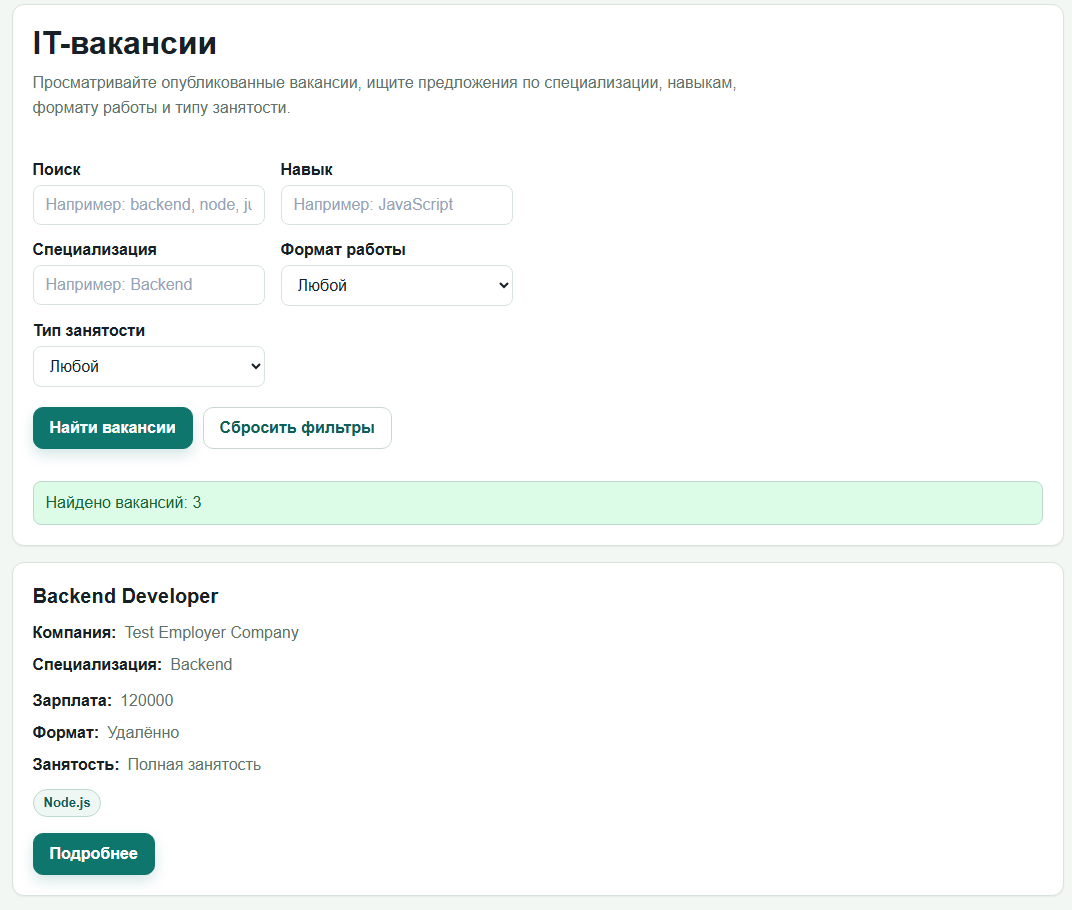
\includegraphics[width=\linewidth]{vacancies_list}
	\caption{Страница списка вакансий}
	\label{fig:vacancies-list}
\end{figure}

Как показано на рисунке~\ref{fig:vacancies-list}, страница списка вакансий содержит заголовок раздела, блок фильтрации, сведения о количестве найденных вакансий и список доступных предложений.

Для соискателя интерфейс должен обеспечивать доступ к просмотру и редактированию профиля, управлению навыками, просмотру вакансий, просмотру карточки вакансии, отправке откликов, просмотру своих откликов, а также к просмотру и управлению избранными вакансиями. Внешний вид страницы карточки вакансии представлен на рисунке~\ref{fig:vacancy-card}.

\begin{figure}[H]
	\centering
	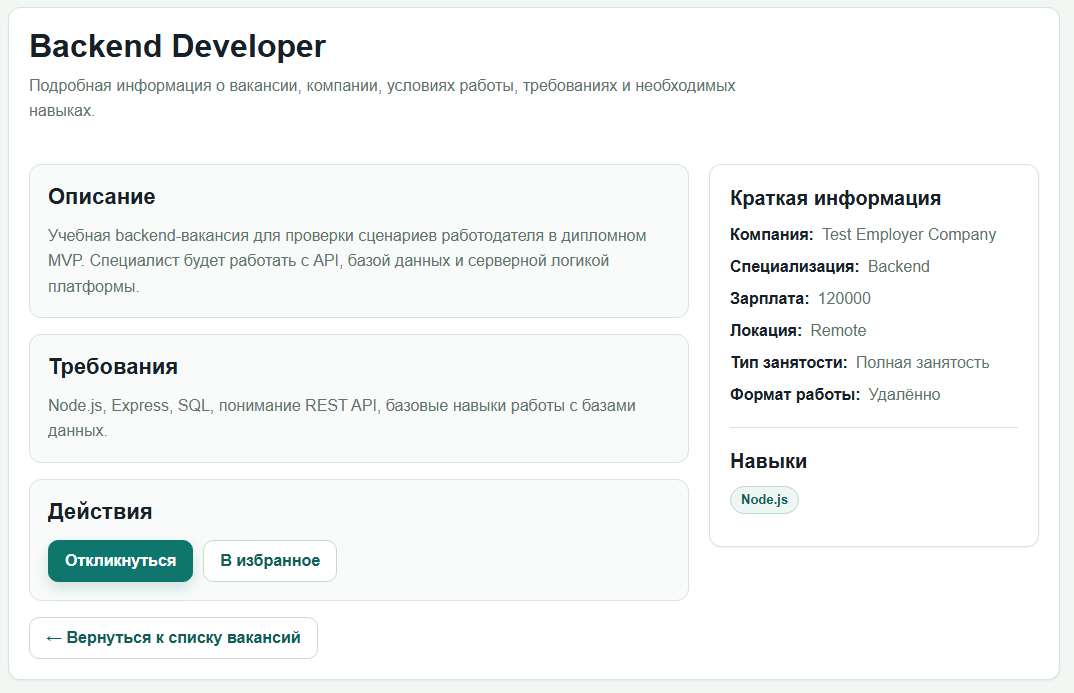
\includegraphics[width=\linewidth]{vacancy_card}
	\caption{Страница карточки вакансии}
	\label{fig:vacancy-card}
\end{figure}

Как показано на рисунке~\ref{fig:vacancy-card}, страница карточки вакансии содержит подробную информацию о выбранной вакансии, требованиях к кандидату, навыках и доступных действиях со стороны пользователя.

Для работодателя интерфейс должен обеспечивать доступ к просмотру и редактированию данных компании, созданию и редактированию вакансий, управлению публикацией вакансий, управлению навыками вакансии, просмотру откликов и фильтрации профилей соискателей. Внешний вид страницы работодателя со списком вакансий представлен на рисунке~\ref{fig:employer-vacancies}.

\begin{figure}[H]
	\centering
	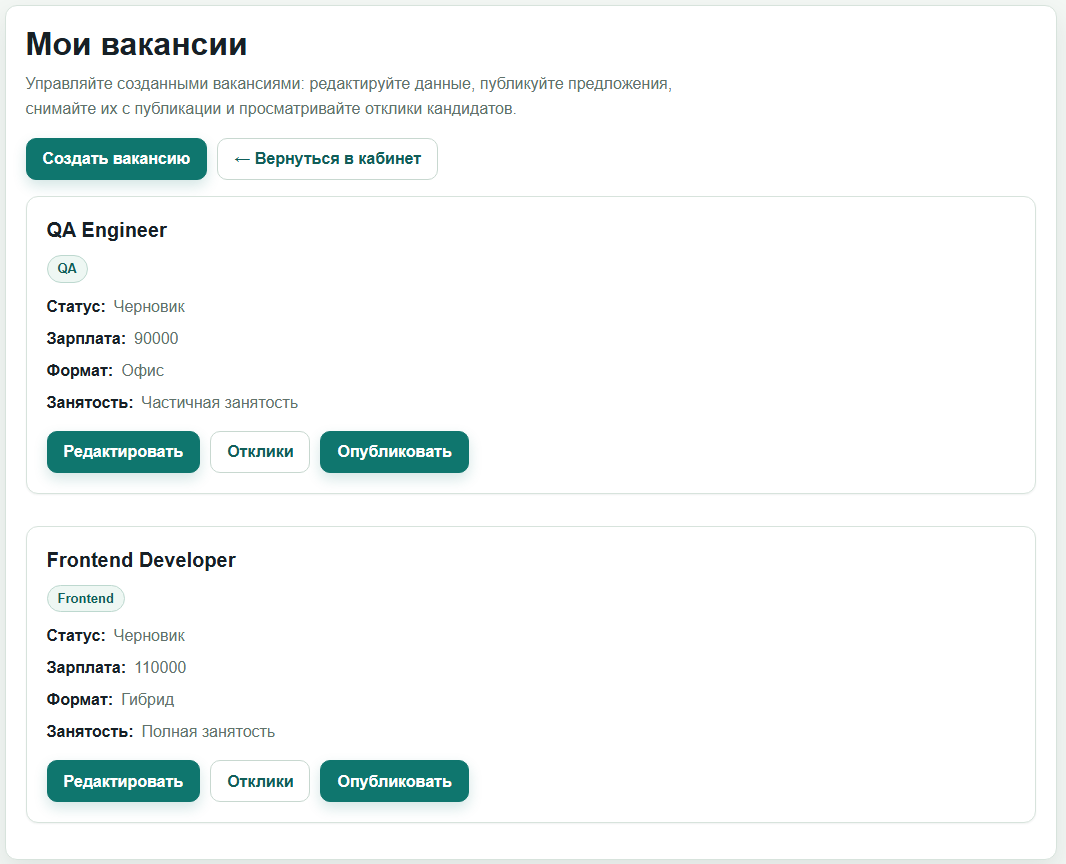
\includegraphics[width=\linewidth]{employer_vacancies}
	\caption{Страница работодателя со списком вакансий}
	\label{fig:employer-vacancies}
\end{figure}

Как показано на рисунке~\ref{fig:employer-vacancies}, страница работодателя содержит список созданных вакансий, сведения об их параметрах и элементы управления, связанные с редактированием, публикацией и просмотром откликов.

Для администратора интерфейс должен обеспечивать доступ к просмотру пользователей, просмотру вакансий, блокировке пользователей, снятию вакансий с публикации и удалению вакансий.

Интерфейс программной системы должен обеспечивать логичную навигацию между страницами, отображение результатов пользовательских действий, отображение сообщений об ошибках при некорректном вводе данных или попытке выполнения недопустимых действий, а также разграничение доступных элементов интерфейса в зависимости от роли пользователя.

\subsubsection{Требования к надёжности}

Программная система должна обеспечивать корректную обработку пользовательских действий и сохранение целостности данных при выполнении основных операций.

При вводе некорректных, неполных или недопустимых данных система должна предотвращать выполнение ошибочных операций и выводить пользователю сообщение об ошибке.

Система должна обеспечивать сохранение согласованности данных при работе с пользователями, профилями соискателей, компаниями, вакансиями, откликами, избранными вакансиями и навыками.

Система не должна допускать выполнение действий, нарушающих установленные ограничения предметной области, включая повторную отправку отклика на одну и ту же вакансию одним и тем же профилем соискателя, повторное добавление одной и той же вакансии в избранное одним и тем же пользователем, а также выполнение действий, не соответствующих роли пользователя.

При выполнении операций изменения данных система должна обеспечивать корректную обработку статусов вакансий и откликов, а также сохранение связей между сущностями программной системы.

В случае возникновения ошибок при обработке запроса система должна завершать операцию без нарушения целостности хранимых данных.

\subsubsection{Требования к информационной безопасности}

Программная система должна обеспечивать защиту данных пользователей и разграничение доступа к функциям и данным в зависимости от роли пользователя.

Доступ к функциям, связанным с изменением данных, должен предоставляться только авторизованным пользователям. Аутентификация пользователей должна выполняться на основе пары электронная почта и пароль.

Пароли пользователей не должны храниться в открытом виде и должны сохраняться в системе в виде хэша.

Авторизация пользователей в программной системе должна осуществляться с использованием JWT-токенов.

Программная система должна обеспечивать разграничение прав доступа между соискателем, работодателем и администратором. Пользователь не должен иметь возможность выполнять действия и получать доступ к данным, не предусмотренным его ролью.

Система должна ограничивать доступ пользователя к изменению только тех данных, которые относятся к его собственной учётной записи, профилю, компании, вакансиям, откликам и иным связанным объектам в пределах предоставленных прав.

Для пользователей, имеющих признак блокировки, должен быть запрещён доступ к использованию функциональных возможностей системы.

\subsubsection{Требования к программной и технической совместимости}

Программная система должна функционировать как web-приложение, доступ к которому осуществляется через web-интерфейс.

Серверная часть программной системы должна быть реализована с использованием Node.js и Express. Клиентская часть должна быть реализована на HTML, CSS и JavaScript без использования отдельного frontend-приложения.

Для хранения данных в системе должна использоваться система управления базами данных PostgreSQL.

Программная система должна поддерживать работу в монолитной клиент-серверной архитектуре, в которой серверное приложение одновременно обеспечивает обработку запросов, бизнес-логику и выдачу страниц пользовательского интерфейса.

Для развёртывания и запуска программной системы должно использоваться контейнерное окружение Docker.

Программная система предназначена для использования на персональном компьютере и не предполагает отдельной мобильной версии или мобильного приложения.

\subsection{Варианты использования программы}

Для разрабатываемой программной системы выделяются следующие акторы: гость, соискатель, работодатель и администратор.

Диаграммы прецедентов, отражающие взаимодействие указанных акторов с программной системой, представлены на рисунках~\ref{fig:guest-usecase}--\ref{fig:admin-usecase}.

На диаграммах представлены основные действия пользователей, связанные с просмотром вакансий, работой с профилем соискателя, размещением вакансий, обработкой откликов и выполнением административных функций.

\begin{figure}[H]
	\centering
	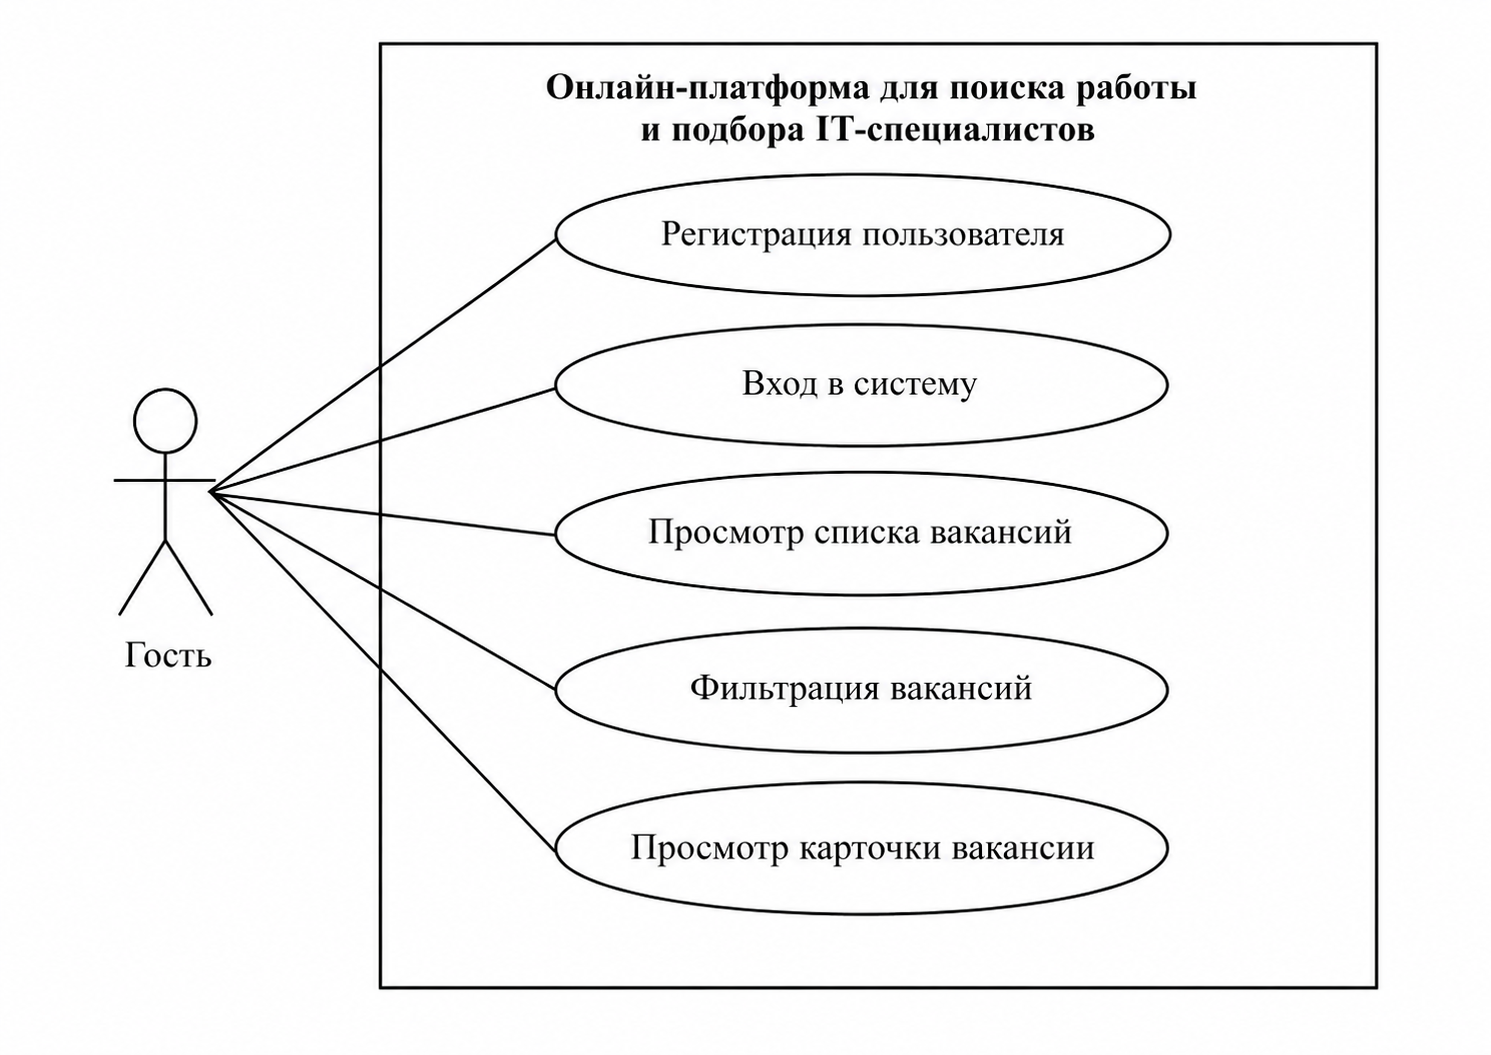
\includegraphics[width=0.88\linewidth]{guest_usecase}
	\caption{Диаграмма прецедентов для актора «Гость»}
	\label{fig:guest-usecase}
\end{figure}

\begin{figure}[H]
	\centering
	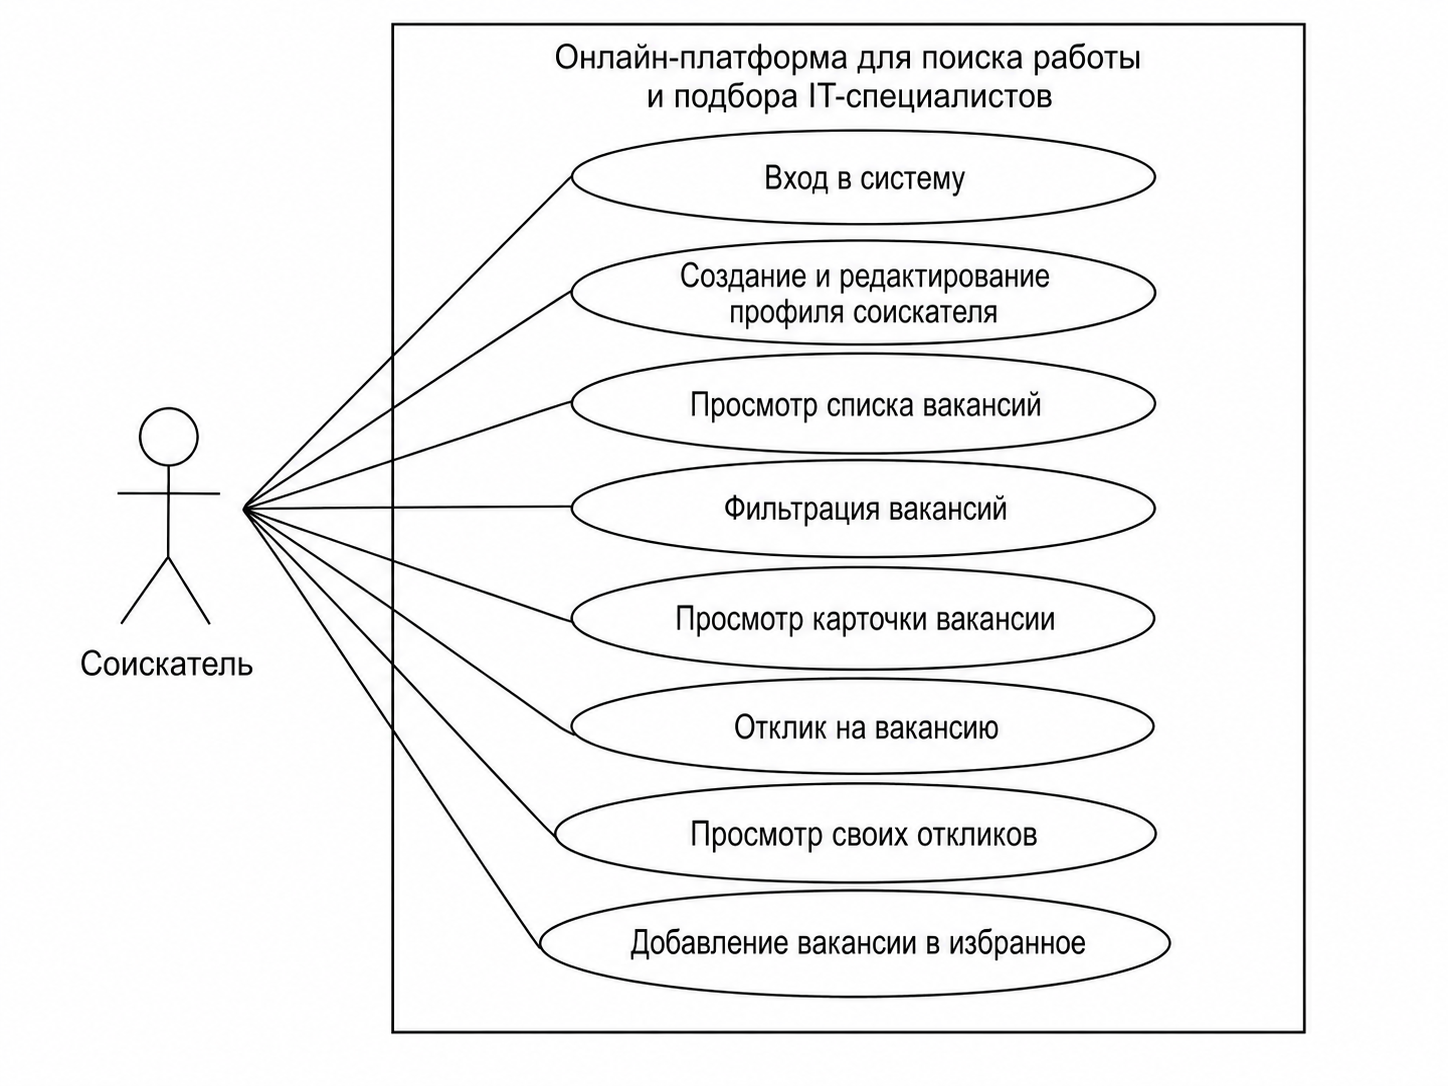
\includegraphics[width=0.88\linewidth]{jobseeker_usecase}
	\caption{Диаграмма прецедентов для актора «Соискатель»}
	\label{fig:jobseeker-usecase}
\end{figure}

\begin{figure}[H]
	\centering
	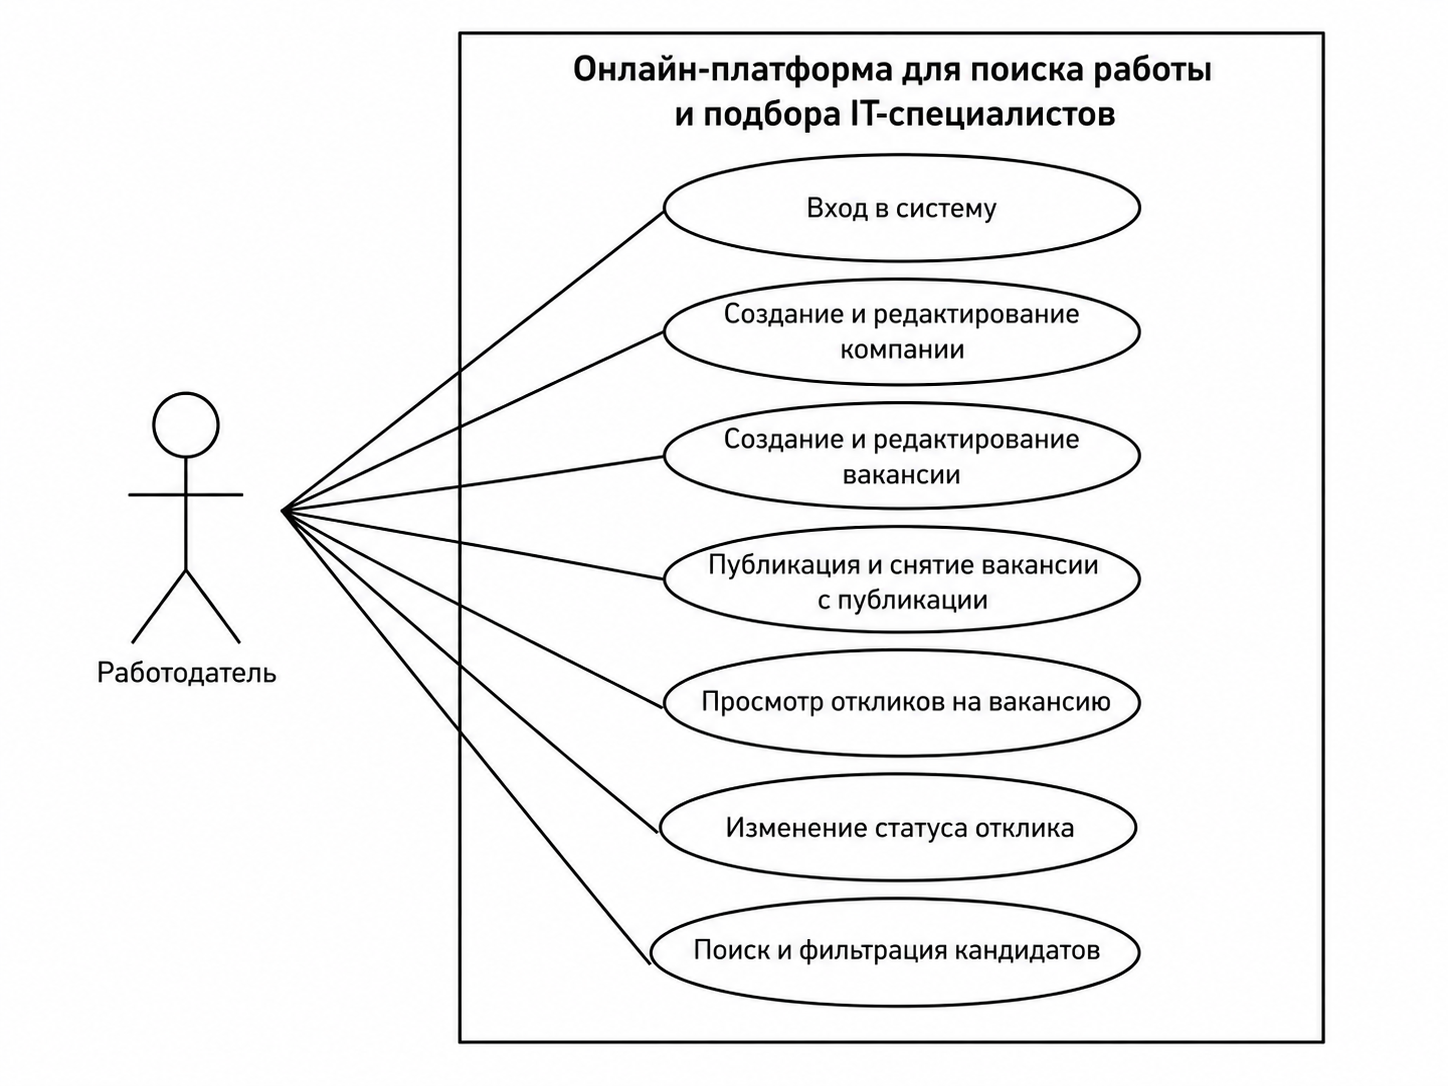
\includegraphics[width=0.88\linewidth]{employer_usecase}
	\caption{Диаграмма прецедентов для актора «Работодатель»}
	\label{fig:employer-usecase}
\end{figure}

\begin{figure}[H]
	\centering
	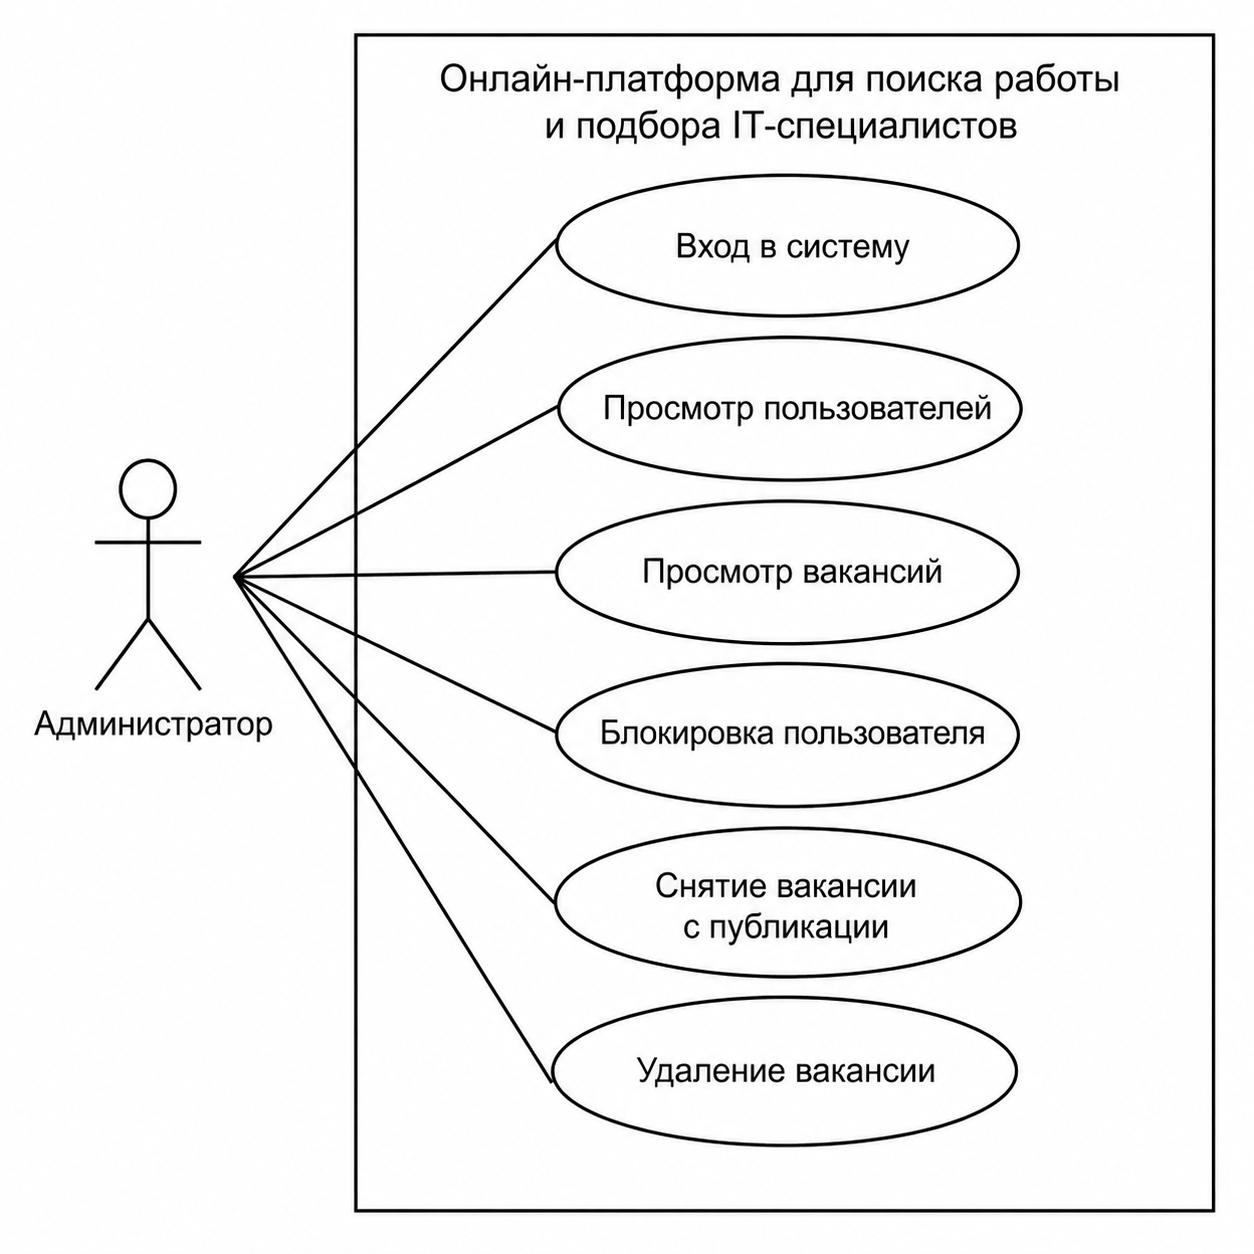
\includegraphics[width=0.77\linewidth]{admin_usecase}
	\caption{Диаграмма прецедентов для актора «Администратор»}
	\label{fig:admin-usecase}
\end{figure}

\subsubsection{Вариант использования «Регистрация пользователя»}

\textbf{Заинтересованное лицо:} неавторизованный пользователь.

\textbf{Предусловие:} пользователь открыл страницу регистрации в программной системе.

\textbf{Постусловие:} в системе создана новая учетная запись пользователя с ролью соискателя или работодателя.

\textbf{Основной сценарий:}
\begin{enumerate}
	\item Пользователь переходит на страницу регистрации.
	\item Пользователь вводит регистрационные данные.
	\item Пользователь выбирает роль соискателя или работодателя.
	\item Система выполняет проверку корректности введенных данных.
	\item Система создает новую учетную запись пользователя.
	\item Система сохраняет данные пользователя в базе данных.
\end{enumerate}

\textbf{Альтернативный сценарий:}
\begin{enumerate}
	\item Пользователь вводит некорректные, неполные или уже использованные регистрационные данные.
	\item Система не выполняет регистрацию пользователя.
	\item Система выводит сообщение об ошибке.
\end{enumerate}

\subsubsection{Вариант использования «Вход в систему»}

\textbf{Заинтересованное лицо:} пользователь.

\textbf{Предусловие:} пользователь имеет учетную запись в программной системе и открыл страницу входа.

\textbf{Постусловие:} пользователь авторизован в системе и получает доступ к функциям, предусмотренным его ролью.

\textbf{Основной сценарий:}
\begin{enumerate}
	\item Пользователь переходит на страницу входа.
	\item Пользователь вводит адрес электронной почты и пароль.
	\item Пользователь отправляет форму входа.
	\item Система проверяет корректность введенных учетных данных.
	\item Система выполняет авторизацию пользователя.
	\item Пользователь получает доступ к функциям системы в соответствии со своей ролью.
\end{enumerate}

\textbf{Альтернативный сценарий:}
\begin{enumerate}
	\item Пользователь вводит неверные учетные данные или оставляет обязательные поля незаполненными.
	\item Система не выполняет авторизацию пользователя.
	\item Система выводит сообщение об ошибке.
\end{enumerate}

\subsubsection{Вариант использования «Создание и редактирование профиля соискателя»}

\textbf{Заинтересованное лицо:} соискатель.

\textbf{Предусловие:} пользователь авторизован в системе с ролью соискателя.

\textbf{Постусловие:} профиль соискателя создан или обновлен.

\textbf{Основной сценарий:}
\begin{enumerate}
	\item Соискатель переходит к странице профиля.
	\item Соискатель вводит или изменяет данные профиля.
	\item Соискатель сохраняет внесенные изменения.
	\item Система проверяет корректность введенных данных.
	\item Система создает профиль соискателя или обновляет ранее сохраненные данные.
	\item Система сохраняет изменения в базе данных.
\end{enumerate}

\textbf{Альтернативный сценарий:}
\begin{enumerate}
	\item Соискатель вводит некорректные или неполные данные.
	\item Система не сохраняет изменения профиля.
	\item Система выводит сообщение об ошибке.
\end{enumerate}

\subsubsection{Вариант использования «Просмотр списка вакансий»}

\textbf{Заинтересованное лицо:} пользователь.

\textbf{Предусловие:} пользователь открыл страницу со списком вакансий.

\textbf{Постусловие:} пользователю отображен список опубликованных вакансий.

\textbf{Основной сценарий:}
\begin{enumerate}
	\item Пользователь переходит к странице со списком вакансий.
	\item Система получает данные об опубликованных вакансиях.
	\item Система формирует список вакансий.
	\item Система отображает пользователю список опубликованных вакансий.
\end{enumerate}

\textbf{Альтернативный сценарий:}
\begin{enumerate}
	\item В системе отсутствуют опубликованные вакансии.
	\item Система отображает пользователю сообщение об отсутствии доступных вакансий.
\end{enumerate}


\subsubsection{Вариант использования «Поиск и фильтрация вакансий»}

\textbf{Заинтересованное лицо:} пользователь.

\textbf{Предусловие:} пользователь открыл страницу со списком вакансий.

\textbf{Постусловие:} пользователю отображен список вакансий, соответствующих заданным параметрам фильтрации.

\textbf{Основной сценарий:}
\begin{enumerate}
	\item Пользователь переходит к странице со списком вакансий.
	\item Пользователь задает параметры фильтрации вакансий.
	\item Пользователь применяет выбранные параметры.
	\item Система получает параметры фильтрации.
	\item Система выполняет отбор вакансий, соответствующих заданным условиям.
	\item Система отображает пользователю обновленный список вакансий.
\end{enumerate}

\textbf{Альтернативный сценарий:}
\begin{enumerate}
	\item По заданным параметрам не найдено ни одной вакансии.
	\item Система отображает пользователю сообщение об отсутствии подходящих вакансий.
\end{enumerate}

\subsubsection{Вариант использования «Просмотр карточки вакансии»}

\textbf{Заинтересованное лицо:} пользователь.

\textbf{Предусловие:} пользователь открыл список вакансий или перешел по ссылке на конкретную вакансию.

\textbf{Постусловие:} пользователю отображена подробная информация о выбранной вакансии.

\textbf{Основной сценарий:}
\begin{enumerate}
	\item Пользователь выбирает вакансию из списка или переходит по ссылке на нее.
	\item Система получает данные о выбранной вакансии.
	\item Система формирует карточку вакансии.
	\item Система отображает пользователю подробную информацию о вакансии.
\end{enumerate}

\textbf{Альтернативный сценарий:}
\begin{enumerate}
	\item Выбранная вакансия отсутствует или недоступна для просмотра.
	\item Система не отображает карточку вакансии.
	\item Система выводит сообщение об ошибке.
\end{enumerate}

\subsubsection{Вариант использования «Отклик на вакансию»}

\textbf{Заинтересованное лицо:} соискатель.

\textbf{Предусловие:} пользователь авторизован в системе с ролью соискателя, имеет профиль соискателя и открыл карточку вакансии.

\textbf{Постусловие:} в системе создан новый отклик на выбранную вакансию.

\textbf{Основной сценарий:}
\begin{enumerate}
	\item Соискатель открывает карточку вакансии.
	\item Соискатель инициирует отправку отклика на вакансию.
	\item Система проверяет возможность создания отклика.
	\item Система создает новый отклик, связывающий профиль соискателя и выбранную вакансию.
	\item Система сохраняет отклик в базе данных.
	\item Система отображает результат успешной отправки отклика.
\end{enumerate}

\textbf{Альтернативный сценарий:}
\begin{enumerate}
	\item Соискатель уже отправлял отклик на выбранную вакансию либо выполнение операции невозможно.
	\item Система не создает новый отклик.
	\item Система выводит сообщение об ошибке.
\end{enumerate}

\subsubsection{Вариант использования «Просмотр своих откликов»}

\textbf{Заинтересованное лицо:} соискатель.

\textbf{Предусловие:} пользователь авторизован в системе с ролью соискателя.

\textbf{Постусловие:} соискателю отображен список ранее отправленных откликов с информацией об их статусах.

\textbf{Основной сценарий:}
\begin{enumerate}
	\item Соискатель переходит к разделу просмотра своих откликов.
	\item Система получает данные об откликах, связанных с профилем соискателя.
	\item Система формирует список откликов.
	\item Система отображает соискателю список его откликов и текущие статусы их обработки.
\end{enumerate}

\textbf{Альтернативный сценарий:}
\begin{enumerate}
	\item У соискателя отсутствуют ранее отправленные отклики.
	\item Система отображает сообщение об отсутствии откликов.
\end{enumerate}

\subsubsection{Вариант использования «Добавление вакансии в избранное»}

\textbf{Заинтересованное лицо:} соискатель.

\textbf{Предусловие:} пользователь авторизован в системе с ролью соискателя и открыл список вакансий или карточку вакансии.

\textbf{Постусловие:} выбранная вакансия добавлена в список избранных вакансий пользователя.

\textbf{Основной сценарий:}
\begin{enumerate}
	\item Соискатель открывает список вакансий или карточку вакансии.
	\item Соискатель инициирует добавление вакансии в избранное.
	\item Система проверяет возможность выполнения операции.
	\item Система добавляет выбранную вакансию в список избранных вакансий пользователя.
	\item Система сохраняет изменения в базе данных.
	\item Система отображает результат успешного выполнения операции.
\end{enumerate}

\textbf{Альтернативный сценарий:}
\begin{enumerate}
	\item Вакансия уже была ранее добавлена в избранное либо выполнение операции невозможно.
	\item Система не добавляет вакансию повторно.
	\item Система выводит сообщение об ошибке.
\end{enumerate}

\subsubsection{Вариант использования «Создание и редактирование компании»}

\textbf{Заинтересованное лицо:} работодатель.

\textbf{Предусловие:} пользователь авторизован в системе с ролью работодателя.

\textbf{Постусловие:} данные компании созданы или обновлены.

\textbf{Основной сценарий:}
\begin{enumerate}
	\item Работодатель переходит к разделу работы с данными компании.
	\item Работодатель вводит или изменяет данные компании.
	\item Работодатель сохраняет внесенные изменения.
	\item Система проверяет корректность введенных данных.
	\item Система создает данные компании или обновляет ранее сохраненные данные.
	\item Система сохраняет изменения в базе данных.
\end{enumerate}

\textbf{Альтернативный сценарий:}
\begin{enumerate}
	\item Работодатель вводит некорректные или неполные данные.
	\item Система не сохраняет изменения.
	\item Система выводит сообщение об ошибке.
\end{enumerate}

\subsubsection{Вариант использования «Создание и редактирование вакансии»}

\textbf{Заинтересованное лицо:} работодатель.

\textbf{Предусловие:} пользователь авторизован в системе с ролью работодателя и имеет созданные данные компании.

\textbf{Постусловие:} вакансия создана или обновлена.

\textbf{Основной сценарий:}
\begin{enumerate}
	\item Работодатель переходит к разделу работы с вакансиями.
	\item Работодатель инициирует создание новой вакансии или выбирает ранее созданную вакансию для редактирования.
	\item Работодатель вводит или изменяет данные вакансии.
	\item Работодатель сохраняет внесенные изменения.
	\item Система проверяет корректность введенных данных.
	\item Система создает новую вакансию или обновляет ранее сохраненные данные вакансии.
	\item Система сохраняет изменения в базе данных.
\end{enumerate}

\textbf{Альтернативный сценарий:}
\begin{enumerate}
	\item Работодатель вводит некорректные или неполные данные вакансии.
	\item Система не сохраняет изменения.
	\item Система выводит сообщение об ошибке.
\end{enumerate}

\subsubsection{Вариант использования «Публикация и снятие вакансии с публикации»}

\textbf{Заинтересованное лицо:} работодатель.

\textbf{Предусловие:} пользователь авторизован в системе с ролью работодателя и имеет ранее созданную вакансию.

\textbf{Постусловие:} статус вакансии изменен, в результате чего вакансия становится опубликованной или снимается с публикации.

\textbf{Основной сценарий:}
\begin{enumerate}
	\item Работодатель переходит к списку своих вакансий.
	\item Работодатель выбирает вакансию, для которой необходимо изменить статус публикации.
	\item Работодатель инициирует публикацию вакансии или снятие ее с публикации.
	\item Система проверяет возможность выполнения операции.
	\item Система изменяет статус вакансии.
	\item Система сохраняет изменения в базе данных.
	\item Система отображает результат успешного выполнения операции.
\end{enumerate}

\textbf{Альтернативный сценарий:}
\begin{enumerate}
	\item Выполнение операции публикации или снятия вакансии с публикации невозможно.
	\item Система не изменяет статус вакансии.
	\item Система выводит сообщение об ошибке.
\end{enumerate}

\subsubsection{Вариант использования «Просмотр откликов на вакансию»}

\textbf{Заинтересованное лицо:} работодатель.

\textbf{Предусловие:} пользователь авторизован в системе с ролью работодателя и открыл раздел просмотра откликов по выбранной вакансии.

\textbf{Постусловие:} работодателю отображен список откликов, связанных с выбранной вакансией.

\textbf{Основной сценарий:}
\begin{enumerate}
	\item Работодатель переходит к списку своих вакансий.
	\item Работодатель выбирает вакансию, для которой необходимо просмотреть отклики.
	\item Система получает данные об откликах, связанных с выбранной вакансией.
	\item Система формирует список откликов.
	\item Система отображает работодателю список откликов по выбранной вакансии.
\end{enumerate}

\textbf{Альтернативный сценарий:}
\begin{enumerate}
	\item Для выбранной вакансии отсутствуют отклики.
	\item Система отображает сообщение об отсутствии откликов.
\end{enumerate}

\subsubsection{Вариант использования «Изменение статуса отклика»}

\textbf{Заинтересованное лицо:} работодатель.

\textbf{Предусловие:} пользователь авторизован в системе с ролью работодателя и открыл список откликов на свою вакансию.

\textbf{Постусловие:} статус выбранного отклика изменен и сохранен в системе.

\textbf{Основной сценарий:}
\begin{enumerate}
	\item Работодатель переходит к списку откликов на выбранную вакансию.
	\item Работодатель выбирает отклик, статус которого необходимо изменить.
	\item Работодатель задает новый статус отклика.
	\item Система проверяет возможность выполнения операции.
	\item Система изменяет статус выбранного отклика.
	\item Система сохраняет изменения в базе данных.
	\item Система отображает результат успешного выполнения операции.
\end{enumerate}

\textbf{Альтернативный сценарий:}
\begin{enumerate}
	\item Изменение статуса отклика невозможно.
	\item Система не сохраняет изменения.
	\item Система выводит сообщение об ошибке.
\end{enumerate}

\subsubsection{Вариант использования «Поиск и фильтрация кандидатов»}

\textbf{Заинтересованное лицо:} работодатель.

\textbf{Предусловие:} пользователь авторизован в системе с ролью работодателя и открыл раздел просмотра профилей соискателей.

\textbf{Постусловие:} работодателю отображен список профилей соискателей, соответствующих заданным параметрам отбора.

\textbf{Основной сценарий:}
\begin{enumerate}
	\item Работодатель переходит к разделу просмотра профилей соискателей.
	\item Работодатель задает параметры отбора кандидатов.
	\item Работодатель применяет выбранные параметры.
	\item Система получает параметры отбора.
	\item Система выполняет отбор профилей соискателей, соответствующих заданным условиям.
	\item Система отображает работодателю список подходящих профилей соискателей.
\end{enumerate}

\textbf{Альтернативный сценарий:}
\begin{enumerate}
	\item По заданным параметрам не найдено ни одного подходящего профиля соискателя.
	\item Система отображает сообщение об отсутствии подходящих кандидатов.
\end{enumerate}

\subsubsection{Вариант использования «Просмотр пользователей администратором»}

\textbf{Заинтересованное лицо:} администратор.

\textbf{Предусловие:} пользователь авторизован в системе с ролью администратора.

\textbf{Постусловие:} администратору отображен список пользователей программной системы.

\textbf{Основной сценарий:}
\begin{enumerate}
	\item Администратор переходит к разделу просмотра пользователей.
	\item Система получает данные о зарегистрированных пользователях.
	\item Система формирует список пользователей.
	\item Система отображает администратору список пользователей программной системы.
\end{enumerate}

\textbf{Альтернативный сценарий:}
\begin{enumerate}
	\item В системе отсутствуют зарегистрированные пользователи.
	\item Система отображает сообщение об отсутствии пользователей.
\end{enumerate}

\subsubsection{Вариант использования «Просмотр вакансий администратором»}

\textbf{Заинтересованное лицо:} администратор.

\textbf{Предусловие:} пользователь авторизован в системе с ролью администратора.

\textbf{Постусловие:} администратору отображен список вакансий программной системы.

\textbf{Основной сценарий:}
\begin{enumerate}
	\item Администратор переходит к разделу просмотра вакансий.
	\item Система получает данные о вакансиях программной системы.
	\item Система формирует список вакансий.
	\item Система отображает администратору список вакансий.
\end{enumerate}

\textbf{Альтернативный сценарий:}
\begin{enumerate}
	\item В системе отсутствуют вакансии.
	\item Система отображает сообщение об отсутствии вакансий.
\end{enumerate}

\subsubsection{Вариант использования «Блокировка пользователя»}

\textbf{Заинтересованное лицо:} администратор.

\textbf{Предусловие:} пользователь авторизован в системе с ролью администратора и открыл список пользователей.

\textbf{Постусловие:} выбранный пользователь заблокирован в системе.

\textbf{Основной сценарий:}
\begin{enumerate}
	\item Администратор переходит к разделу просмотра пользователей.
	\item Администратор выбирает пользователя, которого необходимо заблокировать.
	\item Администратор инициирует блокировку пользователя.
	\item Система проверяет возможность выполнения операции.
	\item Система изменяет состояние выбранного пользователя на заблокированное.
	\item Система сохраняет изменения в базе данных.
	\item Система отображает результат успешного выполнения операции.
\end{enumerate}

\textbf{Альтернативный сценарий:}
\begin{enumerate}
	\item Выполнение операции блокировки невозможно.
	\item Система не изменяет состояние пользователя.
	\item Система выводит сообщение об ошибке.
\end{enumerate}

\subsubsection{Вариант использования «Снятие вакансии с публикации администратором»}

\textbf{Заинтересованное лицо:} администратор.

\textbf{Предусловие:} пользователь авторизован в системе с ролью администратора и открыл список вакансий.

\textbf{Постусловие:} выбранная вакансия снята с публикации.

\textbf{Основной сценарий:}
\begin{enumerate}
	\item Администратор переходит к разделу просмотра вакансий.
	\item Администратор выбирает вакансию, которую необходимо снять с публикации.
	\item Администратор инициирует снятие вакансии с публикации.
	\item Система проверяет возможность выполнения операции.
	\item Система изменяет статус выбранной вакансии.
	\item Система сохраняет изменения в базе данных.
	\item Система отображает результат успешного выполнения операции.
\end{enumerate}

\textbf{Альтернативный сценарий:}
\begin{enumerate}
	\item Выполнение операции снятия вакансии с публикации невозможно.
	\item Система не изменяет статус вакансии.
	\item Система выводит сообщение об ошибке.
\end{enumerate}

\subsubsection{Вариант использования «Удаление вакансии администратором»}

\textbf{Заинтересованное лицо:} администратор.

\textbf{Предусловие:} пользователь авторизован в системе с ролью администратора и открыл список вакансий.

\textbf{Постусловие:} выбранная вакансия удалена из системы.

\textbf{Основной сценарий:}
\begin{enumerate}
	\item Администратор переходит к разделу просмотра вакансий.
	\item Администратор выбирает вакансию, которую необходимо удалить.
	\item Администратор инициирует удаление вакансии.
	\item Система проверяет возможность выполнения операции.
	\item Система удаляет выбранную вакансию.
	\item Система сохраняет изменения в базе данных.
	\item Система отображает результат успешного выполнения операции.
\end{enumerate}

\textbf{Альтернативный сценарий:}
\begin{enumerate}
	\item Выполнение операции удаления вакансии невозможно.
	\item Система не удаляет вакансию.
	\item Система выводит сообщение об ошибке.
\end{enumerate}

\subsection{Требования к оформлению документации}

Программная документация и текст выпускной квалификационной работы должны оформляться в соответствии с требованиями, предъявляемыми к выпускным квалификационным работам по направлению 09.03.04 «Программная инженерия», методическими указаниями кафедры и действующими нормативными документами, регламентирующими оформление программной документации.

Схемы, диаграммы, таблицы, иллюстрации и иные графические материалы должны оформляться в соответствии с установленными требованиями к оформлению выпускной квалификационной работы.
\section{Технический проект}
\subsection{Архитектура программной системы}

Разрабатываемая программная система представляет собой клиент-серверную web-платформу, предназначенную для поиска IT-вакансий и подбора IT-специалистов. Выбор клиент-серверной архитектуры обусловлен необходимостью разграничения пользовательского интерфейса, серверной логики и подсистемы хранения данных, а также поддержкой работы нескольких категорий пользователей в рамках единой программной среды. В системе предусмотрены роли неавторизованного пользователя, соискателя, работодателя и администратора, каждая из которых взаимодействует с платформой в пределах доступных ей функций.

Клиентская часть системы функционирует в браузере и предоставляет пользователю набор web-страниц для просмотра вакансий, регистрации и авторизации, ведения профиля соискателя, управления компанией работодателя, работы с откликами, избранными вакансиями и административными разделами. Доступ к пользовательскому интерфейсу осуществляется через набор маршрутов, соответствующих основным страницам платформы. Логика отображения данных и выполнения пользовательских действий реализуется на стороне клиента средствами HTML, CSS и JavaScript.

Серверная часть системы реализована в виде единого приложения на платформе Node.js с использованием фреймворка Express. Она построена по модульному принципу: маршруты (routes/), контроллеры (controllers/), сервисы (services/), промежуточные обработчики (middlewares/) и модели данных (models/) выделены в отдельные компоненты, что упрощает сопровождение и развитие системы. Сервер обрабатывает HTTP-запросы, выполняет маршрутизацию, проверяет права доступа через соответствующие middleware, реализует бизнес-логику и обеспечивает взаимодействие с базой данных. На уровне серверной логики можно выделить основные функциональные подсистемы: аутентификацию и управление пользователями, работу с профилем соискателя, управление навыками, ведение данных о компании, размещение и публикацию вакансий, обработку откликов, управление избранными вакансиями, поиск кандидатов и административное управление. Обмен данными между клиентской и серверной частями осуществляется через REST API, размещённый по префиксу /api.

Аутентификация пользователей построена на использовании JWT-токенов: при успешном входе клиент получает токен, который затем передаётся в заголовке Authorization при каждом защищённом запросе. Проверка токена и извлечение роли пользователя выполняются в middleware auth.middleware.js и role.middleware.js, что позволяет централизованно разграничивать доступ к функциям системы.

Подсистема хранения данных построена на основе реляционной системы управления базами данных PostgreSQL. Взаимодействие с ней осуществляется через ORM Sequelize, что обеспечивает объектно-ориентированный доступ к данным, параметризацию запросов и защиту от SQL-инъекций. База данных предназначена для хранения сведений о пользователях, профилях соискателей, компаниях, вакансиях, откликах, избранных вакансиях и навыках. Такое разделение позволяет обеспечить структурированное хранение информации, связность данных и поддержку основных процессов платформы, связанных с публикацией вакансий, поиском кандидатов и рассмотрением откликов.

С точки зрения организации взаимодействия компонентов работа системы осуществляется следующим образом. Пользователь через браузер открывает соответствующую страницу платформы и инициирует действие, например просмотр списка вакансий, отправку отклика, редактирование профиля или создание вакансии. Клиентская часть формирует запрос к серверу; серверное приложение принимает его, выполняет необходимую обработку (включая проверку прав, валидацию и обращение к сервисному слою), при необходимости взаимодействует с базой данных и возвращает результат клиенту в формате JSON. После этого интерфейс обновляется с учётом полученного ответа. Такой подход обеспечивает централизованную обработку данных, упрощает сопровождение системы и позволяет разграничить ответственность между уровнями представления, прикладной логики и хранения данных.

Дополнительно архитектура системы предусматривает возможность контейнеризированного развёртывания. В составе окружения используются контейнер приложения и контейнер базы данных, взаимодействующие между собой в рамках конфигурации Docker Compose. Это упрощает запуск системы, изоляцию компонентов и воспроизводимость программной среды при разработке и тестировании. Общая схема архитектуры программной системы представлена на рисунке 3.1.

\begin{figure}[H]
	\centering
	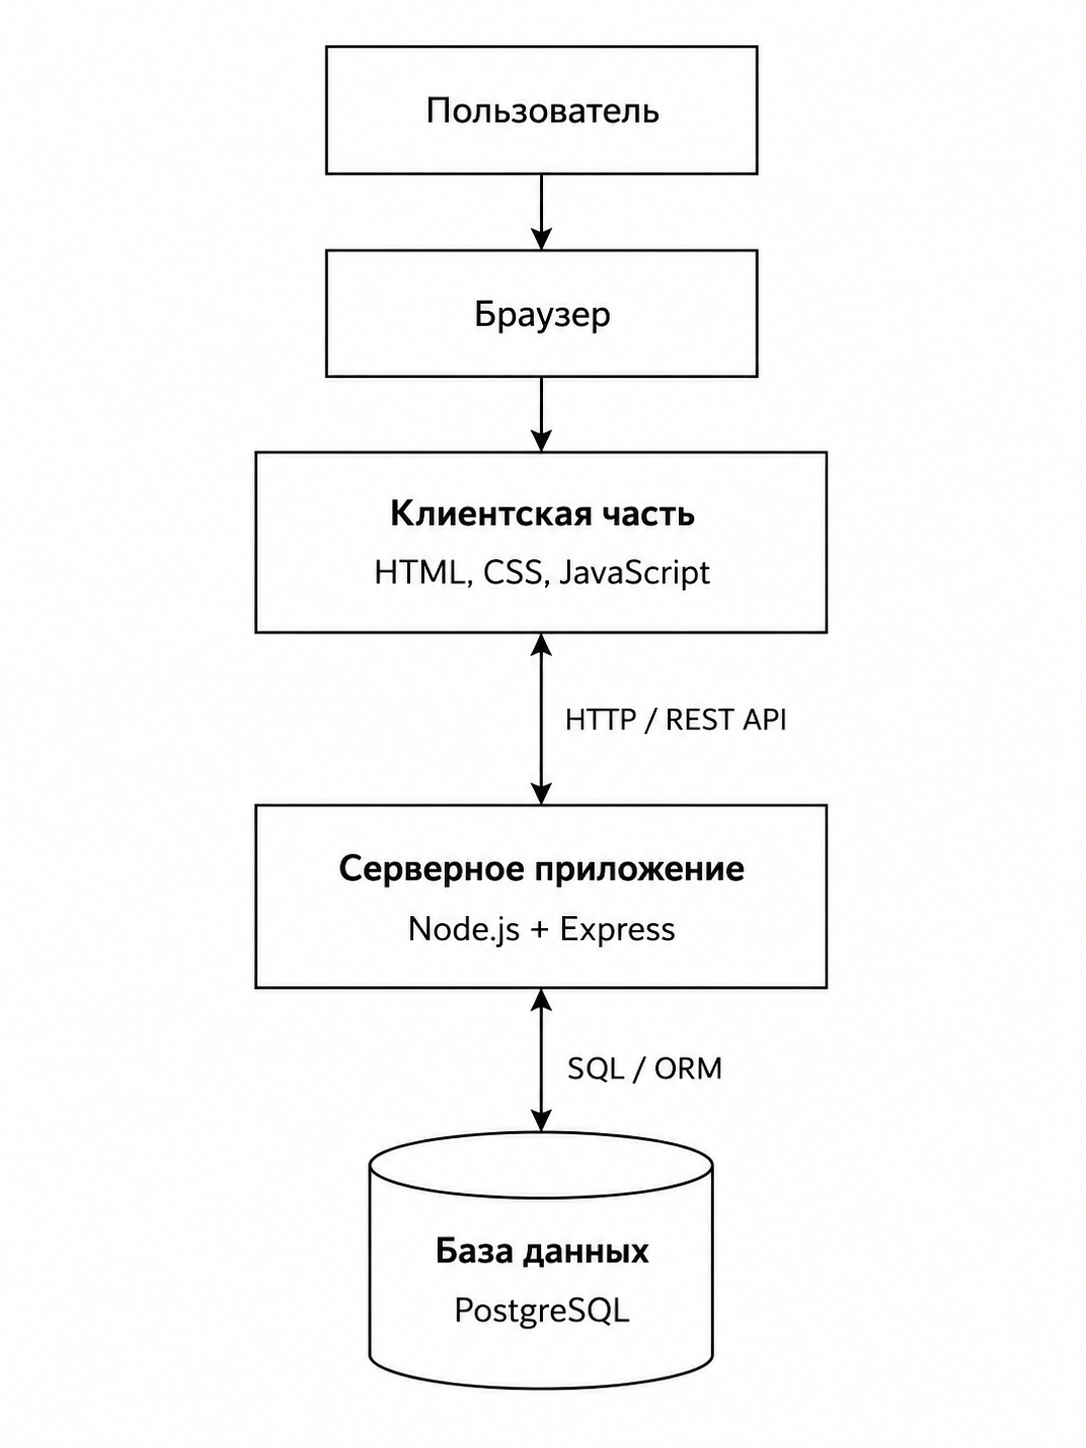
\includegraphics[width=0.70\linewidth]{fig_3_1_architecture.png}
	\caption{Архитектура программной системы}
	\label{fig:architecture}
\end{figure}

\subsection{Обоснование выбора технологий проектирования}

Выбор технологического стека для реализации платформы определялся архитектурой клиент-серверного web-приложения, необходимостью обеспечить надёжную обработку запросов, структурированное хранение данных, разграничение доступа пользователей и воспроизводимость программного окружения. В проекте используется стек, включающий Node.js, Express, PostgreSQL, Sequelize, JWT, bcryptjs, клиентские технологии HTML, CSS и JavaScript, а также Docker для контейнеризации среды выполнения.

В качестве серверной платформы выбрана Node.js. Это решение позволяет использовать JavaScript как на серверной, так и на клиентской стороне, что делает проект более однородным с точки зрения разработки и сопровождения. Для платформы это удобно, поскольку серверная часть реализует REST API, а клиентская часть построена на статических HTML-страницах с JavaScript-логикой, взаимодействующей с сервером через HTTP-запросы. Развитая экосистема npm также дала возможность применить необходимые библиотеки для маршрутизации, работы с базой данных, аутентификации и обработки cookie.

Веб-фреймворк Express использован для построения серверной части приложения. Он позволил организовать обработку HTTP-запросов, подключение middleware, раздачу статических файлов и маршрутизацию API по префиксу /api. В рамках проекта Express выступает основой единого серверного приложения, обслуживающего как клиентские страницы, так и программный интерфейс взаимодействия с данными платформы.

Для хранения данных выбрана система управления базами данных PostgreSQL. Данное решение подходит для платформы, в которой используются строго структурированные сущности и связи между ними: пользователи, профили соискателей, компании, вакансии, отклики, навыки и избранные вакансии. Применение реляционной СУБД позволяет обеспечить целостность данных, поддержку ограничений и надёжное хранение информации, задействованной в основных бизнес-процессах системы. Кроме того, PostgreSQL включена в состав контейнеризированного окружения проекта и запускается как отдельный сервис базы данных.

Для взаимодействия серверной части с базой данных применяется ORM Sequelize. Его использование позволило описывать модели и связи между ними на уровне приложения, управлять схемой базы данных через миграции и сократить объём рутинного кода при выполнении типовых операций чтения и записи. Для данного проекта это особенно важно из-за наличия нескольких связанных сущностей и промежуточных таблиц, обеспечивающих работу с навыками, откликами и избранными вакансиями.

Аутентификация пользователей реализована на основе механизма JWT. После успешного входа в систему сервер формирует токен, содержащий идентификатор пользователя, адрес электронной почты и его роль, после чего сохраняет этот токен в cookie. Дальнейшая проверка подлинности пользователя выполняется middleware серверной части, которое извлекает токен из cookie, проверяет его корректность и загружает сведения о текущем пользователе. Такой подход позволяет централизовать контроль доступа к защищённым маршрутам системы.

Для защиты паролей применяется библиотека bcryptjs. Перед сохранением в базе данных пароль преобразуется в хеш, что исключает хранение пользовательских паролей в открытом виде и повышает безопасность системы при работе с учётными записями.

Клиентская часть проекта реализована средствами HTML, CSS и JavaScript без использования дополнительных frontend-фреймворков. Такое решение соответствует структуре системы, в которой пользовательский интерфейс построен как набор отдельных страниц, каждая из которых отвечает за конкретный сценарий работы: просмотр вакансий, авторизацию, редактирование профиля, работу с откликами, управление вакансиями и административные действия. Отказ от отдельного frontend-фреймворка и этапа сборки упростил структуру проекта и сохранил достаточность клиентских средств для всех реализованных функций.

Для обеспечения единообразия программного окружения в проекте используется контейнеризация Docker. Конфигурация среды включает два основных сервиса: контейнер приложения и контейнер базы данных. Такой подход упрощает запуск системы, обеспечивает воспроизводимость окружения и изолирует основные компоненты платформы друг от друга.

Таким образом, выбранный технологический стек соответствует архитектуре разработанной платформы и обеспечивает реализацию серверной логики, клиентского интерфейса, хранения данных, аутентификации пользователей и контейнеризированного развёртывания системы.

\subsection{Клиентская часть}

Клиентская часть платформы представляет собой набор web-страниц, таблиц стилей CSS и клиентских JavaScript-скриптов, исполняемых в браузере пользователя. Серверная часть обеспечивает выдачу страниц и обработку API-запросов, а клиентская часть отвечает за отображение данных, обработку действий пользователя и динамическое обновление содержимого страниц.

Структура клиентской части организована в соответствии с основными пользовательскими ролями, предусмотренными в системе. Для неавторизованного пользователя доступны главная страница, страницы входа и регистрации, список опубликованных вакансий и карточка отдельной вакансии. На этих страницах реализованы просмотр опубликованных предложений, переход к подробной информации о вакансии и фильтрация вакансий по основным параметрам.

Интерфейс соискателя включает страницы ведения профиля, управления навыками, просмотра вакансий, отправки откликов, работы с избранными вакансиями и просмотра статусов ранее отправленных откликов. Через эти страницы соискатель может редактировать сведения о себе, управлять набором навыков, открывать карточки вакансий, отправлять отклики и отслеживать результаты взаимодействия с работодателями.

Интерфейс работодателя включает страницы управления данными компании, создания и редактирования вакансий, просмотра списка собственных вакансий, обработки откликов и поиска кандидатов. С помощью соответствующих форм работодатель может изменять сведения о компании, публиковать вакансии, снимать их с публикации, просматривать отклики, изменять их статус и выполнять поиск профилей соискателей по доступным параметрам.

Для администратора реализован отдельный интерфейс, предназначенный для просмотра пользователей и вакансий, а также выполнения административных действий. Через административные страницы обеспечиваются блокировка пользователей, снятие вакансий с публикации и удаление вакансий в пределах полномочий данной роли.

HTML-разметка страниц определяет структуру пользовательского интерфейса, включая формы ввода, списки объектов, карточки вакансий, элементы навигации и служебные блоки. Единое визуальное оформление страниц обеспечивается таблицами стилей CSS, размещёнными в каталоге public/css/. Использование общего набора стилей позволяет поддерживать единообразный внешний вид форм, карточек, списков и элементов управления во всех разделах платформы.

Динамическое поведение клиентской части реализуется с помощью JavaScript-скриптов, размещённых в каталоге public/js/. Они используются для загрузки данных с сервера через REST API, отправки данных форм, обработки ответов в формате JSON и изменения содержимого страниц в зависимости от результатов выполнения запроса. Такой подход позволяет отделить отображение данных в браузере от серверной бизнес-логики и обеспечить гибкое взаимодействие между пользовательским интерфейсом и серверной частью системы.

Обмен данными между клиентской и серверной частями осуществляется по модели «запрос–ответ». При выполнении пользовательского действия — открытии списка вакансий, сохранении профиля, создании вакансии или отправке отклика — клиентский скрипт формирует HTTP-запрос к соответствующему API-маршруту. Сервер обрабатывает запрос, выполняет необходимые операции и возвращает ответ, после чего интерфейс страницы обновляется в соответствии с полученными данными. Такой механизм позволяет реализовать интерактивное поведение страниц при сохранении общей простоты архитектуры клиентской части.

На стороне клиента также выполняется базовая проверка корректности вводимых данных перед их отправкой на сервер. При возникновении ошибки интерфейс отображает пользователю сообщение о невозможности выполнения операции, не раскрывая внутренние детали серверной реализации. Это повышает удобство работы с платформой и делает взаимодействие с системой более понятным для пользователя.

Таким образом, клиентская часть платформы обеспечивает реализацию всех пользовательских сценариев, связанных с просмотром вакансий, работой с профилем соискателя, управлением компанией и вакансиями, обработкой откликов и выполнением административных действий. Её структура соответствует ролевой модели системы и обеспечивает взаимодействие с серверной частью через REST API. Структура клиентской части и её взаимодействие с сервером представлены на рисунке 3.2.

\begin{figure}[H]
	\centering
	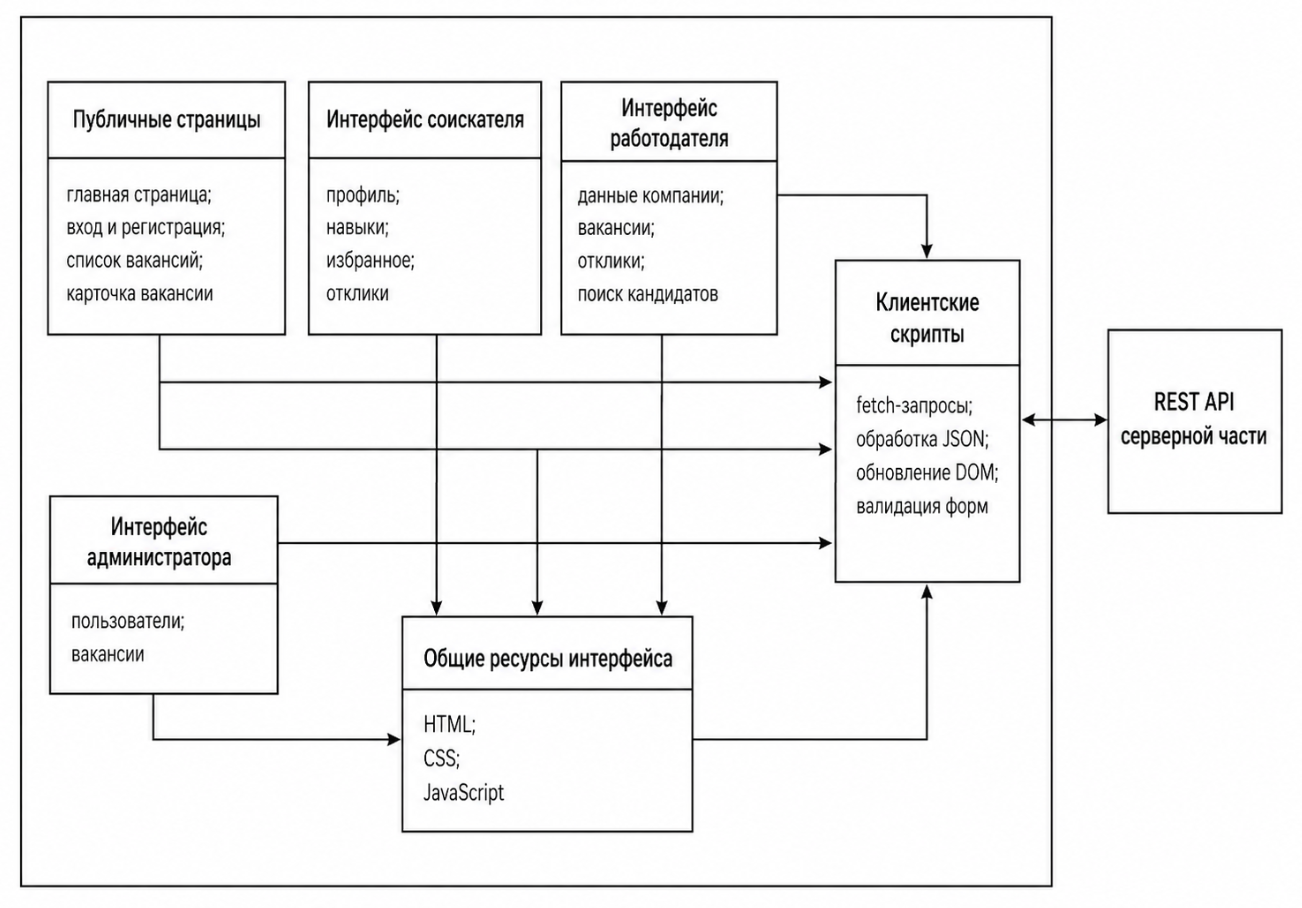
\includegraphics[width=0.79\linewidth]{fig_3_2_client_part.png}
	\caption{Структура клиентской части и её взаимодействие с сервером}
	\label{fig:client_part}
\end{figure}

\subsection{Серверная часть}

Серверная часть платформы построена по модульному принципу и включает маршруты API, промежуточные обработчики, контроллеры, сервисный слой и модели данных, взаимодействующие с базой данных PostgreSQL через ORM Sequelize. Структура серверной части представлена на рисунке 3.3.

\begin{figure}[H]
	\centering
	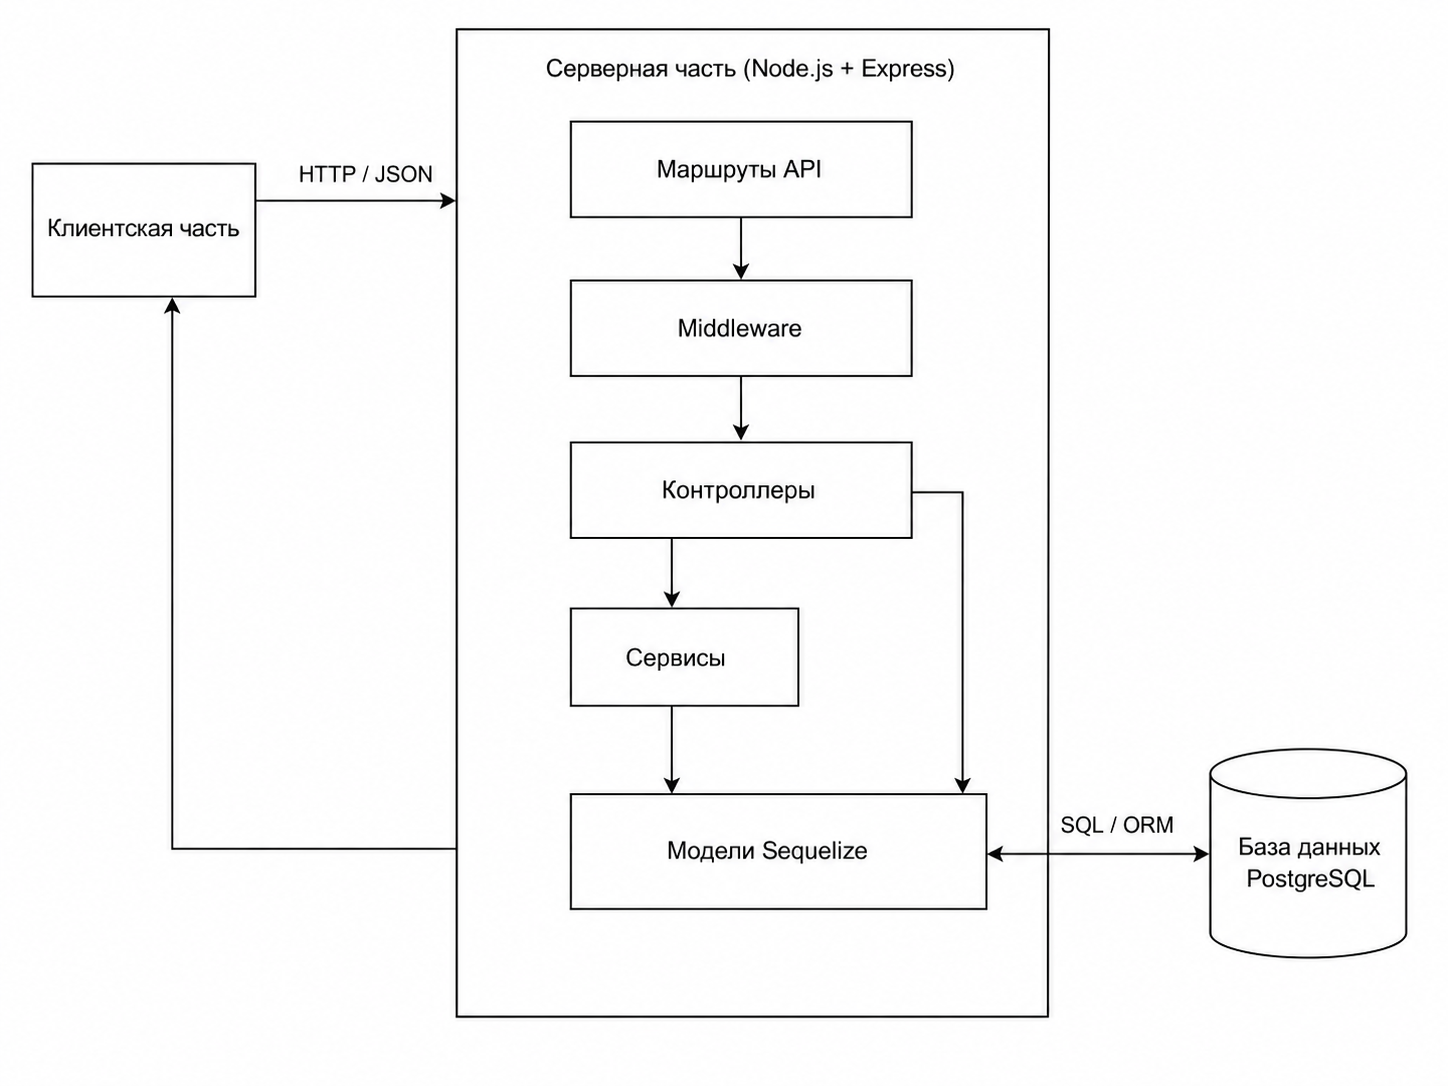
\includegraphics[width=\linewidth]{fig_3_3_server_part.png}
	\caption{Структура серверной части}
	\label{fig:server_part}
\end{figure}

Серверное приложение предоставляет REST API, через которое клиентская часть получает доступ к данным и выполняет основные операции программной системы. Маршруты API сгруппированы по функциональным подсистемам: аутентификация, работа с профилем соискателя, компанией, вакансиями, откликами, избранными вакансиями, навыками, пользовательскими и административными данными, а также приложения. Обмен данными между клиентской и серверной частями осуществляется в формате JSON. Доступ к части маршрутов открыт всем пользователям, тогда как операции, связанные с изменением данных и доступом к защищённым разделам системы, требуют аутентификации и, при необходимости, проверки роли пользователя. Далее приведено полное описание основных API-маршрутов программной системы с указанием их назначения, входных данных, структуры успешных JSON-ответов и основных ошибочных ситуаций.

\subsubsection{Служебный маршрут проверки работоспособности}

\textbf{Маршрут GET /api/health.}

Данный маршрут предназначен для проверки доступности серверного API. Он не требует аутентификации и может использоваться для контроля работоспособности серверной части приложения.

Path-параметры, query-параметры и тело запроса для данного маршрута отсутствуют.

При успешной обработке сервер возвращает ответ со статусом 200.

Пример успешного JSON-ответа:

\begin{flushleft}
	\small\ttfamily
	\{ "message": "API is working" \}
\end{flushleft}

Специальные бизнес-ошибки для данного маршрута не предусмотрены.

\subsubsection{Аутентификация}

Группа маршрутов аутентификации обеспечивает регистрацию пользователя, вход в систему, получение данных о текущем пользователе и завершение сессии. Основными маршрутами данной группы являются POST /api/auth/register, POST /api/auth/login, GET /api/auth/me и POST /api/auth/logout.

\textbf{Маршрут POST /api/auth/register.}

Маршрут предназначен для регистрации нового пользователя. Он доступен без предварительной аутентификации.

В теле запроса передаются поля email, password, fullName и role. Поле role может принимать только значения candidate или employer. Path-параметры и query-параметры отсутствуют.

При успешной регистрации сервер возвращает ответ со статусом 201 и JSON-объект, содержащий сообщение и краткие данные созданного пользователя.

Пример успешного JSON-ответа:

\begin{flushleft}
	\small\ttfamily
	\{ "message": "User registered successfully",\\
	"user": \{ "id": 1, "email": "candidate@example.com",\\
	"fullName": "Иван Иванов", "role": "candidate",\\
	"isBlocked": false \} \}
\end{flushleft}

Основные ошибки данного маршрута: 400 при отсутствии обязательных полей, недопустимой роли или попытке зарегистрировать уже существующий адрес электронной почты.

\textbf{Маршрут POST /api/auth/login.}

Маршрут предназначен для входа пользователя в систему. Он доступен без предварительной аутентификации.

В теле запроса передаются поля email и password. Path-параметры и query-параметры отсутствуют.

При успешной проверке учётных данных сервер возвращает ответ со статусом 200, формирует cookie token с JWT и передаёт JSON-объект с сообщением и краткими сведениями о пользователе.

Пример успешного JSON-ответа:

\begin{flushleft}
	\small\ttfamily
	\{ "message": "Login successful",\\
	"user": \{ "id": 1, "email": "candidate@example.com",\\
	"fullName": "Иван Иванов", "role": "candidate",\\
	"isBlocked": false \} \}
\end{flushleft}

Основные ошибки данного маршрута: 400 при отсутствии email или password, 401 при неверных учётных данных, 403 при попытке входа заблокированного пользователя.

\textbf{Маршрут GET /api/auth/me.}

Маршрут предназначен для получения сведений о текущем авторизованном пользователе. Доступ к нему имеет только пользователь с действительной сессией.

Входные данные в path, query и body отсутствуют, поскольку сведения о пользователе определяются на основе JWT-токена из cookie.

При успешной обработке сервер возвращает ответ со статусом 200 и JSON-объект с данными текущего пользователя.

Пример успешного JSON-ответа:

\begin{flushleft}
	\small\ttfamily
	\{ "message": "Current user",\\
	"user": \{ "id": 1, "email": "candidate@example.com",\\
	"fullName": "Иван Иванов", "role": "candidate",\\
	"isBlocked": false \} \}
\end{flushleft}

Основные ошибки данного маршрута: 401 при отсутствии или недействительности токена, 403 при блокировке пользователя.

\textbf{Маршрут POST /api/auth/logout.}

Маршрут предназначен для завершения пользовательской сессии. Он используется для удаления cookie token и завершения работы пользователя с системой.

Path-параметры, query-параметры и тело запроса отсутствуют.

При успешной обработке сервер возвращает ответ со статусом 200.

Пример успешного JSON-ответа:

\begin{flushleft}
	\small\ttfamily
	\{ "message": "Logout successful" \}
\end{flushleft}

Специальные бизнес-ошибки для данного маршрута не предусмотрены.

\subsubsection{Профиль соискателя}

Группа маршрутов профиля соискателя обеспечивает создание и редактирование профиля, просмотр собственного профиля, поиск и просмотр профилей работодателем, а также управление навыками профиля. Основными маршрутами данной группы являются GET /api/candidate-profile/me, POST /api/candidate-profile, PUT /api/candidate-profile/:id, GET /api/candidate-profile, GET /api/candidate-profile/:id, POST /api/candidate-profile/me/skills и DELETE /api/candidate-profile/me/skills/:skillId.

\textbf{Маршрут GET /api/candidate-profile/me.}

Маршрут предназначен для получения собственного профиля соискателя. Доступ к нему имеет только авторизованный пользователь с ролью candidate.

Path-параметры, query-параметры и тело запроса отсутствуют.

При успешной обработке сервер возвращает ответ со статусом 200 и JSON-объект с данными профиля и связанными навыками.

Пример успешного JSON-ответа:

\begin{flushleft}
	\small\ttfamily
	\{ "message": "Candidate profile fetched successfully",\\
	"profile": \{ "id": 1, "userId": 1,\\
	"specialization": "Backend-разработчик",\\
	"about": "Опыт работы с Node.js и PostgreSQL",\\
	"githubLink": "https://github.com/example",\\
	"skills": [\{ "id": 1, "name": "Node.js" \},\\
	\{ "id": 2, "name": "PostgreSQL" \}] \} \}
\end{flushleft}

Основные ошибки данного маршрута: 401 при отсутствии или недействительности токена, 403 при несоответствии роли, 404 при отсутствии профиля соискателя.

\textbf{Маршрут POST /api/candidate-profile.}

Маршрут предназначен для создания профиля соискателя. Доступ к нему имеет только авторизованный пользователь с ролью candidate.

В теле запроса передаются поля specialization, about и githubLink, где specialization является обязательным. Path-параметры и query-параметры отсутствуют.

При успешной обработке сервер возвращает ответ со статусом 201 и JSON-объект с данными созданного профиля.

Пример успешного JSON-ответа:

\begin{flushleft}
	\small\ttfamily
	\{ "message": "Candidate profile created successfully",\\
	"profile": \{ "id": 1, "userId": 1,\\
	"specialization": "Backend-разработчик",\\
	"about": "Опыт разработки серверных приложений",\\
	"githubLink": "https://github.com/example" \} \}
\end{flushleft}

Основные ошибки данного маршрута: 400 при отсутствии specialization или попытке создать профиль повторно, 401 при отсутствии аутентификации, 403 при несоответствии роли.

\textbf{Маршрут PUT /api/candidate-profile/:id.}

Маршрут предназначен для обновления ранее созданного профиля соискателя. Доступ к нему имеет только авторизованный пользователь с ролью candidate, причём изменять можно только собственный профиль.

Path-параметром является id профиля. В теле запроса могут передаваться поля specialization, about и githubLink. Query-параметры отсутствуют.

При успешной обработке сервер возвращает ответ со статусом 200 и JSON-объект с обновлёнными данными профиля.

Пример успешного JSON-ответа:

\begin{flushleft}
	\small\ttfamily
	\{ "message": "Candidate profile updated successfully",\\
	"profile": \{ "id": 1, "userId": 1,\\
	"specialization": "Backend-разработчик",\\
	"about": "Опыт Node.js, Express и PostgreSQL",\\
	"githubLink": "https://github.com/example" \} \}
\end{flushleft}

Основные ошибки данного маршрута: 400 при отсутствии полей для обновления, 403 при попытке изменять чужой профиль, 404 при отсутствии профиля.

\textbf{Маршрут GET /api/candidate-profile.}

Маршрут предназначен для получения списка профилей соискателей. Доступ к нему имеет только авторизованный пользователь с ролью employer.

Query-параметрами могут выступать specialization и skill, используемые для фильтрации результатов. Path-параметры и тело запроса отсутствуют.

При успешной обработке сервер возвращает ответ со статусом 200 и JSON-объект со списком профилей.

Пример успешного JSON-ответа:

\begin{flushleft}
	\small\ttfamily
	\{ "message": "Candidate profiles fetched successfully",\\
	"profiles": [\{ "id": 1,\\
	"specialization": "Backend-разработчик",\\
	"about": "Опыт Node.js",\\
	"githubLink": "https://github.com/example",\\
	"user": \{ "id": 1, "fullName": "Иван Иванов" \},\\
	"skills": [\{ "id": 1, "name": "Node.js" \}] \}] \}
\end{flushleft}

Основные ошибки данного маршрута: 401 при отсутствии аутентификации, 403 при несоответствии роли.

\textbf{Маршрут GET /api/candidate-profile/:id.}

Маршрут предназначен для просмотра конкретного профиля соискателя работодателем. Доступ к нему имеет только авторизованный пользователь с ролью employer.

Path-параметром является id профиля. Query-параметры и тело запроса отсутствуют.

При успешной обработке сервер возвращает ответ со статусом 200 и JSON-объект с данными выбранного профиля.

Пример успешного JSON-ответа:

\begin{flushleft}
	\small\ttfamily
	\{ "message": "Candidate profile fetched successfully",\\
	"profile": \{ "id": 1,\\
	"specialization": "Backend-разработчик",\\
	"about": "Опыт Node.js",\\
	"githubLink": "https://github.com/example",\\
	"user": \{ "id": 1, "fullName": "Иван Иванов" \},\\
	"skills": [\{ "id": 1, "name": "Node.js" \},\\
	\{ "id": 2, "name": "Express" \}] \} \}
\end{flushleft}

Основные ошибки данного маршрута: 401 при отсутствии аутентификации, 403 при несоответствии роли, 404 при отсутствии профиля.

\textbf{Маршрут POST /api/candidate-profile/me/skills.}

Маршрут предназначен для добавления навыка в собственный профиль соискателя. Доступ к нему имеет только авторизованный пользователь с ролью candidate.

В теле запроса передаётся поле name, содержащее название навыка. Path-параметры и query-параметры отсутствуют.

При успешной обработке сервер возвращает ответ со статусом 201 и JSON-объект с данными добавленного навыка.

Пример успешного JSON-ответа:

\begin{flushleft}
	\small\ttfamily
	\{ "message": "Skill added to candidate profile successfully",\\
	"skill": \{ "id": 3, "name": "Sequelize" \} \}
\end{flushleft}

Основные ошибки данного маршрута: 400 при отсутствии названия навыка или попытке добавить уже существующий навык, 404 при отсутствии профиля соискателя, 403 при несоответствии роли.

\textbf{Маршрут DELETE /api/candidate-profile/me/skills/:skillId.}

Маршрут предназначен для удаления навыка из собственного профиля соискателя. Доступ к нему имеет только авторизованный пользователь с ролью candidate.

Path-параметром является skillId. Query-параметры и тело запроса отсутствуют.

При успешной обработке сервер возвращает ответ со статусом 200.

Пример успешного JSON-ответа:

\begin{flushleft}
	\small\ttfamily
	\{ "message": "Skill removed from candidate profile successfully" \}
\end{flushleft}

Основные ошибки данного маршрута: 404 при отсутствии профиля или отсутствии указанного навыка в профиле, 403 при несоответствии роли.

\subsubsection{Компания работодателя}

Группа маршрутов компании предназначена для создания, просмотра и редактирования данных компании работодателя. Основными маршрутами данной группы являются GET /api/companies/my, POST /api/companies, PUT /api/companies/:id и GET /api/companies/:id.

\textbf{Маршрут GET /api/companies/my.}

Маршрут предназначен для получения собственной компании работодателя. Доступ к нему имеет только авторизованный пользователь с ролью employer.

Path-параметры, query-параметры и тело запроса отсутствуют.

При успешной обработке сервер возвращает ответ со статусом 200 и JSON-объект с данными компании.

Пример успешного JSON-ответа:

\begin{flushleft}
	\small\ttfamily
	\{ "message": "Company profile fetched successfully",\\
	"company": \{ "id": 1, "userId": 2,\\
	"name": "TechSoft",\\
	"description": "Разработка web-приложений",\\
	"website": "https://techsoft.example" \} \}
\end{flushleft}

Основные ошибки данного маршрута: 401 при отсутствии аутентификации, 403 при несоответствии роли, 404 при отсутствии профиля компании.

\textbf{Маршрут POST /api/companies.}

Маршрут предназначен для создания профиля компании работодателя. Доступ к нему имеет только авторизованный пользователь с ролью employer.

В теле запроса передаются поля name, description и website, где обязательным является поле name. Path-параметры и query-параметры отсутствуют.

При успешной обработке сервер возвращает ответ со статусом 201 и JSON-объект с данными созданной компании.

Пример успешного JSON-ответа:

\begin{flushleft}
	\small\ttfamily
	\{ "message": "Company profile created successfully",\\
	"company": \{ "id": 1, "userId": 2,\\
	"name": "TechSoft",\\
	"description": "Разработка серверных и клиентских приложений",\\
	"website": "https://techsoft.example" \} \}
\end{flushleft}

Основные ошибки данного маршрута: 400 при отсутствии name или попытке создать компанию повторно, 401 при отсутствии аутентификации, 403 при несоответствии роли.

\textbf{Маршрут PUT /api/companies/:id.}

Маршрут предназначен для обновления данных компании работодателя. Доступ к нему имеет только авторизованный пользователь с ролью employer, причём изменять можно только собственную компанию.

Path-параметром является id компании. В теле запроса могут передаваться поля name, description и website. Query-параметры отсутствуют.

При успешной обработке сервер возвращает ответ со статусом 200 и JSON-объект с обновлёнными данными компании.

Пример успешного JSON-ответа:

\begin{flushleft}
	\small\ttfamily
	\{ "message": "Company profile updated successfully",\\
	"company": \{ "id": 1, "userId": 2,\\
	"name": "TechSoft",\\
	"description": "Разработка web-систем для бизнеса",\\
	"website": "https://techsoft.example" \} \}
\end{flushleft}

Основные ошибки данного маршрута: 400 при отсутствии полей для обновления, 403 при попытке редактировать чужую компанию, 404 при отсутствии компании.

\textbf{Маршрут GET /api/companies/:id.}

Маршрут предназначен для получения данных конкретной компании работодателем. Доступ к нему имеет только авторизованный пользователь с ролью employer.

Path-параметром является id компании. Query-параметры и тело запроса отсутствуют.

При успешной обработке сервер возвращает ответ со статусом 200 и JSON-объект с данными компании.

Пример успешного JSON-ответа:

\begin{flushleft}
	\small\ttfamily
	\{ "message": "Company profile fetched successfully",\\
	"company": \{ "id": 1, "userId": 2,\\
	"name": "TechSoft",\\
	"description": "Разработка web-систем для бизнеса",\\
	"website": "https://techsoft.example" \} \}
\end{flushleft}

Основные ошибки данного маршрута: 401 при отсутствии аутентификации, 403 при несоответствии роли, 404 при отсутствии компании.

\subsubsection{Вакансии}

Группа маршрутов вакансий обеспечивает просмотр опубликованных вакансий, просмотр карточки отдельной вакансии, создание и редактирование вакансий работодателем, управление публикацией, работу с навыками вакансии, просмотр собственных вакансий, а также получение откликов по конкретной вакансии. Основными маршрутами данной группы являются GET /api/vacancies, GET /api/vacancies/:id, GET /api/vacancies/my, POST /api/vacancies, PUT /api/vacancies/:id, PATCH /api/vacancies/:id/publish, PATCH /api/vacancies/:id/unpublish, POST /api/vacancies/my/:id/skills, DELETE /api/vacancies/my/:id/skills/:skillId и GET /api/vacancies/:id/applications.

\textbf{Маршрут GET /api/vacancies.}

Маршрут предназначен для получения списка опубликованных вакансий. Доступ к нему открыт всем пользователям, включая неавторизованных.

В качестве query-параметров могут использоваться q или search для текстового поиска, specialization, workFormat или work\_format, employmentType или employment\_type, а также skill. Path-параметры и тело запроса отсутствуют.

При успешной обработке сервер возвращает ответ со статусом 200 и JSON-объект со списком вакансий.

Пример успешного JSON-ответа:

\begin{flushleft}
	\small\ttfamily
	\{ "message": "Vacancies fetched successfully",\\
	"vacancies": [\{ "id": 1, "title": "Backend Developer",\\
	"specialization": "Backend-разработчик",\\
	"description": "Разработка серверной части web-приложений",\\
	"requirements": "Node.js, PostgreSQL, REST API",\\
	"salary": "150000", "location": "Москва",\\
	"employmentType": "full\_time", "workFormat": "remote",\\
	"status": "published",\\
	"company": \{ "id": 1, "name": "TechSoft",\\
	"website": "https://techsoft.example" \},\\
	"skills": [\{ "id": 1, "name": "Node.js" \},\\
	\{ "id": 2, "name": "PostgreSQL" \}] \}] \}
\end{flushleft}

Специальные бизнес-ошибки для данного маршрута не предусмотрены.

\textbf{Маршрут GET /api/vacancies/:id.}

Маршрут предназначен для просмотра карточки конкретной опубликованной вакансии. Доступ к нему открыт всем пользователям, включая неавторизованных.

Path-параметром является id вакансии. Query-параметры и тело запроса отсутствуют.

При успешной обработке сервер возвращает ответ со статусом 200 и JSON-объект с данными выбранной вакансии.

Пример успешного JSON-ответа:

\begin{flushleft}
	\small\ttfamily
	\{ "message": "Vacancy fetched successfully",\\
	"vacancy": \{ "id": 1, "title": "Backend Developer",\\
	"specialization": "Backend-разработчик",\\
	"description": "Разработка серверной части web-приложений",\\
	"requirements": "Node.js, PostgreSQL, REST API",\\
	"salary": "150000", "location": "Москва",\\
	"employmentType": "full\_time", "workFormat": "remote",\\
	"status": "published",\\
	"company": \{ "id": 1, "name": "TechSoft",\\
	"description": "Разработка web-систем",\\
	"website": "https://techsoft.example" \},\\
	"skills": [\{ "id": 1, "name": "Node.js" \},\\
	\{ "id": 2, "name": "PostgreSQL" \}] \} \}
\end{flushleft}

Основные ошибки данного маршрута: 404 при отсутствии вакансии или невозможности её просмотра.

\textbf{Маршрут GET /api/vacancies/my.}

Маршрут предназначен для получения работодателем списка собственных вакансий. Доступ к нему имеет только авторизованный пользователь с ролью employer.

Path-параметры, query-параметры и тело запроса отсутствуют.

При успешной обработке сервер возвращает ответ со статусом 200 и JSON-объект со списком вакансий работодателя.

Пример успешного JSON-ответа:

\begin{flushleft}
	\small\ttfamily
	\{ "message": "Vacancies fetched successfully",\\
	"vacancies": [\{ "id": 1, "title": "Backend Developer",\\
	"specialization": "Backend-разработчик",\\
	"description": "Разработка серверной части web-приложений",\\
	"requirements": "Node.js, PostgreSQL",\\
	"salary": "150000", "location": "Москва",\\
	"employmentType": "full\_time", "workFormat": "remote",\\
	"status": "draft",\\
	"skills": [\{ "id": 1, "name": "Node.js" \},\\
	\{ "id": 2, "name": "PostgreSQL" \}] \}] \}
\end{flushleft}

Основные ошибки данного маршрута: 401 при отсутствии аутентификации, 403 при несоответствии роли, 404 при отсутствии профиля компании работодателя.

\textbf{Маршрут POST /api/vacancies.}

Маршрут предназначен для создания новой вакансии. Доступ к нему имеет только авторизованный пользователь с ролью employer.

В теле запроса передаются поля title, specialization, description, requirements, salary, location, employmentType, workFormat и status. Обязательными являются title, specialization, description, requirements, employmentType и workFormat. Path-параметры и query-параметры отсутствуют.

При успешной обработке сервер возвращает ответ со статусом 201 и JSON-объект с данными созданной вакансии.

Пример успешного JSON-ответа:

\begin{flushleft}
	\small\ttfamily
	\{ "message": "Vacancy created successfully",\\
	"vacancy": \{ "id": 1, "companyId": 1,\\
	"title": "Backend Developer",\\
	"specialization": "Backend-разработчик",\\
	"description": "Разработка серверной части web-приложений",\\
	"requirements": "Node.js, PostgreSQL",\\
	"salary": "150000", "location": "Москва",\\
	"employmentType": "full\_time", "workFormat": "remote",\\
	"status": "draft" \} \}
\end{flushleft}

Основные ошибки данного маршрута: 400 при отсутствии обязательных полей или недопустимых значениях employmentType, workFormat либо status, 401 при отсутствии аутентификации, 403 при несоответствии роли, 404 при отсутствии профиля компании работодателя.

\textbf{Маршрут PUT /api/vacancies/:id.}

Маршрут предназначен для обновления ранее созданной вакансии. Доступ к нему имеет только авторизованный пользователь с ролью employer, причём изменять можно только собственную вакансию.

Path-параметром является id вакансии. В теле запроса могут передаваться поля title, specialization, description, requirements, salary, location, employmentType, workFormat и status. Query-параметры отсутствуют.

При успешной обработке сервер возвращает ответ со статусом 200 и JSON-объект с обновлёнными данными вакансии.

Пример успешного JSON-ответа:

\begin{flushleft}
	\small\ttfamily
	\{ "message": "Vacancy updated successfully",\\
	"vacancy": \{ "id": 1, "companyId": 1,\\
	"title": "Backend Developer",\\
	"specialization": "Backend-разработчик",\\
	"description": "Разработка серверной части и API",\\
	"requirements": "Node.js, Express, PostgreSQL",\\
	"salary": "180000", "location": "Москва",\\
	"employmentType": "full\_time", "workFormat": "remote",\\
	"status": "draft" \} \}
\end{flushleft}

Основные ошибки данного маршрута: 400 при отсутствии полей для обновления или недопустимых значениях перечислимых полей, 401 при отсутствии аутентификации, 403 при несоответствии роли, 404 при отсутствии вакансии либо профиля компании.

\textbf{Маршрут PATCH /api/vacancies/:id/publish.}

Маршрут предназначен для публикации вакансии работодателем. Доступ к нему имеет только авторизованный пользователь с ролью employer.

Path-параметром является id вакансии. Query-параметры и тело запроса отсутствуют.

При успешной обработке сервер возвращает ответ со статусом 200 и JSON-объект с обновлённой вакансией.

Пример успешного JSON-ответа:

\begin{flushleft}
	\small\ttfamily
	\{ "message": "Vacancy published successfully",\\
	"vacancy": \{ "id": 1, "companyId": 1,\\
	"title": "Backend Developer",\\
	"specialization": "Backend-разработчик",\\
	"status": "published" \} \}
\end{flushleft}

Основные ошибки данного маршрута: 401 при отсутствии аутентификации, 403 при несоответствии роли, 404 при отсутствии вакансии или профиля компании.

\textbf{Маршрут PATCH /api/vacancies/:id/unpublish.}

Маршрут предназначен для снятия вакансии с публикации. Доступ к нему имеет авторизованный пользователь с ролью employer, а также администратор при выполнении модерационных действий.

Path-параметром является id вакансии. Query-параметры и тело запроса отсутствуют.

При успешной обработке сервер возвращает ответ со статусом 200 и JSON-объект с обновлённой вакансией.

Пример успешного JSON-ответа:

\begin{flushleft}
	\small\ttfamily
	\{ "message": "Vacancy unpublished successfully",\\
	"vacancy": \{ "id": 1, "companyId": 1,\\
	"title": "Backend Developer",\\
	"specialization": "Backend-разработчик",\\
	"status": "archived" \} \}
\end{flushleft}

Основные ошибки данного маршрута: 401 при отсутствии аутентификации, 403 при недостаточности прав доступа, 404 при отсутствии вакансии.

\textbf{Маршрут POST /api/vacancies/my/:id/skills.}

Маршрут предназначен для добавления навыка к вакансии работодателя. Доступ к нему имеет только авторизованный пользователь с ролью employer.

Path-параметром является id вакансии. В теле запроса передаётся поле name, содержащее название навыка. Query-параметры отсутствуют.

При успешной обработке сервер возвращает ответ со статусом 201 и JSON-объект с данными добавленного навыка.

Пример успешного JSON-ответа:

\begin{flushleft}
	\small\ttfamily
	\{ "message": "Skill added to vacancy successfully",\\
	"skill": \{ "id": 3, "name": "Sequelize" \} \}
\end{flushleft}

Основные ошибки данного маршрута: 400 при отсутствии названия навыка или попытке повторного добавления навыка, 401 при отсутствии аутентификации, 403 при несоответствии роли, 404 при отсутствии вакансии либо профиля компании.

\textbf{Маршрут DELETE /api/vacancies/my/:id/skills/:skillId.}

Маршрут предназначен для удаления навыка из вакансии работодателя. Доступ к нему имеет только авторизованный пользователь с ролью employer.

Path-параметрами являются id вакансии и skillId навыка. Query-параметры и тело запроса отсутствуют.

При успешной обработке сервер возвращает ответ со статусом 200.

Пример успешного JSON-ответа:

\begin{flushleft}
	\small\ttfamily
	\{ "message": "Skill removed from vacancy successfully" \}
\end{flushleft}

Основные ошибки данного маршрута: 401 при отсутствии аутентификации, 403 при несоответствии роли, 404 при отсутствии вакансии, профиля компании или указанного навыка в составе вакансии.

\textbf{Маршрут GET /api/vacancies/:id/applications.}

Маршрут предназначен для получения списка откликов на конкретную вакансию работодателя. Доступ к нему имеет только авторизованный пользователь с ролью employer.

Path-параметром является id вакансии. Query-параметры и тело запроса отсутствуют.

При успешной обработке сервер возвращает ответ со статусом 200 и JSON-объект со списком откликов.

Пример успешного JSON-ответа:

\begin{flushleft}
	\small\ttfamily
	\{ "message": "Applications fetched successfully",\\
	"applications": [\{ "id": 1, "status": "new",\\
	"candidateProfile": \{ "id": 1,\\
	"specialization": "Backend-разработчик",\\
	"about": "Опыт Node.js",\\
	"user": \{ "id": 1, "fullName": "Иван Иванов" \},\\
	"skills": [\{ "id": 1, "name": "Node.js" \}] \} \}] \}
\end{flushleft}

Основные ошибки данного маршрута: 401 при отсутствии аутентификации, 403 при несоответствии роли, 404 при отсутствии профиля компании либо вакансии работодателя.

\subsubsection{Отклики}

Группа маршрутов откликов предназначена для создания отклика на вакансию, просмотра собственных откликов соискателем и изменения статуса отклика работодателем. Основными маршрутами данной группы являются GET /api/applications/my, POST /api/applications и PATCH /api/applications/:id/status.

\textbf{Маршрут GET /api/applications/my.}

Маршрут предназначен для получения списка откликов текущего соискателя. Доступ к нему имеет только авторизованный пользователь с ролью candidate.

Path-параметры, query-параметры и тело запроса отсутствуют.

При успешной обработке сервер возвращает ответ со статусом 200 и JSON-объект со списком откликов.

Пример успешного JSON-ответа:

\begin{flushleft}
	\small\ttfamily
	\{ "message": "Applications fetched successfully",\\
	"applications": [\{ "id": 1, "status": "new",\\
	"vacancy": \{ "id": 3,\\
	"title": "Backend Developer",\\
	"specialization": "Backend-разработчик",\\
	"company": \{ "id": 1, "name": "TechSoft",\\
	"website": "https://techsoft.example" \} \} \}] \}
\end{flushleft}

Основные ошибки данного маршрута: 401 при отсутствии аутентификации, 403 при несоответствии роли, 404 при отсутствии профиля соискателя.

\textbf{Маршрут POST /api/applications.}

Маршрут предназначен для создания нового отклика на вакансию. Доступ к нему имеет только авторизованный пользователь с ролью candidate.

В теле запроса передаётся поле vacancyId. Path-параметры и query-параметры отсутствуют.

При успешной обработке сервер возвращает ответ со статусом 201 и JSON-объект с данными созданного отклика.

Пример успешного JSON-ответа:

\begin{flushleft}
	\small\ttfamily
	\{ "message": "Application created successfully",\\
	"application": \{ "id": 1, "vacancyId": 3,\\
	"profileId": 1, "status": "new" \} \}
\end{flushleft}

Основные ошибки данного маршрута: 400 при нечисловом vacancyId или повторной отправке отклика на ту же вакансию, 401 при отсутствии аутентификации, 403 при несоответствии роли, 404 при отсутствии профиля соискателя или опубликованной вакансии.

\textbf{Маршрут PATCH /api/applications/:id/status.}

Маршрут предназначен для изменения статуса отклика работодателем. Доступ к нему имеет только авторизованный пользователь с ролью employer.

Path-параметром является id отклика. В теле запроса передаётся поле status, которое может принимать значения new, in\_review, accepted или rejected. Query-параметры отсутствуют.

При успешной обработке сервер возвращает ответ со статусом 200 и JSON-объект с обновлённым откликом.

Пример успешного JSON-ответа:

\begin{flushleft}
	\small\ttfamily
	\{ "message": "Application status updated successfully",\\
	"application": \{ "id": 1, "vacancyId": 3,\\
	"profileId": 1, "status": "in\_review" \} \}
\end{flushleft}

Основные ошибки данного маршрута: 400 при недопустимом значении status, 401 при отсутствии аутентификации, 403 при несоответствии роли, 404 при отсутствии отклика или профиля компании работодателя.

\subsubsection{Избранные вакансии}

Группа маршрутов избранных вакансий обеспечивает добавление вакансии в избранное, удаление вакансии из избранного и просмотр списка сохранённых вакансий. Основными маршрутами данной группы являются GET /api/favorites, POST /api/favorites/:vacancyId и DELETE /api/favorites/:vacancyId.

\textbf{Маршрут GET /api/favorites.}

Маршрут предназначен для получения списка избранных вакансий текущего соискателя. Доступ к нему имеет только авторизованный пользователь с ролью candidate.

Path-параметры, query-параметры и тело запроса отсутствуют.

При успешной обработке сервер возвращает ответ со статусом 200 и JSON-объект со списком избранных вакансий.

Пример успешного JSON-ответа:

\begin{flushleft}
	\small\ttfamily
	\{ "message": "Favorite vacancies fetched successfully",\\
	"favorites": [\{ "id": 1,\\
	"vacancy": \{ "id": 3,\\
	"title": "Backend Developer",\\
	"specialization": "Backend-разработчик",\\
	"company": \{ "id": 1, "name": "TechSoft",\\
	"website": "https://techsoft.example" \} \} \}] \}
\end{flushleft}

Основные ошибки данного маршрута: 401 при отсутствии аутентификации, 403 при несоответствии роли.

\textbf{Маршрут POST /api/favorites/:vacancyId.}

Маршрут предназначен для добавления вакансии в список избранных. Доступ к нему имеет только авторизованный пользователь с ролью candidate.

Path-параметром является vacancyId. Query-параметры и тело запроса отсутствуют.

При успешной обработке сервер возвращает ответ со статусом 201 и JSON-объект с данными созданной записи избранного.

Пример успешного JSON-ответа:

\begin{flushleft}
	\small\ttfamily
	\{ "message": "Vacancy added to favorites successfully",\\
	"favorite": \{ "id": 1, "userId": 1,\\
	"vacancyId": 3 \} \}
\end{flushleft}

Основные ошибки данного маршрута: 400 при попытке повторно добавить ту же вакансию, 401 при отсутствии аутентификации, 403 при несоответствии роли, 404 при отсутствии опубликованной вакансии.

\textbf{Маршрут DELETE /api/favorites/:vacancyId.}

Маршрут предназначен для удаления вакансии из списка избранных. Доступ к нему имеет только авторизованный пользователь с ролью candidate.

Path-параметром является vacancyId. Query-параметры и тело запроса отсутствуют.

При успешной обработке сервер возвращает ответ со статусом 200.

Пример успешного JSON-ответа:

\begin{flushleft}
	\small\ttfamily
	\{ "message": "Vacancy removed from favorites successfully" \}
\end{flushleft}

Основные ошибки данного маршрута: 401 при отсутствии аутентификации, 403 при несоответствии роли, 404 при отсутствии вакансии в списке избранного.

\subsubsection{Навыки}

Группа маршрутов навыков представлена маршрутом GET /api/skills, который используется для получения справочного списка навыков, доступных в системе.

\textbf{Маршрут GET /api/skills.}

Маршрут предназначен для получения общего списка навыков. Доступ к нему имеет любой авторизованный пользователь независимо от роли.

Path-параметры, query-параметры и тело запроса отсутствуют.

При успешной обработке сервер возвращает ответ со статусом 200 и JSON-объект со списком навыков.

Пример успешного JSON-ответа:

\begin{flushleft}
	\small\ttfamily
	\{ "message": "Skills fetched successfully",\\
	"skills": [\{ "id": 1, "name": "Node.js" \},\\
	\{ "id": 2, "name": "PostgreSQL" \},\\
	\{ "id": 3, "name": "Express" \}] \}
\end{flushleft}

Основные ошибки данного маршрута: 401 при отсутствии аутентификации или недействительности сессии.

\subsubsection{Пользовательские маршруты}

Группа пользовательских маршрутов представлена маршрутами GET /api/users/:id и PUT /api/users/:id. Эти маршруты используются для получения и обновления данных собственной учётной записи пользователя.

\textbf{Маршрут GET /api/users/:id.}

Маршрут предназначен для получения данных пользователя по его идентификатору. Доступ к нему имеет только авторизованный пользователь, причём получить можно только данные собственной учётной записи.

Path-параметром является id пользователя. Query-параметры и тело запроса отсутствуют.

При успешной обработке сервер возвращает ответ со статусом 200 и JSON-объект с данными пользователя.

Пример успешного JSON-ответа:

\begin{flushleft}
	\small\ttfamily
	\{ "message": "User fetched successfully",\\
	"user": \{ "id": 1,\\
	"email": "candidate@example.com",\\
	"fullName": "Иван Иванов",\\
	"role": "candidate",\\
	"isBlocked": false \} \}
\end{flushleft}

Основные ошибки данного маршрута: 400 при некорректном формате id, 401 при отсутствии аутентификации, 403 при попытке получить данные другого пользователя, 404 при отсутствии пользователя.

\textbf{Маршрут PUT /api/users/:id.}

Маршрут предназначен для обновления данных собственной учётной записи пользователя. Доступ к нему имеет только авторизованный пользователь, причём изменять можно только собственные данные.

Path-параметром является id пользователя. В теле запроса могут передаваться поля email и fullName. Query-параметры отсутствуют.

При успешной обработке сервер возвращает ответ со статусом 200 и JSON-объект с обновлёнными данными пользователя.

Пример успешного JSON-ответа:

\begin{flushleft}
	\small\ttfamily
	\{ "message": "User updated successfully",\\
	"user": \{ "id": 1,\\
	"email": "candidate@example.com",\\
	"fullName": "Иван Иванов",\\
	"role": "candidate",\\
	"isBlocked": false \} \}
\end{flushleft}

Основные ошибки данного маршрута: 400 при отсутствии полей для обновления, пустом значении email или fullName, а также при попытке использовать уже занятый адрес электронной почты, 401 при отсутствии аутентификации, 403 при попытке изменить данные другого пользователя, 404 при отсутствии пользователя.

\subsubsection{Административные маршруты}

Группа административных маршрутов обеспечивает просмотр пользователей и вакансий, блокировку пользователя и удаление вакансии. Основными маршрутами данной группы являются GET /api/admin/users, GET /api/admin/vacancies, PATCH /api/admin/users/:id/block и DELETE /api/admin/vacancies/:id.

\textbf{Маршрут GET /api/admin/users.}

Маршрут предназначен для получения списка пользователей программной системы. Доступ к нему имеет только авторизованный пользователь с ролью admin.

Path-параметры, query-параметры и тело запроса отсутствуют.

При успешной обработке сервер возвращает ответ со статусом 200 и JSON-объект со списком пользователей.

Пример успешного JSON-ответа:

\begin{flushleft}
	\small\ttfamily
	\{ "message": "Users fetched successfully",\\
	"users": [\{ "id": 1,\\
	"email": "candidate@example.com",\\
	"fullName": "Иван Иванов",\\
	"role": "candidate",\\
	"isBlocked": false \},\\
	\{ "id": 2,\\
	"email": "employer@example.com",\\
	"fullName": "ООО ТехСофт",\\
	"role": "employer",\\
	"isBlocked": false \}] \}
\end{flushleft}

Основные ошибки данного маршрута: 401 при отсутствии аутентификации, 403 при несоответствии роли.

\textbf{Маршрут GET /api/admin/vacancies.}

Маршрут предназначен для получения списка вакансий программной системы администратором. Доступ к нему имеет только авторизованный пользователь с ролью admin.

Path-параметры, query-параметры и тело запроса отсутствуют.

При успешной обработке сервер возвращает ответ со статусом 200 и JSON-объект со списком вакансий.

Пример успешного JSON-ответа:

\begin{flushleft}
	\small\ttfamily
	\{ "message": "Vacancies fetched successfully",\\
	"vacancies": [\{ "id": 1,\\
	"title": "Backend Developer",\\
	"specialization": "Backend-разработчик",\\
	"status": "published",\\
	"company": \{ "id": 1, "name": "TechSoft",\\
	"website": "https://techsoft.example" \} \}] \}
\end{flushleft}

Основные ошибки данного маршрута: 401 при отсутствии аутентификации, 403 при несоответствии роли.

\textbf{Маршрут PATCH /api/admin/users/:id/block.}

Маршрут предназначен для блокировки пользователя администратором. Доступ к нему имеет только авторизованный пользователь с ролью admin.

Path-параметром является id пользователя. Query-параметры и тело запроса отсутствуют.

При успешной обработке сервер возвращает ответ со статусом 200 и JSON-объект с обновлёнными данными пользователя.

Пример успешного JSON-ответа:

\begin{flushleft}
	\small\ttfamily
	\{ "message": "User blocked successfully",\\
	"user": \{ "id": 1,\\
	"email": "candidate@example.com",\\
	"fullName": "Иван Иванов",\\
	"role": "candidate",\\
	"isBlocked": true \} \}
\end{flushleft}

Основные ошибки данного маршрута: 401 при отсутствии аутентификации, 403 при несоответствии роли, 404 при отсутствии пользователя, 400 при попытке администратора заблокировать собственную учётную запись.

\textbf{Маршрут DELETE /api/admin/vacancies/:id.}

Маршрут предназначен для удаления вакансии администратором. Доступ к нему имеет только авторизованный пользователь с ролью admin.

Path-параметром является id вакансии. Query-параметры и тело запроса отсутствуют.

При успешной обработке сервер возвращает ответ со статусом 200.

Пример успешного JSON-ответа:

\begin{flushleft}
	\small\ttfamily
	\{ "message": "Vacancy deleted successfully" \}
\end{flushleft}

Основные ошибки данного маршрута: 401 при отсутствии аутентификации, 403 при несоответствии роли, 404 при отсутствии вакансии.

В качестве иллюстрации взаимодействия компонентов серверной части рассмотрим процесс обработки запроса на создание отклика на вакансию. Данный сценарий реализуется через маршрут POST /api/applications и охватывает основные уровни серверной архитектуры: маршрутизацию, аутентификацию, проверку роли пользователя, работу контроллера, вызов сервисного слоя и обращение к базе данных. Такой пример является показательным для рассматриваемой платформы, поскольку объединяет несколько ключевых механизмов серверной обработки в рамках одного пользовательского действия.

Клиентская часть, работающая в браузере соискателя, отправляет POST-запрос на адрес /api/applications, передавая в теле запроса идентификатор вакансии vacancyId. При этом запрос включает cookie с JWT-токеном, который используется сервером для установления личности пользователя. После поступления запроса Express-маршрутизатор передаёт его в цепочку обработки, заданную для данного маршрута.

На первом этапе выполняется middleware аутентификации auth.middleware.js. Оно извлекает токен из req.cookies.token, проверяет его корректность, после чего загружает пользователя из базы данных. Если токен отсутствует, недействителен, срок его действия истёк, пользователь не найден или его учётная запись заблокирована, запрос завершается с ошибкой 401 или 403. При успешной проверке middleware формирует объект req.user, содержащий идентификатор пользователя, его адрес электронной почты, имя, роль и признак блокировки.

После успешной аутентификации выполняется role.middleware.js, которому для данного маршрута передаётся роль ROLES.CANDIDATE. Это middleware проверяет наличие объекта req.user и убеждается, что текущий пользователь является соискателем. Если роль не соответствует требуемой, сервер немедленно возвращает ответ с кодом 403 и сообщением о недостаточности прав доступа.

Если оба middleware завершились успешно, управление передаётся функции createApplication в application.controller.js. На уровне контроллера выполняется базовая проверка входных данных: значение vacancyId должно иметь числовой формат. При нарушении этого условия контроллер сразу возвращает ответ с кодом 400 и сообщением об ошибке. Если проверка проходит успешно, контроллер вызывает сервисный метод applicationService.createApplication(req.user.id, vacancyId).

Основная бизнес-логика создания отклика сосредоточена в application.service.js. Сначала сервис ищет профиль соискателя, связанный с текущим пользователем. Если профиль отсутствует, формируется ошибка 404. Затем сервис выполняет поиск вакансии по переданному идентификатору и одновременно проверяет, что её статус равен published. Если подходящая опубликованная вакансия не найдена, также возвращается ошибка 404. После этого выполняется проверка на наличие уже существующего отклика от данного соискателя на ту же вакансию. Если такой отклик уже есть, формируется ошибка 400. При успешном прохождении всех проверок сервис создаёт новую запись Application в базе данных со статусом new.

После создания отклика сервис возвращает контроллеру созданный объект. Контроллер, в свою очередь, формирует HTTP-ответ со статусом 201 и JSON-телом, содержащим сообщение об успешном создании отклика и данные созданной записи. Таким образом, на уровне клиента операция завершается получением подтверждения о выполнении действия и обновлением интерфейса в соответствии с результатом запроса.

Обработка ошибок в данном сценарии организована комбинированным образом. Часть ошибок возвращается непосредственно в middleware или контроллере, например при отсутствии прав доступа или неверном формате vacancyId. Ошибки, возникающие в сервисном слое или передаваемые через next(error), обрабатываются централизованным error.middleware.js, который возвращает JSON-ответ с полем message и соответствующим HTTP-статусом. Такой подход позволяет сохранить единый формат ответа об ошибке, при этом не все ошибочные ситуации проходят через единый обработчик.

Рассмотренный процесс демонстрирует последовательное взаимодействие основных элементов серверной части: маршрута, middleware аутентификации и проверки роли, контроллера, сервисного слоя и базы данных. Диаграмма последовательности, иллюстрирующая обработку запроса на создание отклика на вакансию, приведена на рисунке 3.4.

\clearpage
\begingroup
\setlength{\textwidth}{\paperwidth}
\begin{landscape}
	\thispagestyle{plain}
	\centering
	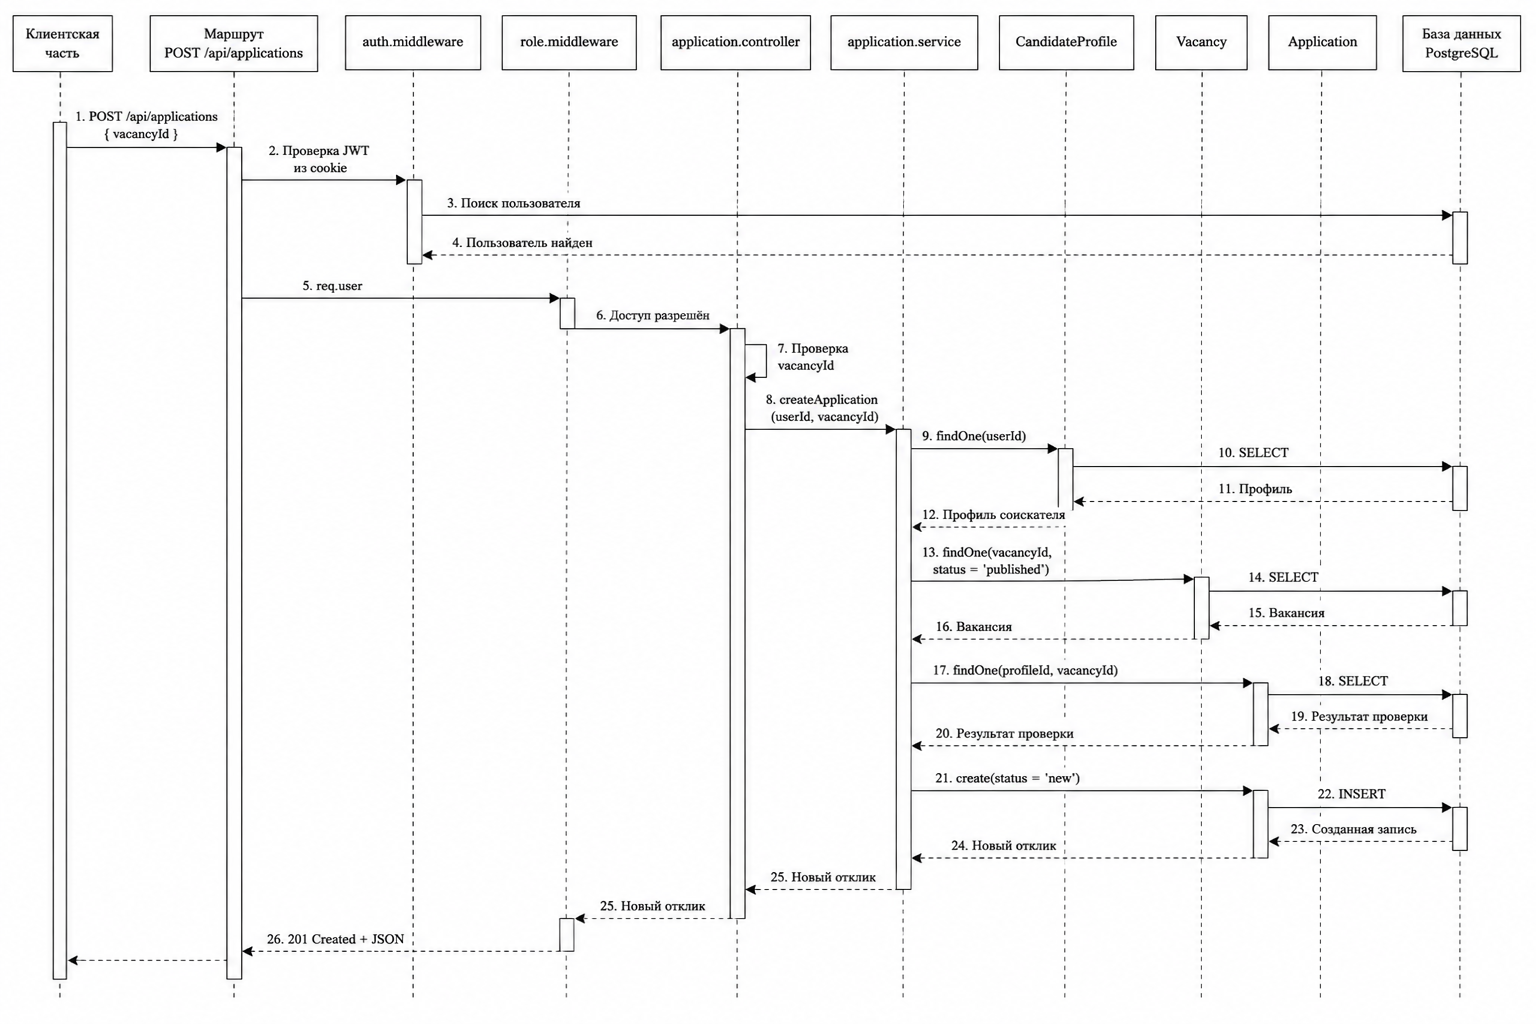
\includegraphics[width=\linewidth]{fig_3_4_request_sequence.png}
	
	\captionof{figure}{Диаграмма последовательности обработки запроса на создание отклика}
	\label{fig:request_sequence}
\end{landscape}
\endgroup

\subsection{Проект базы данных программно-информационной системы}

\subsubsection{ER-модель данных (включая основные сущности и связи)}

ER-модель данных разработанной платформы отражает логическую структуру предметной области и фиксирует основные сущности системы, их смысловые атрибуты и связи между ними. На концептуальном уровне модель описывает пользователей платформы, профессиональные сведения соискателей, данные работодателей, вакансии, навыки, отклики и избранные вакансии. Такая структура соответствует назначению системы, ориентированной на поиск работы и подбор IT-специалистов.

Центральной сущностью модели является пользователь (User), представляющий учётную запись в системе. Для пользователя хранятся адрес электронной почты, хеш пароля, полное имя, роль и признак блокировки. Роль пользователя задаётся значением атрибута и не выносится в самостоятельную сущность, что позволяет использовать единую модель учётной записи для соискателей, работодателей и администраторов.

Сущность CandidateProfile содержит профессиональные сведения соискателя. Она связана с сущностью User отношением «один к одному» на уровне модели предметной области: одному пользователю может соответствовать не более одного профиля соискателя. Профиль включает специализацию, краткое описание и ссылку на GitHub. Таким образом, профессиональные данные соискателя хранятся в отдельной сущности, связанной с его учётной записью.

Сущность Company представляет работодателя как организацию, публикующую вакансии на платформе. Она также связана с User отношением «один к одному»: одному пользователю может соответствовать не более одной компании. В составе сущности хранятся название компании, её описание и адрес веб-сайта. Такое разделение позволяет разграничить общие данные учётной записи и сведения, относящиеся непосредственно к работодателю.

Сущность Vacancy описывает предложение работы, размещаемое компанией. Каждая вакансия связана с одной компанией, при этом одна компания может размещать множество вакансий. В составе вакансии хранятся название, специализация, описание, требования, сведения о заработной плате, местоположение, тип занятости, формат работы, статус публикации и дата создания. Таким образом, между Company и Vacancy реализуется связь «один ко многим».

Сущность Skill используется как справочник навыков, применяемый в системе для описания требований вакансий и профессиональных характеристик соискателей. Связь между профилем соискателя и навыком реализуется через ассоциативную сущность CandidateSkill, что соответствует отношению «многие ко многим». Аналогично связь между вакансией и навыком реализуется через ассоциативную сущность VacancySkill, которая также отражает отношение «многие ко многим». Такое решение позволяет использовать единый перечень навыков для разных объектов предметной области.

Сущность Application фиксирует факт отклика соискателя на конкретную вакансию. Она связывает профиль соискателя и вакансию: один профиль может иметь множество откликов, и одна вакансия может получать множество откликов. В составе отклика хранятся ссылка на профиль, ссылка на вакансию, статус обработки и дата создания. Тем самым сущность Application отражает процесс взаимодействия между соискателем и работодателем в рамках конкретной вакансии.

Сущность FavoriteVacancy реализует связь между пользователем и вакансиями, добавленными в избранное. В данном случае избранное связано именно с учётной записью пользователя, а не с профилем соискателя. Это позволяет хранить перечень вакансий, отмеченных пользователем для последующего просмотра, в виде отдельной ассоциативной сущности, формирующей отношение «многие ко многим» между User и Vacancy.

В целом ER-модель образует целостную структуру, в которой учётная запись пользователя служит отправной точкой для ролевых сценариев работы с системой, компании размещают вакансии, соискатели ведут профессиональный профиль и откликаются на вакансии, а навыки используются как общий справочник для описания требований и компетенций. ER-диаграмма, отражающая указанные сущности и связи между ними, представлена на рисунке 3.5.

\begin{figure}[H]
	\centering
	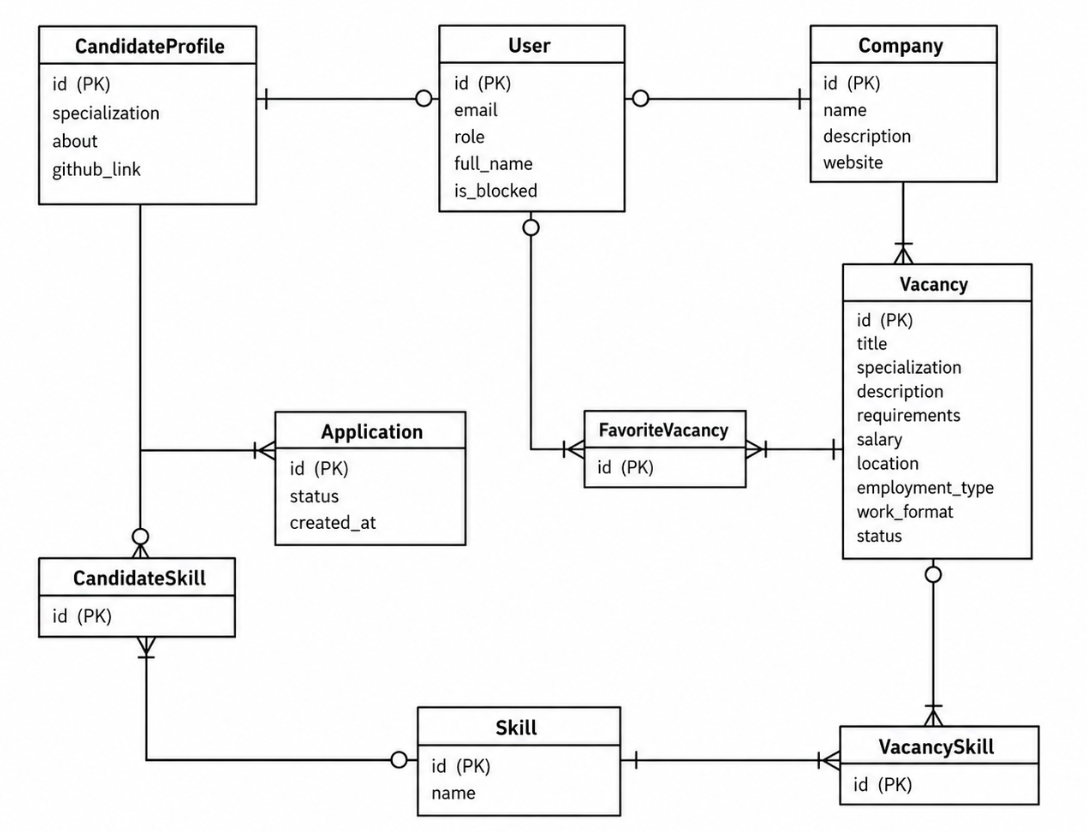
\includegraphics[width=\linewidth]{fig_3_5_er_diagram.png}
	\caption{ER-диаграмма базы данных}
	\label{fig:er_diagram}
\end{figure}

\subsubsection{Нормализация}

Структура базы данных разработанной платформы построена таким образом, чтобы минимизировать дублирование данных и разделить сведения по самостоятельным сущностям в соответствии с их назначением. Выделение отдельных таблиц для пользователей, профилей соискателей, компаний, вакансий, навыков, откликов и избранных вакансий позволяет хранить данные раздельно и связывать их между собой через первичные и внешние ключи. Такое проектное решение соответствует принципам нормализации и обеспечивает логически согласованную организацию данных.

Первая нормальная форма обеспечивается тем, что каждая таблица имеет первичный ключ, а значения атрибутов хранятся в отдельных полях записей. В модели отсутствуют повторяющиеся группы атрибутов внутри одной таблицы: сведения о пользователе хранятся в таблице User, профессиональные данные соискателя — в CandidateProfile, сведения о работодателе — в Company, а информация о вакансии — в Vacancy. Благодаря этому данные предметной области не объединяются в одну крупную запись, а распределяются по специализированным сущностям.

Признаки второй нормальной формы проявляются в том, что данные, относящиеся к разным объектам предметной области, вынесены в отдельные таблицы и не зависят от части составного отношения. Это особенно заметно в таблицах, реализующих связи между сущностями. Например, связь между профилем соискателя и навыком оформлена через таблицу CandidateSkill, а связь между вакансией и навыком — через таблицу VacancySkill. Аналогично добавление вакансии в избранное вынесено в таблицу FavoriteVacancy, а факт отклика на вакансию — в таблицу Application. Благодаря такому разбиению информация о навыках, откликах и избранных вакансиях не дублируется в основных таблицах и хранится в виде самостоятельных связующих сущностей.

Третья нормальная форма обеспечивается тем, что сведения, логически относящиеся к отдельным объектам, не переносятся в зависимые таблицы. Так, данные компании хранятся в таблице Company и связываются с вакансиями через внешний ключ companyId, поэтому сведения о работодателе не дублируются в каждой записи Vacancy. Аналогично сведения о пользователе хранятся в таблице User, тогда как профессиональные характеристики соискателя вынесены в CandidateProfile и связаны с учётной записью через userId. Это устраняет транзитивное дублирование и позволяет изменять данные пользователя, профиля или компании независимо друг от друга.

Дополнительным примером нормализованной структуры является использование таблицы Skill как общего справочника навыков. Вместо хранения текстовых названий навыков непосредственно в профилях соискателей и вакансиях используется единая сущность Skill, связанная с ними через отдельные ассоциативные таблицы. Это позволяет исключить повторение одинаковых значений навыков в разных частях базы данных и упростить поддержку единого перечня компетенций.

Таким образом, структура базы данных платформы соответствует требованиям нормализации на уровне, достаточном для рассматриваемой предметной области. Разделение данных по самостоятельным сущностям, использование внешних ключей и вынесение связей «многие ко многим» в отдельные таблицы позволяют уменьшить избыточность, упростить сопровождение схемы и снизить вероятность аномалий при добавлении, обновлении и удалении данных.

\subsubsection{Реляционная модель данных}

На основе ER-модели, представленной в подразделе 3.5.1, построена реляционная модель базы данных, в которой сущности предметной области представлены в виде таблиц, а связи между ними реализованы посредством первичных и внешних ключей. Реляционная модель определяет состав таблиц, их атрибуты и ограничения целостности, используемые в схеме базы данных платформы. В состав модели входят таблицы users, candidate\_profiles, companies, vacancies, skills, candidate\_skills, vacancy\_skills, applications и favorite\_vacancies.

Для идентификации записей в основных таблицах используются суррогатные первичные ключи id типа BIGINT с автоинкрементом. Такой подход обеспечивает однозначную идентификацию каждой записи и упрощает построение внешних связей между таблицами. Аналогичное решение применяется в таблицах users, vacancies и applications, а также в остальных сущностях схемы базы данных.

Связь между таблицами users и candidate\_profiles реализуется через внешний ключ user\_id, для которого установлено ограничение уникальности. Это означает, что одной учётной записи может соответствовать не более одного профиля соискателя. Аналогичным образом таблица companies связана с users через внешний ключ user\_id с ограничением уникальности, что задаёт отношение «один пользователь — не более одной компании». Таблица vacancies связана с companies через внешний ключ company\_id, благодаря чему одной компании может принадлежать множество вакансий.

Таблица applications связывает вакансии и профили соискателей через внешние ключи vacancy\_id и profile\_id. Для комбинации этих полей установлено ограничение уникальности, исключающее повторную подачу отклика одним и тем же соискателем на одну и ту же вакансию. По аналогичному принципу таблицы candidate\_skills и vacancy\_skills реализуют связи «многие ко многим» между профилями соискателей и навыками, а также между вакансиями и навыками. В таблице favorite\_vacancies связь между пользователем и вакансией также оформлена через пару внешних ключей user\_id и vacancy\_id с ограничением уникальности.

На уровне схемы базы данных определены ограничения целостности, соответствующие логике предметной области. В таблице users поле email имеет ограничение уникальности, исключающее регистрацию нескольких пользователей с одним и тем же адресом электронной почты. Для обязательных атрибутов основных сущностей используются ограничения NOT NULL, например для полей email, password\_hash, role в таблице users, а также для title, specialization, description, requirements, employment\_type, work\_format и status в таблице vacancies.

Допустимые значения ряда атрибутов контролируются не только на уровне приложения, но и на уровне схемы базы данных. В частности, для поля role таблицы users, а также для статусных и классификационных полей таблиц vacancies и applications заданы CHECK-ограничения, фиксирующие допустимые значения ролей, статусов вакансий и откликов, типов занятости и форматов работы. Это повышает надёжность хранения данных и снижает риск записи значений, не соответствующих предметной области системы.

Таким образом, реляционная модель базы данных платформы представляет собой набор взаимосвязанных таблиц, отражающих пользователей, профили соискателей, компании, вакансии, навыки, отклики и избранные вакансии. Использование первичных и внешних ключей, ограничений уникальности, NOT NULL и CHECK обеспечивает целостность данных и соответствует требованиям, предъявляемым к хранению информации в разработанной системе.

\subsubsection{Описание структуры таблиц}

Реляционная модель базы данных реализована в виде набора взаимосвязанных таблиц, соответствующих основным сущностям предметной области. В данном подразделе приводится краткое описание назначения таблиц и их роли в логике работы программной системы. Детальная структура каждой таблицы представлена непосредственно в соответствующей таблице.

Таблица \texttt{users} используется как базовая таблица учётных записей программной системы. Она обеспечивает хранение данных пользователей и служит основой для разграничения доступа между соискателем, работодателем и администратором. Структура таблицы \texttt{users} приведена в таблице~\ref{tab:users}.

\begingroup
\renewcommand{\baselinestretch}{1}\selectfont
\renewcommand{\arraystretch}{1.2}
\setlength{\extrarowheight}{3pt}

\begin{xltabular}{\textwidth}{|C{2.3cm}|C{2.8cm}|>{\raggedright\arraybackslash}m{4.8cm}|C{2.8cm}|C{1.4cm}|}
	\caption{Атрибуты таблицы \texttt{users} (Пользователи)}\label{tab:users}\\ \hline
	Key Type & Optionality & \multicolumn{1}{c|}{Column name} & Data Type & Size \\ \hline
	PK & * & id & BIGINT & \\ \hline
	UK & * & email & VARCHAR & 255 \\ \hline
	& * & password\_hash & VARCHAR & 255 \\ \hline
	& * & role & VARCHAR & 20 \\ \hline
	& * & full\_name & VARCHAR & 255 \\ \hline
	&   & is\_blocked & BOOLEAN & \\ \hline
\end{xltabular}

\endgroup

Таблица \texttt{candidate\_profiles} предназначена для хранения профессионального профиля соискателя. В рамках разработанной системы этот профиль выполняет роль резюме, поэтому отдельная сущность резюме не создаётся. Таблица используется при просмотре и фильтрации кандидатов работодателем. Структура таблицы \texttt{candidate\_profiles} приведена в таблице~\ref{tab:candidate_profiles}.

\begingroup
\renewcommand{\baselinestretch}{1}\selectfont
\renewcommand{\arraystretch}{1.2}
\setlength{\extrarowheight}{3pt}

\begin{xltabular}{\textwidth}{|C{2.3cm}|C{2.8cm}|>{\raggedright\arraybackslash}m{4.8cm}|C{2.8cm}|C{1.4cm}|}
	\caption{Атрибуты таблицы \texttt{candidate\_profiles} (Профили соискателей)}\label{tab:candidate_profiles}\\ \hline
	Key Type & Optionality & \multicolumn{1}{c|}{Column name} & Data Type & Size \\ \hline
	PK & * & id & BIGINT & \\ \hline
	FK, UK & * & user\_id & BIGINT & \\ \hline
	& * & specialization & VARCHAR & 100 \\ \hline
	&   & about & TEXT & \\ \hline
	&   & github\_link & VARCHAR & 255 \\ \hline
\end{xltabular}

\endgroup

Таблица \texttt{companies} используется для хранения сведений об организациях-работодателях. Она связывает работодателя с компанией, от имени которой создаются и публикуются вакансии. Структура таблицы \texttt{companies} приведена в таблице~\ref{tab:companies}.

\begingroup
\renewcommand{\baselinestretch}{1}\selectfont
\renewcommand{\arraystretch}{1.2}
\setlength{\extrarowheight}{3pt}

\begin{xltabular}{\textwidth}{|C{2.3cm}|C{2.8cm}|>{\raggedright\arraybackslash}m{4.8cm}|C{2.8cm}|C{1.4cm}|}
	\caption{Атрибуты таблицы \texttt{companies} (Компании)}\label{tab:companies}\\ \hline
	Key Type & Optionality & \multicolumn{1}{c|}{Column name} & Data Type & Size \\ \hline
	PK & * & id & BIGINT & \\ \hline
	FK, UK & * & user\_id & BIGINT & \\ \hline
	& * & name & VARCHAR & 255 \\ \hline
	&   & description & TEXT & \\ \hline
	&   & website & VARCHAR & 255 \\ \hline
\end{xltabular}

\endgroup

Таблица \texttt{vacancies} предназначена для хранения вакансий, создаваемых работодателями. Она отражает основную сущность, через которую соискатель получает информацию о предложении работы, а работодатель управляет публикацией и дальнейшей обработкой откликов. Структура таблицы \texttt{vacancies} приведена в таблице~\ref{tab:vacancies}.

\begingroup
\renewcommand{\baselinestretch}{1}\selectfont
\renewcommand{\arraystretch}{1.2}
\setlength{\extrarowheight}{3pt}

\begin{xltabular}{\textwidth}{|C{2.3cm}|C{2.8cm}|>{\raggedright\arraybackslash}m{4.8cm}|C{2.8cm}|C{1.4cm}|}
	\caption{Атрибуты таблицы \texttt{vacancies} (Вакансии)}\label{tab:vacancies}\\ \hline
	Key Type & Optionality & \multicolumn{1}{c|}{Column name} & Data Type & Size \\ \hline
	PK & * & id & BIGINT & \\ \hline
	FK & * & company\_id & BIGINT & \\ \hline
	& * & title & VARCHAR & 255 \\ \hline
	& * & specialization & VARCHAR & 100 \\ \hline
	& * & description & TEXT & \\ \hline
	& * & requirements & TEXT & \\ \hline
	&   & salary & VARCHAR & 100 \\ \hline
	&   & location & VARCHAR & 255 \\ \hline
	& * & employment\_type & VARCHAR & \\ \hline
	& * & work\_format & VARCHAR & \\ \hline
	& * & status & VARCHAR & \\ \hline
	&   & created\_at & DATE & \\ \hline
\end{xltabular}

\endgroup

Таблица \texttt{skills} представляет единый справочник навыков, используемых в системе. Наличие отдельного справочника позволяет применять один и тот же перечень компетенций как для описания профилей соискателей, так и для указания требований вакансий. Структура таблицы \texttt{skills} приведена в таблице~\ref{tab:skills}.

\newpage
\begingroup
\renewcommand{\baselinestretch}{1}\selectfont
\renewcommand{\arraystretch}{1.2}
\setlength{\extrarowheight}{3pt}

\begin{xltabular}{\textwidth}{|C{2.3cm}|C{2.8cm}|>{\raggedright\arraybackslash}m{4.8cm}|C{2.8cm}|C{1.4cm}|}
	\caption{Атрибуты таблицы \texttt{skills} (Навыки)}\label{tab:skills}\\ \hline
	Key Type & Optionality & \multicolumn{1}{c|}{Column name} & Data Type & Size \\ \hline
	PK & * & id & BIGINT & \\ \hline
	UK & * & name & VARCHAR & 100 \\ \hline
\end{xltabular}

\endgroup

Таблица \texttt{candidate\_skills} используется для связи профилей соискателей с навыками. Она позволяет одному профилю иметь несколько навыков и одновременно использовать один и тот же навык в разных профилях. Структура таблицы \texttt{candidate\_skills} приведена в таблице~\ref{tab:candidate_skills}.

\begingroup
\renewcommand{\baselinestretch}{1}\selectfont
\renewcommand{\arraystretch}{1.2}
\setlength{\extrarowheight}{3pt}

\begin{xltabular}{\textwidth}{|C{2.3cm}|C{2.8cm}|>{\raggedright\arraybackslash}m{4.8cm}|C{2.8cm}|C{1.4cm}|}
	\caption{Атрибуты таблицы \texttt{candidate\_skills} (Навыки соискателей)}\label{tab:candidate_skills}\\ \hline
	Key Type & Optionality & \multicolumn{1}{c|}{Column name} & Data Type & Size \\ \hline
	PK & * & id & BIGINT & \\ \hline
	FK & * & profile\_id & BIGINT & \\ \hline
	FK & * & skill\_id & BIGINT & \\ \hline
\end{xltabular}

\endgroup

Таблица \texttt{vacancy\_skills} используется для связи вакансий с навыками. Она позволяет работодателю указывать несколько требуемых компетенций для одной вакансии и переиспользовать общий справочник навыков в разных вакансиях. Структура таблицы \texttt{vacancy\_skills} приведена в таблице~\ref{tab:vacancy_skills}.

\begingroup
\renewcommand{\baselinestretch}{1}\selectfont
\renewcommand{\arraystretch}{1.2}
\setlength{\extrarowheight}{3pt}

\begin{xltabular}{\textwidth}{|C{2.3cm}|C{2.8cm}|>{\raggedright\arraybackslash}m{4.8cm}|C{2.8cm}|C{1.4cm}|}
	\caption{Атрибуты таблицы \texttt{vacancy\_skills} (Навыки вакансий)}\label{tab:vacancy_skills}\\ \hline
	Key Type & Optionality & \multicolumn{1}{c|}{Column name} & Data Type & Size \\ \hline
	PK & * & id & BIGINT & \\ \hline
	FK & * & vacancy\_id & BIGINT & \\ \hline
	FK & * & skill\_id & BIGINT & \\ \hline
\end{xltabular}

\endgroup

Таблица \texttt{applications} фиксирует факт отклика соискателя на конкретную вакансию. Она используется для организации процесса рассмотрения кандидата работодателем и отслеживания состояния отклика в рамках пользовательского сценария подбора. Структура таблицы \texttt{applications} приведена в таблице~\ref{tab:applications}.

\begingroup
\renewcommand{\baselinestretch}{1}\selectfont
\renewcommand{\arraystretch}{1.2}
\setlength{\extrarowheight}{3pt}

\begin{xltabular}{\textwidth}{|C{2.3cm}|C{2.8cm}|>{\raggedright\arraybackslash}m{4.8cm}|C{2.8cm}|C{1.4cm}|}
	\caption{Атрибуты таблицы \texttt{applications} (Отклики)}\label{tab:applications}\\ \hline
	Key Type & Optionality & \multicolumn{1}{c|}{Column name} & Data Type & Size \\ \hline
	PK & * & id & BIGINT & \\ \hline
	FK & * & vacancy\_id & BIGINT & \\ \hline
	FK & * & profile\_id & BIGINT & \\ \hline
	& * & status & VARCHAR & 20 \\ \hline
	&   & created\_at & DATE & \\ \hline
\end{xltabular}

\endgroup

Таблица \texttt{favorite\_vacancies} предназначена для хранения вакансий, добавленных пользователями в избранное. Она поддерживает сценарий сохранения интересующих предложений для последующего просмотра без дублирования данных о самих вакансиях. Структура таблицы \texttt{favorite\_vacancies} приведена в таблице~\ref{tab:favorite_vacancies}.

\begingroup
\renewcommand{\baselinestretch}{1}\selectfont
\renewcommand{\arraystretch}{1.2}
\setlength{\extrarowheight}{3pt}

\begin{xltabular}{\textwidth}{|C{2.3cm}|C{2.8cm}|>{\raggedright\arraybackslash}m{4.8cm}|C{2.8cm}|C{1.4cm}|}
	\caption{Атрибуты таблицы \texttt{favorite\_vacancies} (Избранные вакансии)}\label{tab:favorite_vacancies}\\ \hline
	Key Type & Optionality & \multicolumn{1}{c|}{Column name} & Data Type & Size \\ \hline
	PK & * & id & BIGINT & \\ \hline
	FK & * & user\_id & BIGINT & \\ \hline
	FK & * & vacancy\_id & BIGINT & \\ \hline
\end{xltabular}

\endgroup

Таким образом, описание структуры таблиц базы данных отражает назначение основных сущностей программной системы и их участие в пользовательских сценариях: регистрации, ведении профилей, публикации вакансий, работе с навыками, отправке откликов и сохранении избранных вакансий. Подробные сведения о составе таблиц приведены непосредственно в таблицах 3.1--3.9.

\subsection{Эксплуатация и развёртывание}

Для развёртывания платформы и обеспечения единообразия программного окружения используется контейнеризация на основе Docker. Такой подход позволяет изолировать основные компоненты системы, упростить запуск приложения и базы данных, а также снизить влияние различий в конфигурации хост-машины при разработке, тестировании и демонстрации проекта. Конфигурация окружения задана в файле docker-compose.yml и предусматривает запуск двух основных сервисов: приложения и базы данных.

Сервис app представляет собой контейнер серверного приложения. Его сборка выполняется на основе локального Dockerfile, в котором в качестве базового образа используется node:22-alpine. В процессе сборки рабочая директория устанавливается в каталог /app, затем копируются файлы зависимостей, выполняется установка пакетов командой npm ci, после чего в контейнер переносится исходный код проекта. В качестве команды запуска используется npm start, а приложение экспонируется на порту 3000.

Сервис db представляет собой контейнер базы данных и использует официальный образ postgres:16-alpine. Для инициализации экземпляра PostgreSQL в конфигурации заданы переменные окружения POSTGRES\_USER, POSTGRES\_PASSWORD и POSTGRES\_DB. Данные базы сохраняются во внешнем томе postgres\_data, что позволяет сохранять состояние БД при перезапуске контейнеров. Для контроля готовности сервиса базы данных используется healthcheck, выполняющий проверку доступности PostgreSQL командой pg\_isready.

Контейнер приложения получает параметры подключения к базе данных через переменные окружения DB\_HOST, DB\_PORT, DB\_USER, DB\_PASSWORD, DB\_NAME и DB\_DIALECT. Внутри конфигурации в качестве хоста базы данных используется имя сервиса db, что обеспечивает взаимодействие между контейнерами в пределах сети Docker Compose. Для запуска приложения только после готовности базы данных в конфигурации сервиса app используется директива depends\_on с условием service\_healthy.

Инициализация схемы базы данных в проекте выполняется не через автоматическое создание таблиц по моделям, а с помощью миграций Sequelize CLI. В составе проекта предусмотрены команды npm run db:migrate, npm run db:seed и npm run db:reset, позволяющие развернуть схему, заполнить справочные данные и при необходимости полностью пересоздать структуру базы данных. Такой подход обеспечивает воспроизводимое создание схемы и согласованность структуры БД с кодом проекта.

Таким образом, выбранный способ развёртывания обеспечивает воспроизводимость программного окружения, изоляцию серверного приложения и базы данных, а также упрощает запуск системы в рамках разработки и демонстрации. Использование Docker Compose, отдельных контейнеров app и db, механизма проверки готовности базы данных и миграций Sequelize CLI соответствует архитектуре разработанной платформы и упрощает её сопровождение.


\ifПрактика{}\else{
   \section{Рабочий проект}

\subsection{Спецификация компонентов программной системы}

В данном подразделе приводится описание основных компонентов разработанной программной системы. Рабочий проект отражает не проектные решения базы данных и архитектуры, рассмотренные ранее, а фактический состав программных компонентов, реализующих функции web-платформы для поиска работы и подбора IT-специалистов.

Разработанная система построена как клиент-серверное web-приложение. Серверная часть обеспечивает обработку запросов, выполнение бизнес-логики, аутентификацию пользователей, разграничение прав доступа и взаимодействие с базой данных. Клиентская часть предоставляет пользователям web-интерфейс для работы с вакансиями, профилями, компаниями, откликами, избранными вакансиями и административными функциями.

Компоненты программной системы сгруппированы по функциональным областям: аутентификация и авторизация, работа с профилем соискателя, управление компаниями работодателей, обработка вакансий, откликов, избранных вакансий и навыков, а также выполнение административных действий. Отдельно рассматривается клиентская часть, обеспечивающая взаимодействие пользователя с системой через страницы web-интерфейса и запросы к серверному приложению.

Модели данных не выделяются в отдельный подраздел рабочего проекта, так как проект базы данных был подробно рассмотрен в разделе 3.5. В данном разделе модели упоминаются в составе тех компонентов, в которых они используются.

\subsubsection{Компоненты аутентификации и авторизации}

Компоненты аутентификации и авторизации обеспечивают регистрацию пользователей, вход в систему, завершение сеанса, получение сведений о текущем пользователе и разграничение доступа к функциям программной системы. Данная подсистема является базовой для работы остальных компонентов, так как большинство операций платформы зависит от роли пользователя и факта его авторизации.

В системе предусмотрена регистрация пользователей с ролями соискателя и работодателя. При регистрации пользователь указывает адрес электронной почты, пароль, имя и роль. Серверная часть выполняет проверку заполнения обязательных полей, проверяет допустимость выбранной роли, контролирует уникальность адреса электронной почты и сохраняет пароль в базе данных в виде хэша. Такой подход исключает хранение паролей в открытом виде.

Вход в систему выполняется по адресу электронной почты и паролю. После успешной проверки учётных данных сервер формирует JWT-токен, содержащий идентификатор пользователя, адрес электронной почты и роль. Сформированный токен сохраняется в cookie, после чего используется при обращении к защищённым маршрутам приложения.

Проверка авторизованного пользователя выполняется промежуточным обработчиком, который извлекает токен из cookie, проверяет его корректность и загружает сведения о пользователе из базы данных. Если токен отсутствует, недействителен или пользователь заблокирован, выполнение защищённого запроса прекращается с соответствующим сообщением об ошибке. Разграничение доступа по ролям реализовано отдельным middleware, который проверяет, входит ли роль текущего пользователя в список ролей, которым разрешено выполнение конкретного действия.

Основные компоненты подсистемы аутентификации и авторизации представлены в таблице \ref{auth:table}.

\renewcommand{\arraystretch}{0.9}
\begin{xltabular}{\textwidth}{|p{4.2cm}|p{4.1cm}|X|}
	\caption{Компоненты аутентификации и авторизации}
	\label{auth:table}\\
	\hline
	Компонент & Файл & Назначение \\
	\hline
	\endfirsthead
	
	\caption*{Продолжение таблицы \ref{auth:table}}\\
	\hline
	Компонент & Файл & Назначение \\
	\hline
	\finishhead
	
	Маршруты аутентификации & \texttt{auth.routes.js} & Определяют API-маршруты регистрации, входа, получения текущего пользователя и выхода из системы. \\
	\hline
	Контроллер аутентификации & \texttt{auth.controller.js} & Обрабатывает HTTP-запросы, вызывает сервисные функции регистрации и входа, формирует ответ клиентской части, устанавливает и очищает cookie с JWT-токеном. \\
	\hline
	Сервис аутентификации & \texttt{auth.service.js} & Реализует основную логику регистрации и входа: проверку входных данных, проверку уникальности электронной почты, хэширование пароля, проверку пароля и признака блокировки пользователя. \\
	\hline
	Генератор токена & \texttt{generate-token.js} & Формирует JWT-токен на основе идентификатора пользователя, электронной почты и роли пользователя. \\
	\hline
	Middleware авторизации & \texttt{auth.middleware.js} & Проверяет наличие и корректность JWT-токена, получает данные пользователя из базы данных и добавляет их в объект запроса для дальнейшей обработки. \\
	\hline
	Middleware проверки ролей & \texttt{role.middleware.js} & Ограничивает доступ к маршрутам в зависимости от роли пользователя и предотвращает выполнение действий, не предусмотренных для соответствующей роли. \\
	\hline
	Модель пользователя & \texttt{user.js} & Хранит учётные данные пользователя, его роль, ФИО и признак блокировки, а также связывает пользователя с профилем соискателя, компанией и избранными вакансиями. \\
	\hline
\end{xltabular}
\renewcommand{\arraystretch}{1.0}

Таким образом, подсистема аутентификации и авторизации обеспечивает защищённый доступ к функциям web-платформы, связывает пользователя с его ролью и создаёт основу для разграничения возможностей соискателя, работодателя и администратора.


\subsubsection{Компоненты работы с профилем соискателя}

Компоненты работы с профилем соискателя обеспечивают создание, просмотр и редактирование профессиональной информации пользователя с ролью соискателя. Профиль используется для хранения сведений о специализации, описания опыта и ссылки на GitHub-профиль, а также для связи соискателя с набором профессиональных навыков и откликами на вакансии.

Создание профиля доступно только авторизованному пользователю с ролью соискателя. При создании профиля серверная часть проверяет наличие обязательного поля специализации, корректность переданных текстовых данных и отсутствие уже созданного профиля у текущего пользователя. Это ограничение необходимо для того, чтобы одному пользователю соответствовал только один профиль соискателя.

Редактирование профиля также выполняется только владельцем профиля. Перед изменением данных сервер проверяет существование профиля и принадлежность профиля текущему пользователю. Пользователь может изменить специализацию, описание и ссылку на GitHub. Если запрос не содержит данных для изменения, сервер возвращает сообщение об ошибке.

Отдельной частью компонента является управление навыками соискателя. При добавлении навыка выполняется проверка названия навыка, поиск уже существующего навыка в базе данных и создание нового навыка при его отсутствии. Связь между профилем и навыком сохраняется через промежуточную таблицу. Если указанный навык уже добавлен в профиль, повторное добавление не выполняется. Удаление навыка из профиля также доступно только владельцу профиля.

Для работодателя реализован просмотр профилей соискателей. Работодатель может получить список профилей, а также просмотреть конкретный профиль по идентификатору. При получении списка поддерживается фильтрация по специализации и навыку, что позволяет использовать профиль соискателя не только как личную карточку пользователя, но и как источник данных для поиска кандидатов.

Основные компоненты работы с профилем соискателя представлены в таблице \ref{candidateProfile:table}.

\renewcommand{\arraystretch}{0.9}
\begin{xltabular}{\textwidth}{|p{4.0cm}|p{4.9cm}|>{\raggedright\arraybackslash}X|}
	\caption{Компоненты работы с профилем соискателя\label{candidateProfile:table}}\\
	\hline
	Компонент & Файл & Назначение \\
	\hline
	\endfirsthead
	
	\caption*{Продолжение таблицы \ref{candidateProfile:table}}\\
	\hline
	Компонент & Файл & Назначение \\
	\hline
	\endhead
	
	Маршруты профиля соискателя & \texttt{candidate-profile.}\newline\texttt{routes.js} & Определяют API-маршруты создания, получения и редактирования профиля соискателя, управления навыками, а также просмотра профилей соискателей работодателем. \\
	\hline
	Контроллер профиля соискателя & \texttt{candidate-profile.}\newline\texttt{controller.js} & Обрабатывает запросы, связанные с профилем соискателя: создание профиля, получение собственного профиля, обновление данных, добавление и удаление навыков, получение списка профилей и просмотр профиля по идентификатору. \\
	\hline
	Модель профиля соискателя & \texttt{candidateProfile.js} & Хранит сведения о специализации, описании и ссылке на GitHub, связывает профиль с пользователем, навыками и откликами на вакансии. \\
	\hline
	Модель навыка & \texttt{skill.js} & Хранит справочник навыков, которые могут быть связаны с профилями соискателей и вакансиями. \\
	\hline
	Связующая модель навыков соискателя & \texttt{candidateSkill.js} & Реализует связь между профилем соискателя и навыком, позволяя одному профилю иметь несколько навыков. \\
	\hline
	Модель пользователя & \texttt{user.js} & Используется для связи профиля соискателя с учётной записью пользователя и отображения основных сведений о пользователе при просмотре профиля работодателем. \\
	\hline
\end{xltabular}
\renewcommand{\arraystretch}{1.0}

Таким образом, компоненты работы с профилем соискателя обеспечивают хранение профессиональной информации пользователя, управление навыками и предоставляют работодателю возможность поиска кандидатов по специализации и набору навыков.

\subsubsection{Компоненты работы с компаниями работодателей}

Компоненты работы с компаниями работодателей обеспечивают создание, просмотр и редактирование профиля компании, от имени которой работодатель публикует вакансии. Данный компонент связывает учётную запись работодателя с информацией об организации и используется в дальнейшем при создании и отображении вакансий.

Создание компании доступно только авторизованному пользователю с ролью работодателя. При создании профиля компании серверная часть проверяет наличие обязательного поля названия компании, а также корректность переданных текстовых данных. Для одного работодателя допускается создание только одной компании, поэтому перед сохранением новой записи выполняется проверка существования компании, связанной с текущим пользователем.

Получение сведений о компании выполняется двумя способами. Работодатель может получить данные собственной компании, связанные с его учётной записью. Также предусмотрено получение компании по идентификатору, что используется при просмотре сведений о работодателе и связанных с ним вакансиях. При обращении к несуществующей компании сервер возвращает сообщение об ошибке.

Редактирование компании выполняется только владельцем соответствующего профиля. Перед изменением данных серверная часть получает компанию текущего работодателя и проверяет, совпадает ли её идентификатор с идентификатором, указанным в запросе. Если пользователь пытается изменить чужую компанию, выполнение операции запрещается. Работодатель может изменить название компании, описание и адрес сайта.

Модель компании связана с моделью пользователя и моделью вакансии. Связь с пользователем позволяет определить владельца компании, а связь с вакансиями позволяет отображать список вакансий, опубликованных конкретным работодателем.

Основные компоненты работы с компаниями работодателей представлены в таблице \ref{company:table}.

\renewcommand{\arraystretch}{0.9}
\begin{xltabular}{\textwidth}{|p{4.4cm}|p{4.2cm}|X|}
	\caption{Компоненты работы с компаниями работодателей\label{company:table}}\\
	\hline
	Компонент & Файл & Назначение \\
	\hline
	\endfirsthead
	
	\caption*{Продолжение таблицы \ref{company:table}}\\
	\hline
	Компонент & Файл & Назначение \\
	\hline
	\endhead
	
	Маршруты компаний & \texttt{company.routes.js} & Определяют API-маршруты получения собственной компании, создания компании, редактирования компании и получения компании по идентификатору. \\
	\hline
	Контроллер компаний & \texttt{company.controller.js} & Обрабатывает запросы, связанные с компаниями работодателей: получение компании текущего пользователя, создание нового профиля компании, обновление данных компании и получение компании по идентификатору. \\
	\hline
	Модель компании & \texttt{company.js} & Хранит название компании, описание и адрес сайта, связывает компанию с учётной записью работодателя и опубликованными вакансиями. \\
	\hline
	Модель пользователя & \texttt{user.js} & Используется для определения работодателя, которому принадлежит компания. \\
	\hline
	Модель вакансии & \texttt{vacancy.js} & Используется для связи компании с вакансиями, которые публикуются работодателем от имени данной компании. \\
	\hline
	Middleware авторизации & \texttt{auth.middleware.js} & Проверяет, что пользователь авторизован перед выполнением операций с компанией. \\
	\hline
	Middleware проверки ролей & \texttt{role.middleware.js} & Ограничивает доступ к операциям с компаниями только для пользователей с ролью работодателя. \\
	\hline
\end{xltabular}
\renewcommand{\arraystretch}{1.0}

Таким образом, компоненты работы с компаниями работодателей обеспечивают хранение сведений об организации, связывают работодателя с публикуемыми вакансиями и предотвращают изменение данных компании пользователями, не являющимися её владельцами.

\subsubsection{Компоненты работы с вакансиями}

Компоненты работы с вакансиями обеспечивают создание, просмотр, редактирование, публикацию и снятие с публикации предложений о работе. Вакансия является одной из центральных сущностей программной системы, так как через неё осуществляется взаимодействие между работодателем и соискателем.

Создание вакансии доступно авторизованному пользователю с ролью работодателя. Перед созданием вакансии серверная часть проверяет наличие у работодателя профиля компании, так как каждая вакансия должна быть связана с конкретной организацией. При обработке запроса проверяется заполнение обязательных полей: названия вакансии, специализации, описания, требований, типа занятости и формата работы. Также выполняется проверка допустимости значений перечислимых полей, таких как тип занятости и формат работы.

После создания вакансия сохраняется со статусом черновика. Такой подход позволяет работодателю сначала подготовить описание вакансии, а затем отдельно опубликовать её. Опубликованные вакансии доступны для просмотра всем пользователям, включая неавторизованных посетителей. При получении списка опубликованных вакансий поддерживается поиск и фильтрация по ключевым параметрам, включая поисковую строку, специализацию, формат работы, тип занятости и навык.

Редактирование вакансии доступно только работодателю, которому принадлежит компания, разместившая данную вакансию. Перед изменением данных серверная часть проверяет существование компании текущего пользователя, наличие указанной вакансии и её принадлежность данной компании. Если пользователь пытается изменить чужую вакансию, операция не выполняется. При редактировании допускается изменение текстовых данных, сведений о зарплате и местоположении, а также типа занятости и формата работы.

Публикация вакансии переводит её в статус опубликованной, после чего она становится доступной в общем списке вакансий. Снятие с публикации переводит вакансию в архивный статус. Для работодателя такая операция используется для управления собственными вакансиями, а для администратора — в рамках модерации содержимого платформы.

Отдельной частью компонента является управление навыками вакансии. Работодатель может добавить к вакансии требуемый навык или удалить ранее добавленный навык. При добавлении навыка сервер проверяет наличие названия навыка, ищет существующую запись в справочнике навыков и создаёт новую запись при её отсутствии. Повторное добавление одного и того же навыка к вакансии не допускается.

Основные компоненты работы с вакансиями представлены в таблице \ref{vacancy:table}.

\renewcommand{\arraystretch}{0.9}
\begin{xltabular}{\textwidth}{|p{4.4cm}|p{4.2cm}|X|}
	\caption{Компоненты работы с вакансиями\label{vacancy:table}}\\
	\hline
	Компонент & Файл & Назначение \\
	\hline
	\endfirsthead
	
	\caption*{Продолжение таблицы \ref{vacancy:table}}\\
	\hline
	Компонент & Файл & Назначение \\
	\hline
	\endhead
	
	Маршруты вакансий & \texttt{vacancy.routes.js} & Определяют API-маршруты создания вакансии, получения опубликованных вакансий, просмотра вакансии по идентификатору, получения вакансий текущего работодателя, редактирования, публикации, снятия с публикации и управления навыками вакансии. \\
	\hline
	Контроллер вакансий & \texttt{vacancy.controller.js} & Обрабатывает HTTP-запросы, связанные с вакансиями, вызывает сервисные функции и формирует ответы клиентской части. \\
	\hline
	Сервис вакансий & \texttt{vacancy.service.js} & Реализует основную бизнес-логику работы с вакансиями: проверку компании работодателя, валидацию обязательных полей, фильтрацию опубликованных вакансий, изменение статуса вакансии и управление навыками. \\
	\hline
	Модель вакансии & \texttt{vacancy.js} & Хранит сведения о вакансии, включая название, специализацию, описание, требования, зарплату, местоположение, тип занятости, формат работы, статус публикации и связь с компанией. \\
	\hline
	Модель компании & \texttt{company.js} & Используется для проверки принадлежности вакансии работодателю и связи вакансии с организацией, разместившей предложение о работе. \\
	\hline
	Модель навыка & \texttt{skill.js} & Используется для хранения справочника навыков, которые могут быть добавлены к вакансии как требования к кандидату. \\
	\hline
	Связующая модель навыков вакансии & \texttt{vacancySkill.js} & Реализует связь между вакансией и навыком, позволяя одной вакансии содержать несколько требуемых навыков. \\
	\hline
	Middleware авторизации & \texttt{auth.middleware.js} & Проверяет авторизацию пользователя перед выполнением операций работодателя с вакансиями. \\
	\hline
	Middleware проверки ролей & \texttt{role.middleware.js} & Ограничивает создание, редактирование, публикацию и снятие вакансий с публикации в зависимости от роли пользователя. \\
	\hline
\end{xltabular}
\renewcommand{\arraystretch}{1.0}

Таким образом, компоненты работы с вакансиями обеспечивают полный жизненный цикл вакансии: от создания черновика работодателем до публикации, поиска соискателями, редактирования, архивирования и связывания с требуемыми профессиональными навыками.

\subsubsection{Компоненты работы с откликами}

Компоненты работы с откликами обеспечивают взаимодействие между соискателем и работодателем после публикации вакансии. Отклик используется для фиксации заинтересованности соискателя в конкретной вакансии и позволяет работодателю рассматривать поступившие заявки от кандидатов.

Создание отклика доступно только авторизованному пользователю с ролью соискателя. Перед созданием отклика серверная часть проверяет наличие профиля соискателя, так как отклик должен быть связан не только с учётной записью пользователя, но и с его профессиональным профилем. Также проверяется существование вакансии и её статус. Отклик может быть создан только на опубликованную вакансию.

Для предотвращения дублирования заявок серверная часть проверяет, не был ли уже создан отклик текущего соискателя на выбранную вакансию. Если отклик уже существует, повторное создание не выполняется, а клиентской части возвращается сообщение об ошибке. При успешном создании отклик получает начальный статус \texttt{new}.

Соискатель может просматривать список собственных откликов. При получении списка откликов сервер возвращает данные о вакансиях, на которые пользователь отправлял заявки, а также сведения о компаниях, разместивших эти вакансии. Это позволяет соискателю отслеживать историю своих обращений и текущий статус каждого отклика.

Работодатель может просматривать отклики, поступившие на принадлежащие ему вакансии. Перед выдачей списка откликов серверная часть проверяет наличие компании у текущего работодателя и принадлежность указанной вакансии данной компании. В ответе возвращаются сведения о профиле соискателя, пользователе и навыках кандидата.

Изменение статуса отклика доступно только работодателю, которому принадлежит вакансия. Для отклика предусмотрены статусы \texttt{new}, \texttt{in\_review}, \texttt{accepted} и \texttt{rejected}. При изменении статуса сервер проверяет допустимость нового значения, существование отклика и принадлежность связанной вакансии компании текущего работодателя.

Основные компоненты работы с откликами представлены в таблице \ref{application:table}.

\renewcommand{\arraystretch}{0.9}
\begin{xltabular}{\textwidth}{|p{4.4cm}|p{4.2cm}|X|}
	\caption{Компоненты работы с откликами\label{application:table}}\\
	\hline
	Компонент & Файл & Назначение \\
	\hline
	\endfirsthead
	
	\caption*{Продолжение таблицы \ref{application:table}}\\
	\hline
	Компонент & Файл & Назначение \\
	\hline
	\endhead
	
	Маршруты откликов & \texttt{application.routes.js} & Определяют API-маршруты создания отклика, получения собственных откликов соискателя и изменения статуса отклика работодателем. \\
	\hline
	Маршрут просмотра откликов на вакансию & \texttt{vacancy.routes.js} & Связывает просмотр откликов с конкретной вакансией работодателя и передаёт обработку в контроллер откликов. \\
	\hline
	Контроллер откликов & \texttt{application.controller.js} & Обрабатывает HTTP-запросы, связанные с откликами: создание отклика, получение откликов соискателя, получение откликов на вакансию работодателя и изменение статуса отклика. \\
	\hline
	Сервис откликов & \texttt{application.service.js} & Реализует бизнес-логику работы с откликами: проверку профиля соискателя, проверку опубликованной вакансии, запрет повторного отклика, получение списков откликов и изменение статуса. \\
	\hline
	Модель отклика & \texttt{application.js} & Хранит связь между вакансией и профилем соискателя, статус отклика и дату его создания. \\
	\hline
	Модель профиля соискателя & \texttt{candidateProfile.js} & Используется для связи отклика с профессиональным профилем пользователя и отображения данных кандидата работодателю. \\
	\hline
	Модель вакансии & \texttt{vacancy.js} & Используется для связи отклика с вакансией и проверки принадлежности вакансии компании работодателя. \\
	\hline
	Модель компании & \texttt{company.js} & Используется при проверке прав работодателя на просмотр и изменение откликов по принадлежащим ему вакансиям. \\
	\hline
	Middleware авторизации & \texttt{auth.middleware.js} & Проверяет авторизацию пользователя перед созданием, просмотром и изменением откликов. \\
	\hline
	Middleware проверки ролей & \texttt{role.middleware.js} & Ограничивает создание отклика ролью соискателя, а изменение статуса и просмотр откликов на вакансию ролью работодателя. \\
	\hline
\end{xltabular}
\renewcommand{\arraystretch}{1.0}

Таким образом, компоненты работы с откликами обеспечивают основной сценарий взаимодействия соискателя и работодателя: отправку заявки на опубликованную вакансию, просмотр истории откликов соискателем, рассмотрение кандидатов работодателем и изменение статуса отклика.

\subsubsection{Компоненты работы с избранными вакансиями}

Компоненты работы с избранными вакансиями обеспечивают сохранение интересующих соискателя предложений о работе в отдельном списке. Данный функционал позволяет пользователю с ролью соискателя вернуться к выбранным вакансиям позже и не выполнять повторный поиск среди общего списка опубликованных предложений.

Добавление вакансии в избранное доступно только авторизованному пользователю с ролью соискателя. Перед выполнением операции серверная часть проверяет корректность идентификатора вакансии, существование вакансии и её статус. В избранное может быть добавлена только опубликованная вакансия, доступная для просмотра пользователями платформы.

Для предотвращения дублирования записей серверная часть проверяет, не была ли выбранная вакансия уже добавлена в избранное текущим пользователем. Если связь между пользователем и вакансией уже существует, повторное добавление не выполняется, а клиентской части возвращается сообщение об ошибке.

Получение списка избранных вакансий выполняется по идентификатору текущего пользователя. При формировании ответа сервер возвращает не только записи избранного, но и связанные с ними сведения о вакансиях и компаниях. Это позволяет клиентской части отобразить пользователю полноценный список сохранённых предложений о работе.

Удаление вакансии из избранного также выполняется только текущим соискателем. Перед удалением сервер проверяет наличие соответствующей записи в избранном. Если вакансия не найдена в списке избранного пользователя, операция не выполняется и возвращается сообщение об ошибке.

Основные компоненты работы с избранными вакансиями представлены в таблице \ref{favorite:table}.

\renewcommand{\arraystretch}{0.9}
\begin{xltabular}{\textwidth}{|p{4.4cm}|p{4.2cm}|X|}
	\caption{Компоненты работы с избранными вакансиями\label{favorite:table}}\\
	\hline
	Компонент & Файл & Назначение \\
	\hline
	\endfirsthead
	
	\caption*{Продолжение таблицы \ref{favorite:table}}\\
	\hline
	Компонент & Файл & Назначение \\
	\hline
	\endhead
	
	Маршруты избранных вакансий & \texttt{favorite.routes.js} & Определяют API-маршруты получения списка избранных вакансий, добавления вакансии в избранное и удаления вакансии из избранного. \\
	\hline
	Контроллер избранных вакансий & \texttt{favorite.controller.js} & Обрабатывает HTTP-запросы, связанные с избранными вакансиями, проверяет корректность идентификатора вакансии и вызывает сервисные функции. \\
	\hline
	Сервис избранных вакансий & \texttt{favorite.service.js} & Реализует бизнес-логику работы с избранным: проверку опубликованной вакансии, запрет повторного добавления, получение списка избранных вакансий и удаление записи из избранного. \\
	\hline
	Модель избранной вакансии & \texttt{favoriteVacancy.js} & Хранит связь между пользователем и вакансией, добавленной в избранное. \\
	\hline
	Модель вакансии & \texttt{vacancy.js} & Используется для проверки существования и статуса вакансии, а также для отображения сведений о сохранённой вакансии. \\
	\hline
	Модель компании & \texttt{company.js} & Используется для отображения сведений о компании, разместившей вакансию, при получении списка избранных вакансий. \\
	\hline
	Middleware авторизации & \texttt{auth.middleware.js} & Проверяет авторизацию пользователя перед выполнением операций с избранными вакансиями. \\
	\hline
	Middleware проверки ролей & \texttt{role.middleware.js} & Ограничивает доступ к операциям с избранными вакансиями только для пользователей с ролью соискателя. \\
	\hline
\end{xltabular}
\renewcommand{\arraystretch}{1.0}

Таким образом, компоненты работы с избранными вакансиями позволяют соискателю сохранять интересующие предложения о работе, просматривать их в отдельном списке и удалять из избранного неактуальные вакансии.

\subsubsection{Компоненты работы с навыками}

Компоненты работы с навыками обеспечивают хранение и использование справочника профессиональных навыков в программной системе. Навыки применяются для описания компетенций соискателей и требований работодателей к кандидатам, поэтому данный компонент связан как с профилями соискателей, так и с вакансиями.

В системе используется единый справочник навыков. Каждая запись справочника содержит уникальное название навыка. Такой подход позволяет избежать дублирования одинаковых навыков и использовать одни и те же значения при заполнении профилей соискателей и описании требований к вакансиям.

Получение списка навыков выполняется через отдельный API-маршрут. Данный маршрут доступен авторизованным пользователям. При обращении к нему серверная часть возвращает список навыков, отсортированный по названию. Такой список может использоваться клиентской частью при выборе навыков для профиля соискателя или вакансии.

Связь навыков с профилями соискателей реализуется через промежуточную модель. Благодаря этому один профиль может иметь несколько навыков, а один и тот же навык может быть указан у разных соискателей. Аналогичным образом навыки связываются с вакансиями: одна вакансия может содержать несколько требуемых навыков, а один навык может использоваться в разных вакансиях.

Навыки также используются при поиске и фильтрации данных. Работодатель может отбирать кандидатов по требуемым навыкам, а соискатель может использовать навыки при поиске подходящих вакансий. Таким образом, компонент работы с навыками выполняет не только справочную, но и связующую функцию между основными сущностями системы.

Основные компоненты работы с навыками представлены в таблице \ref{skill:table}.

\renewcommand{\arraystretch}{0.9}
\begin{xltabular}{\textwidth}{|p{4.4cm}|p{4.2cm}|>{\raggedright\arraybackslash}X|}
	\caption{Компоненты работы с навыками\label{skill:table}}\tabularnewline
	\hline
	Компонент & Файл & Назначение \tabularnewline
	\hline
	\endfirsthead
	
	\caption*{Продолжение таблицы \ref{skill:table}}\tabularnewline
	\hline
	Компонент & Файл & Назначение \tabularnewline
	\hline
	\endhead
	
	Маршруты навыков & \texttt{skill.routes.js} & Определяют API-маршрут получения списка навыков, доступный авторизованным пользователям системы. \tabularnewline
	\hline
	Контроллер навыков & \texttt{skill.controller.js} & Обрабатывает HTTP-запрос на получение списка навыков и формирует ответ клиентской части. \tabularnewline
	\hline
	Сервис навыков & \texttt{skill.service.js} & Получает список навыков из базы данных и сортирует их по названию. \tabularnewline
	\hline
	Модель навыка & \texttt{skill.js} & Хранит уникальные названия навыков и связывает навыки с профилями соискателей и вакансиями. \tabularnewline
	\hline
	Связующая модель навыков соискателя & \texttt{candidateSkill.js} & Реализует связь между профилем соискателя и навыком. \tabularnewline
	\hline
	Связующая модель навыков вакансии & \texttt{vacancySkill.js} & Реализует связь между вакансией и требуемым навыком. \tabularnewline
	\hline
	Модель профиля соискателя & \texttt{candidateProfile.js} & Используется при привязке навыков к профессиональному профилю соискателя. \tabularnewline
	\hline
	Модель вакансии & \texttt{vacancy.js} & Используется при привязке навыков к требованиям конкретной вакансии. \tabularnewline
	\hline
	Middleware авторизации & \texttt{auth.middleware.js} & Проверяет авторизацию пользователя перед получением списка навыков. \tabularnewline
	\hline
\end{xltabular}
\renewcommand{\arraystretch}{1.0}


Таким образом, компоненты работы с навыками обеспечивают единое хранение профессиональных компетенций, связывают профили соискателей с требованиями вакансий и используются при поиске и фильтрации данных в системе.

\subsubsection{Административные компоненты программной системы}

Административные компоненты программной системы предназначены для выполнения действий по контролю пользователей и вакансий. Данный функционал доступен только пользователю с ролью администратора и используется для просмотра данных системы, ограничения доступа нарушающих правила пользователей и удаления некорректных или неактуальных вакансий.

Доступ к административным маршрутам защищён механизмами аутентификации и проверки роли пользователя. Перед выполнением административного действия серверная часть проверяет, что пользователь авторизован и обладает ролью администратора. Это предотвращает доступ обычных соискателей и работодателей к функциям управления системой.

Администратор может получить список пользователей, зарегистрированных в системе. При формировании ответа возвращаются основные сведения об учётных записях: идентификатор, адрес электронной почты, ФИО, роль и признак блокировки. Эти данные позволяют администратору контролировать состав пользователей и при необходимости ограничивать доступ отдельных учётных записей.

Блокировка пользователя выполняется по идентификатору. Перед выполнением операции сервер проверяет корректность переданного идентификатора и существование пользователя. Также предусмотрена дополнительная проверка, запрещающая администратору заблокировать собственную учётную запись. После успешного выполнения операции у пользователя устанавливается признак блокировки.

Администратор также может получить список вакансий, размещённых в системе. При получении списка вакансий дополнительно загружаются сведения о компании, которой принадлежит вакансия. Это позволяет администратору просматривать не только само предложение о работе, но и организацию, от имени которой оно было опубликовано.

Удаление вакансии выполняется по идентификатору. Перед удалением серверная часть проверяет корректность параметра маршрута и существование указанной вакансии. Если вакансия найдена, она удаляется из базы данных. Если вакансия отсутствует, клиентской части возвращается сообщение об ошибке.

Основные административные компоненты программной системы представлены в таблице \ref{admin:table}.

\renewcommand{\arraystretch}{0.9}
\begin{xltabular}{\textwidth}{|p{4.4cm}|p{4.2cm}|X|}
	\caption{Административные компоненты программной системы\label{admin:table}}\\
	\hline
	Компонент & Файл & Назначение \\
	\hline
	\endfirsthead
	
	\caption*{Продолжение таблицы \ref{admin:table}}\\
	\hline
	Компонент & Файл & Назначение \\
	\hline
	\endhead
	
	Административные маршруты & \texttt{admin.routes.js} & Определяют API-маршруты получения списка пользователей, получения списка вакансий, блокировки пользователя и удаления вакансии. \\
	\hline
	Административный контроллер & \texttt{admin.controller.js} & Обрабатывает HTTP-запросы администратора, проверяет корректность идентификаторов в параметрах маршрутов и вызывает сервисные функции. \\
	\hline
	Административный сервис & \texttt{admin.service.js} & Реализует бизнес-логику административных действий: получение пользователей, получение вакансий, блокировку пользователя и удаление вакансии. \\
	\hline
	Модель пользователя & \texttt{user.js} & Используется для получения списка пользователей и изменения признака блокировки учётной записи. \\
	\hline
	Модель вакансии & \texttt{vacancy.js} & Используется для получения списка вакансий и удаления вакансии администратором. \\
	\hline
	Модель компании & \texttt{company.js} & Используется для отображения сведений о компании при получении списка вакансий. \\
	\hline
	Middleware авторизации & \texttt{auth.middleware.js} & Проверяет авторизацию пользователя перед обращением к административным маршрутам. \\
	\hline
	Middleware проверки ролей & \texttt{role.middleware.js} & Ограничивает доступ к административным маршрутам только для пользователя с ролью администратора. \\
	\hline
\end{xltabular}
\renewcommand{\arraystretch}{1.0}

Таким образом, административные компоненты обеспечивают базовое управление пользователями и вакансиями, позволяют ограничивать доступ отдельных учётных записей и поддерживать корректность содержимого платформы.

\subsubsection{Клиентская часть программной системы}

Клиентская часть программной системы предназначена для предоставления пользователям web-интерфейса и организации взаимодействия с серверной частью приложения. Она включает HTML-страницы, CSS-стили и JavaScript-файлы, реализующие обработку пользовательских действий, отправку запросов к API и отображение полученных данных.

HTML-страницы интерфейса сгруппированы по ролям пользователей и основным сценариям работы. Для неавторизованных пользователей предусмотрены страницы регистрации, входа, просмотра списка вакансий и просмотра карточки вакансии. Для соискателя реализованы страницы личного кабинета, профиля, навыков, избранных вакансий и собственных откликов. Для работодателя предусмотрены страницы управления компанией, вакансиями, откликами и просмотра кандидатов. Для администратора реализованы страницы управления пользователями и вакансиями.

JavaScript-файлы клиентской части отвечают за получение данных с сервера, отправку форм, обработку ошибок, обновление содержимого страниц и переходы между сценариями. Общий модуль взаимодействия с API используется для выполнения HTTP-запросов к серверной части. Отдельные скрипты реализуют логику регистрации, входа, защиты страниц личных кабинетов, работы с вакансиями, профилями, откликами, избранным и административными действиями.

Для ограничения доступа к страницам личных кабинетов используется проверка авторизации и роли пользователя. При открытии защищённой страницы клиентская часть обращается к серверу для получения сведений о текущем пользователе. Если пользователь не авторизован или его роль не соответствует странице, выполняется перенаправление на подходящую страницу.

Клиентская часть не содержит бизнес-логику, связанную с изменением данных в базе. Она выполняет роль интерфейсного слоя: собирает данные из форм, отправляет их на сервер, получает результат выполнения операции и отображает пользователю сообщение об успешном выполнении действия или ошибке.

Основные компоненты клиентской части представлены в таблице \ref{client:table}.

\renewcommand{\arraystretch}{0.9}
\begin{xltabular}{\textwidth}{|p{4.4cm}|p{4.2cm}|X|}
	\caption{Компоненты клиентской части программной системы\label{client:table}}\\
	\hline
	Компонент & Файл или каталог & Назначение \\
	\hline
	\endfirsthead
	
	\caption*{Продолжение таблицы \ref{client:table}}\\
	\hline
	Компонент & Файл или каталог & Назначение \\
	\hline
	\endhead
	
	HTML-страницы интерфейса & \texttt{public/pages} & Содержат страницы регистрации, входа, просмотра вакансий, личных кабинетов соискателя, работодателя и администратора. \\
	\hline
	CSS-оформление & \texttt{public/css} & Определяет внешний вид страниц, расположение элементов интерфейса, оформление форм, списков, карточек вакансий и административных страниц. \\
	\hline
	Модуль API-запросов & \texttt{api.js} & Выполняет отправку HTTP-запросов к серверной части и используется другими клиентскими скриптами при обращении к REST API. \\
	\hline
	Модуль авторизации & \texttt{auth.js} & Реализует клиентскую логику регистрации, входа, выхода из системы и получения сведений о текущем пользователе. \\
	\hline
	Проверка доступа к личным кабинетам & \texttt{dashboard-guard.js} & Проверяет авторизацию пользователя и соответствие его роли открываемой странице личного кабинета. \\
	\hline
	Скрипты соискателя & \texttt{candidate-*.js} & Обеспечивают работу страниц профиля соискателя, навыков, избранных вакансий и собственных откликов. \\
	\hline
	Скрипты работодателя & \texttt{employer-*.js} & Обеспечивают работу страниц компании, управления вакансиями, просмотра откликов и поиска кандидатов. \\
	\hline
	Скрипты администратора & \texttt{admin-*.js} & Обеспечивают работу административных страниц управления пользователями и вакансиями. \\
	\hline
	Скрипты вакансий & \texttt{vacancies.js}, \texttt{vacancy-detail.js} & Реализуют отображение списка опубликованных вакансий, фильтрацию и просмотр подробной информации о вакансии. \\
	\hline
\end{xltabular}
\renewcommand{\arraystretch}{1.0}

Таким образом, клиентская часть программной системы обеспечивает доступ пользователей к функциям web-платформы через страницы интерфейса, связывает действия пользователя с серверным API и отображает результаты выполнения операций в зависимости от роли пользователя.

\subsection{Системное тестирование программной системы}

Системное тестирование программной системы выполнялось с целью проверки корректности работы основных функций web-платформы для поиска работы и подбора IT-специалистов. Тестирование проводилось по пользовательским сценариям, связанным с регистрацией, аутентификацией, работой соискателя, работодателя и администратора.

В ходе тестирования проверялись основные функции программной системы: регистрация и вход пользователя, создание и редактирование профиля соискателя, поиск и фильтрация вакансий, отправка отклика, добавление вакансии в избранное, создание компании работодателя, создание и публикация вакансии, просмотр откликов работодателем, изменение статуса отклика, поиск кандидатов, административное управление пользователями и вакансиями, а также разграничение прав доступа.

Тестирование выполнялось вручную через пользовательский web-интерфейс при локальном запуске программной системы. Проверка проводилась в браузере Google Chrome. Серверная часть приложения была запущена на платформе Node.js с использованием фреймворка Express, взаимодействие с базой данных осуществлялось через PostgreSQL и Sequelize ORM. В ходе проверки использовались страницы клиентской части, API-маршруты серверного приложения и данные, сохраняемые в базе данных.

Для каждого тестового сценария были определены предусловия, последовательность действий, ожидаемый результат и фактический результат.


\subsubsection{Сводная таблица тест-кейсов}

Сводный перечень тест-кейсов, использованных при системном тестировании программной системы, представлен в таблице \ref{testCases:table}.

\renewcommand{\arraystretch}{0.9}
\begin{xltabular}{\textwidth}{|p{2.2cm}|X|p{3cm}|}
	\caption{Сводная таблица тест-кейсов\label{testCases:table}}\\
	\hline
	ID & Название тест-кейса & Результат \\
	\hline
	\endfirsthead
	
	\caption*{Продолжение таблицы \ref{testCases:table}}\\
	\hline
	ID & Название тест-кейса & Результат \\
	\hline
	\endhead
	
	TC-01 & Регистрация пользователя & Пройден \\
	\hline
	TC-02 & Вход пользователя в систему & Пройден \\
	\hline
	TC-03 & Создание и редактирование профиля соискателя & Пройден \\
	\hline
	TC-04 & Поиск и фильтрация вакансий & Пройден \\
	\hline
	TC-05 & Отклик на вакансию & Пройден \\
	\hline
	TC-06 & Добавление вакансии в избранное & Пройден \\
	\hline
	TC-07 & Создание и редактирование компании & Пройден \\
	\hline
	TC-08 & Создание и публикация вакансии & Пройден \\
	\hline
	TC-09 & Просмотр откликов работодателем & Пройден \\
	\hline
	TC-10 & Изменение статуса отклика & Пройден \\
	\hline
	TC-11 & Поиск и фильтрация кандидатов & Пройден \\
	\hline
	TC-12 & Административное управление пользователями и вакансиями & Пройден \\
	\hline
	TC-13 & Проверка разграничения прав доступа & Пройден \\
	\hline
\end{xltabular}
\renewcommand{\arraystretch}{1.0}

\subsubsection{TC-01. Регистрация пользователя}

Цель тест-кейса: проверить корректность регистрации нового пользователя в системе.

Предусловие: пользователь находится на странице регистрации, в системе отсутствует учётная запись с указанным адресом электронной почты.

Шаги выполнения тест-кейса:
\begin{enumerate}
	\item Открыть страницу регистрации.
	\item Заполнить поля формы регистрации: ФИО, адрес электронной почты, пароль и роль пользователя.
	\item Выбрать роль соискателя или работодателя.
	\item Нажать кнопку регистрации.
\end{enumerate}

Ожидаемый результат: система проверяет корректность введённых данных, создаёт новую учётную запись пользователя и сообщает об успешной регистрации.

Фактический результат: после отправки формы регистрации новая учётная запись была создана, пользовательские данные сохранились в системе, повторная регистрация с тем же адресом электронной почты не выполняется. Тест-кейс пройден.

На рисунке \ref{tc01:image} представлен результат регистрации пользователя в системе.

\begin{figure}[H]
	\center{
\includegraphics[width=1\linewidth]{tc01_registration.png}}
	\caption{Результат регистрации пользователя}
	\label{tc01:image}
\end{figure}

\subsubsection{TC-02. Вход пользователя в систему}

Цель тест-кейса: проверить корректность входа зарегистрированного пользователя в систему.

Предусловие: в системе существует зарегистрированная учётная запись пользователя, пользователь находится на странице входа.

Шаги выполнения тест-кейса:
\begin{enumerate}
	\item Открыть страницу входа.
	\item Ввести адрес электронной почты зарегистрированного пользователя.
	\item Ввести пароль пользователя.
	\item Нажать кнопку входа.
\end{enumerate}

Ожидаемый результат: система проверяет введённые учётные данные, выполняет вход пользователя и открывает доступ к функциям, соответствующим его роли.

Фактический результат: после ввода корректных учётных данных пользователь успешно входит в систему, сервер создаёт сеанс авторизации, а интерфейс открывает доступ к разделам, соответствующим роли пользователя. Тест-кейс пройден.

На рисунке \ref{tc02:image} представлен личный кабинет соискателя после успешного входа в систему.

\begin{figure}[H]
	\center{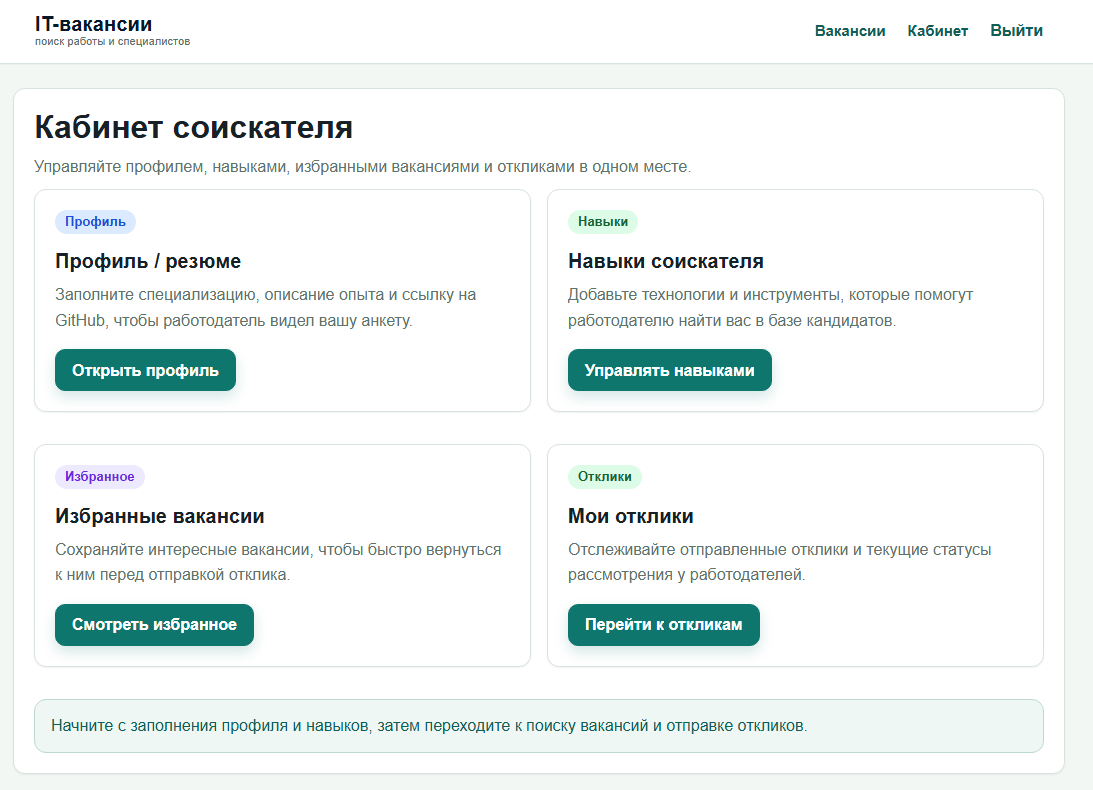
\includegraphics[width=1\linewidth]{tc02_login.png}}
	\caption{Личный кабинет соискателя после входа в систему}
	\label{tc02:image}
\end{figure}

\subsubsection{TC-03. Создание и редактирование профиля соискателя}

Цель тест-кейса: проверить возможность создания и редактирования профиля соискателя.

Предусловие: пользователь зарегистрирован в системе с ролью соискателя и выполнил вход в систему.

Шаги выполнения тест-кейса:
\begin{enumerate}
	\item Открыть личный кабинет соискателя.
	\item Перейти на страницу профиля.
	\item Заполнить сведения о специализации, описании опыта и ссылке на GitHub.
	\item Сохранить профиль.
	\item Изменить одно или несколько полей профиля.
	\item Повторно сохранить изменения.
\end{enumerate}

Ожидаемый результат: система создаёт профиль соискателя, сохраняет введённые данные и позволяет владельцу профиля редактировать их.

Фактический результат: профиль соискателя был создан, сведения о специализации, описании опыта и ссылке на GitHub сохранились в системе. После редактирования обновлённые данные отобразились на странице профиля. Тест-кейс пройден.

На рисунке \ref{tc03:image} представлен результат заполнения профиля соискателя.

\begin{figure}[H]
	\center{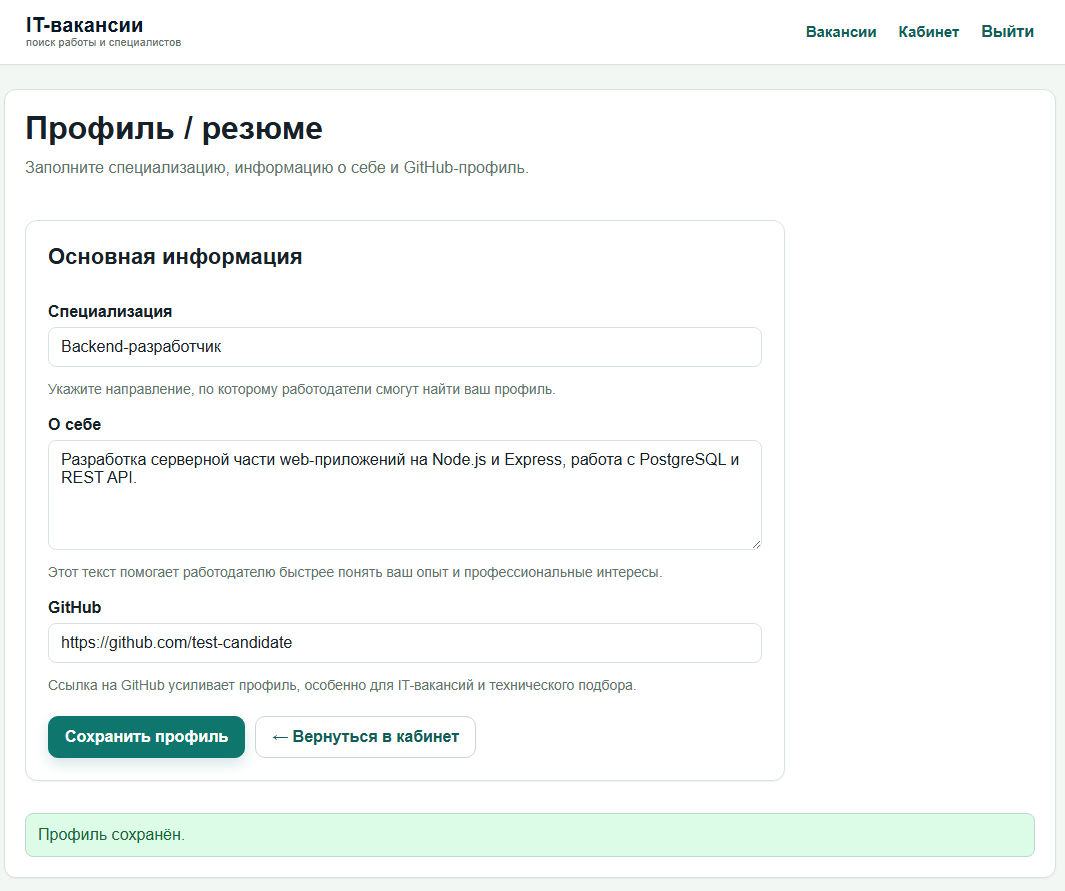
\includegraphics[width=1\linewidth]{tc03_candidate_profile.png}}
	\caption{Заполненный профиль соискателя}
	\label{tc03:image}
\end{figure}

\subsubsection{TC-04. Поиск и фильтрация вакансий}

Цель тест-кейса: проверить корректность поиска и фильтрации опубликованных вакансий.

Предусловие: в системе существуют опубликованные вакансии, пользователь находится на странице списка вакансий.

Шаги выполнения тест-кейса:
\begin{enumerate}
	\item Открыть страницу со списком вакансий.
	\item Ввести поисковый запрос в поле поиска.
	\item Указать параметры фильтрации, например специализацию, формат работы или тип занятости.
	\item Применить фильтр.
	\item Открыть одну из найденных вакансий.
\end{enumerate}

Ожидаемый результат: система отображает список вакансий, соответствующих заданным параметрам поиска и фильтрации, а также позволяет открыть карточку выбранной вакансии.

Фактический результат: после применения параметров поиска и фильтрации список вакансий обновился, в нём остались предложения, соответствующие заданным условиям. Карточка выбранной вакансии открылась и отобразила подробные сведения о вакансии. Тест-кейс пройден.

На рисунке \ref{tc04:image} представлен результат поиска и фильтрации вакансий.

\begin{figure}[H]
	\center{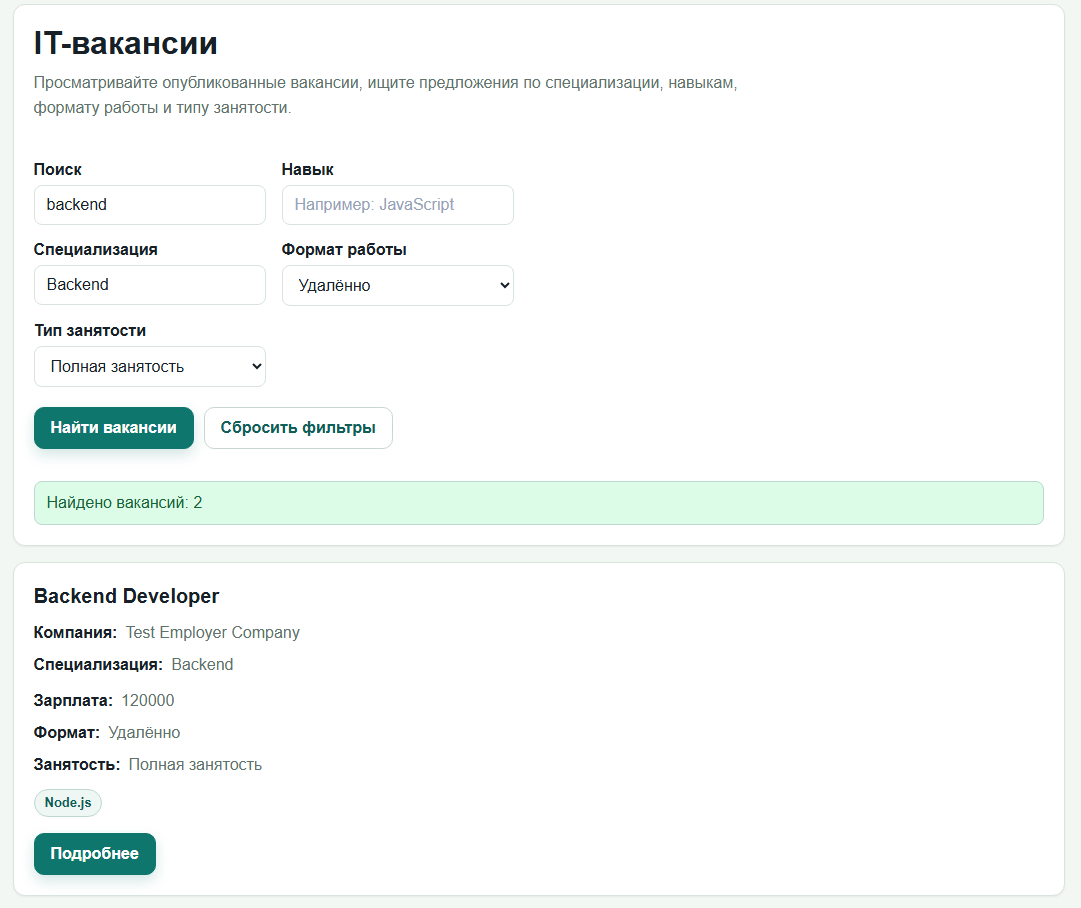
\includegraphics[width=1\linewidth]{tc04_vacancy_filter.png}}
	\caption{Результат поиска и фильтрации вакансий}
	\label{tc04:image}
\end{figure}

\subsubsection{TC-05. Отклик на вакансию}

Цель тест-кейса: проверить возможность отправки отклика соискателем на опубликованную вакансию.

Предусловие: пользователь зарегистрирован с ролью соискателя, выполнил вход в систему, имеет созданный профиль соискателя, в системе существует опубликованная вакансия.

Шаги выполнения тест-кейса:
\begin{enumerate}
	\item Открыть страницу со списком опубликованных вакансий.
	\item Выбрать подходящую вакансию.
	\item Открыть карточку выбранной вакансии.
	\item Нажать кнопку отправки отклика.
	\item Проверить появление отклика в списке собственных откликов соискателя.
\end{enumerate}

Ожидаемый результат: система создаёт отклик на выбранную вакансию, связывает его с профилем соискателя и отображает отклик в списке заявок пользователя.

Фактический результат: после нажатия кнопки отправки отклика в системе была создана запись отклика, связанная с выбранной вакансией и профилем текущего соискателя. Отклик отобразился в списке собственных откликов пользователя и получил начальный статус \texttt{new}. Тест-кейс пройден.

На рисунке \ref{tc05:image} представлен результат отправки отклика на вакансию.

\begin{figure}[H]
	\center{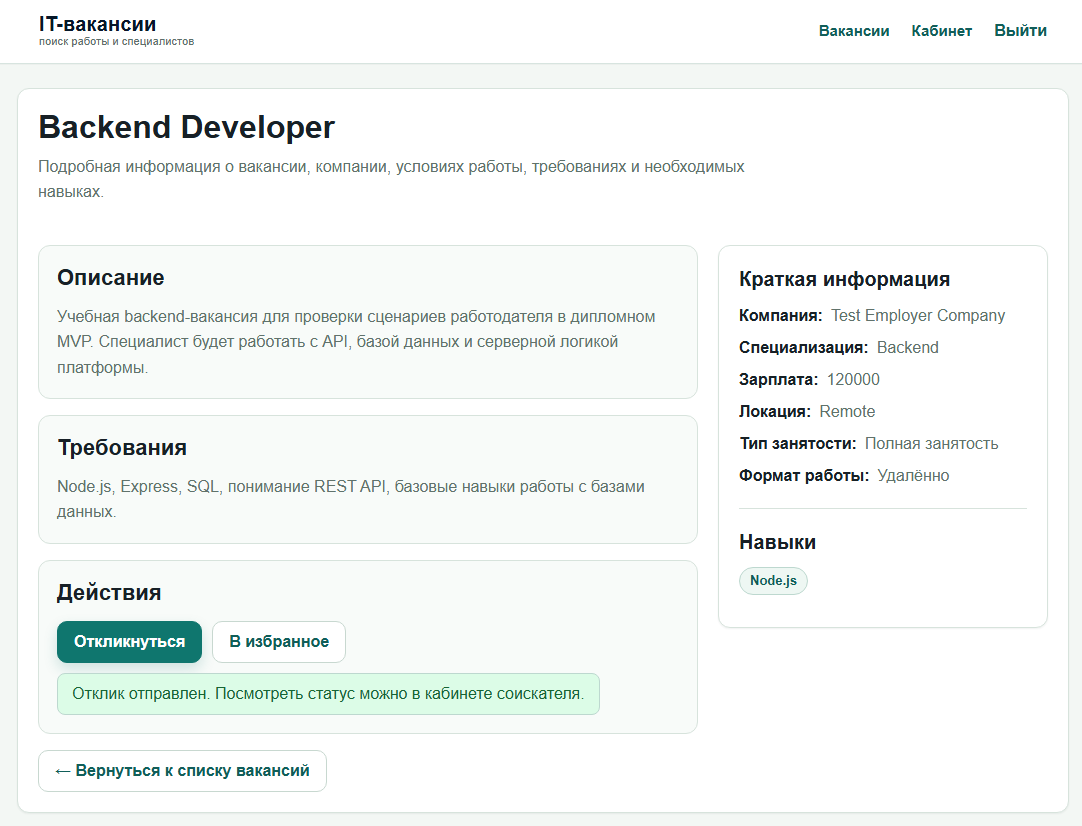
\includegraphics[width=1\linewidth]{tc05_application.png}}
	\caption{Результат отправки отклика на вакансию}
	\label{tc05:image}
\end{figure}

\subsubsection{TC-06. Добавление вакансии в избранное}

Цель тест-кейса: проверить возможность добавления опубликованной вакансии в список избранных вакансий соискателя.

Предусловие: пользователь зарегистрирован с ролью соискателя, выполнил вход в систему, в системе существует опубликованная вакансия.

Шаги выполнения тест-кейса:
\begin{enumerate}
	\item Открыть страницу со списком опубликованных вакансий.
	\item Выбрать интересующую вакансию.
	\item Нажать кнопку добавления вакансии в избранное.
	\item Перейти в раздел избранных вакансий.
	\item Проверить наличие выбранной вакансии в списке избранного.
\end{enumerate}

Ожидаемый результат: система добавляет выбранную вакансию в список избранных вакансий текущего пользователя и отображает её в соответствующем разделе.

Фактический результат: выбранная опубликованная вакансия была добавлена в список избранных вакансий текущего соискателя. При переходе в раздел избранного вакансия отобразилась вместе с основными сведениями о предложении и компании. Тест-кейс пройден.

На рисунке \ref{tc06:image} представлен результат добавления вакансии в избранное.

\begin{figure}[H]
	\center{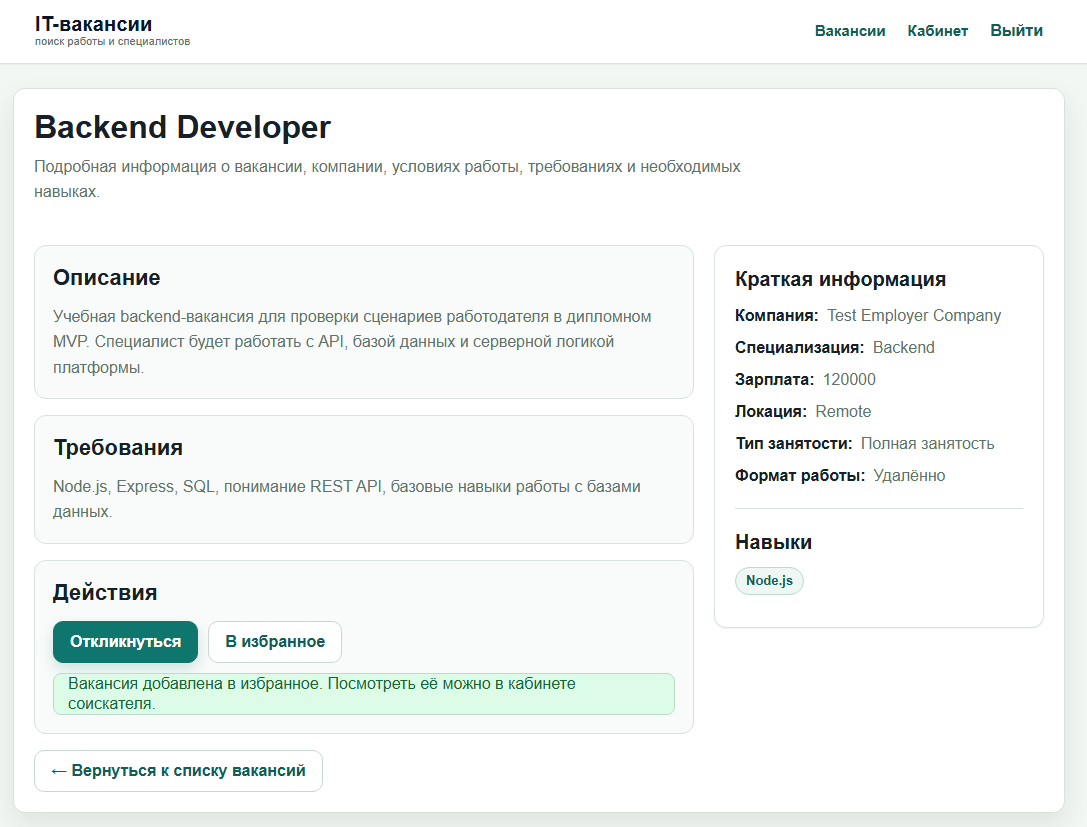
\includegraphics[width=1\linewidth]{tc06_favorites.png}}
	\caption{Результат добавления вакансии в избранное}
	\label{tc06:image}
\end{figure}

\subsubsection{TC-07. Создание и редактирование компании}

Цель тест-кейса: проверить возможность создания и редактирования профиля компании работодателем.

Предусловие: пользователь зарегистрирован с ролью работодателя и выполнил вход в систему.

Шаги выполнения тест-кейса:
\begin{enumerate}
	\item Открыть личный кабинет работодателя.
	\item Перейти на страницу управления компанией.
	\item Заполнить название компании, описание и адрес сайта.
	\item Сохранить данные компании.
	\item Изменить одно или несколько полей компании.
	\item Повторно сохранить изменения.
\end{enumerate}

Ожидаемый результат: система создаёт профиль компании, связывает его с текущим работодателем и позволяет владельцу компании редактировать её данные.

Фактический результат: профиль компании был создан и связан с учётной записью текущего работодателя. После редактирования изменённые сведения о названии, описании или сайте компании сохранились и отобразились в интерфейсе работодателя. Тест-кейс пройден.

\subsubsection{TC-08. Создание и публикация вакансии}

Цель тест-кейса: проверить возможность создания вакансии работодателем и её последующей публикации.

Предусловие: пользователь зарегистрирован с ролью работодателя, выполнил вход в систему и имеет созданный профиль компании.

Шаги выполнения тест-кейса:
\begin{enumerate}
	\item Открыть личный кабинет работодателя.
	\item Перейти на страницу управления вакансиями.
	\item Создать новую вакансию, заполнив название, специализацию, описание, требования, тип занятости и формат работы.
	\item Сохранить вакансию.
	\item Выполнить публикацию созданной вакансии.
	\item Перейти на страницу списка опубликованных вакансий.
	\item Проверить наличие опубликованной вакансии в общем списке.
\end{enumerate}

Ожидаемый результат: система создаёт вакансию, связывает её с компанией работодателя, переводит вакансию в опубликованный статус и отображает её в общем списке вакансий.

Фактический результат: вакансия была создана от имени компании текущего работодателя, после публикации получила статус опубликованной и стала доступна в общем списке вакансий для просмотра пользователями платформы. Тест-кейс пройден.

На рисунке \ref{tc08:image} представлен результат публикации вакансии работодателем.

\begin{figure}[H]
	\center{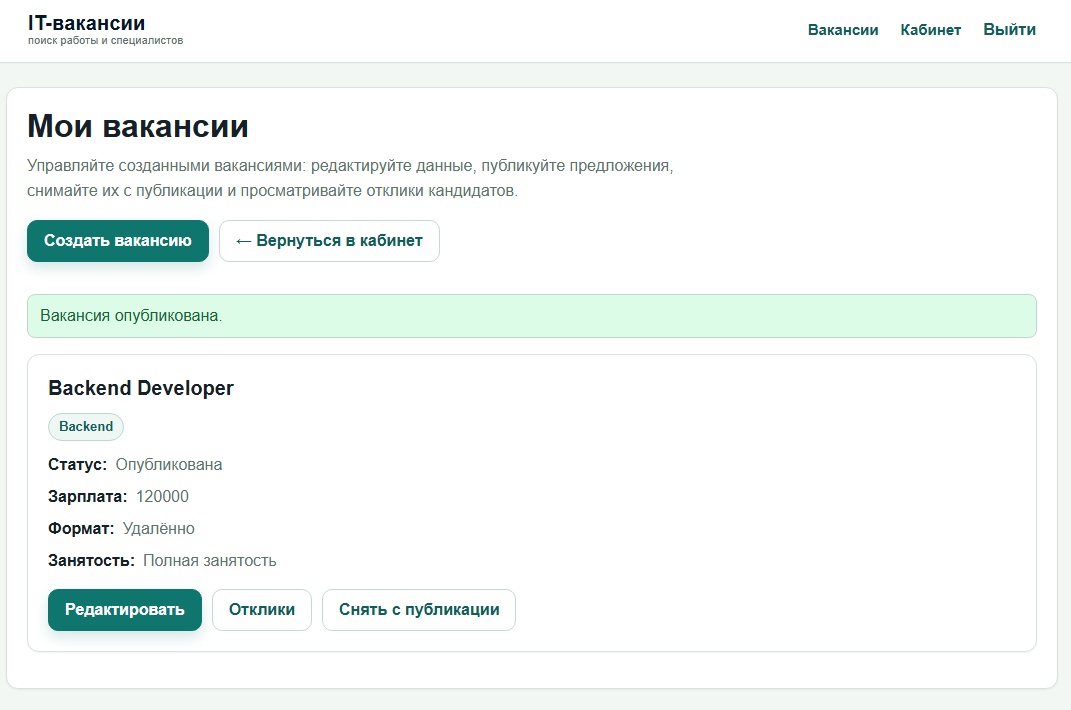
\includegraphics[width=1\linewidth]{tc08_publish_vacancy.png}}
	\caption{Результат публикации вакансии работодателем}
	\label{tc08:image}
\end{figure}

\subsubsection{TC-09. Просмотр откликов работодателем}

Цель тест-кейса: проверить возможность просмотра работодателем откликов, поступивших на принадлежащую ему вакансию.

Предусловие: пользователь зарегистрирован с ролью работодателя, выполнил вход в систему, имеет созданную компанию и опубликованную вакансию. В системе существует отклик соискателя на данную вакансию.

Шаги выполнения тест-кейса:
\begin{enumerate}
	\item Открыть личный кабинет работодателя.
	\item Перейти на страницу управления вакансиями.
	\item Выбрать опубликованную вакансию, на которую был отправлен отклик.
	\item Открыть список откликов по выбранной вакансии.
	\item Проверить отображение сведений о соискателе и статусе отклика.
\end{enumerate}

Ожидаемый результат: система отображает список откликов, связанных с выбранной вакансией работодателя, включая сведения о соискателях и текущие статусы откликов.

Фактический результат: после открытия списка откликов работодатель увидел заявки, связанные с выбранной вакансией. В интерфейсе отобразились сведения о соискателях, их профилях и текущих статусах откликов. Тест-кейс пройден.

На рисунке \ref{tc09:image} представлен список откликов, поступивших на вакансию работодателя.

\begin{figure}[H]
	\center{
\includegraphics[width=1\linewidth]{tc09_employer_applications.png}}
	\caption{Список откликов на вакансию работодателя}
	\label{tc09:image}
\end{figure}

\subsubsection{TC-10. Изменение статуса отклика}

Цель тест-кейса: проверить возможность изменения работодателем статуса отклика на принадлежащую ему вакансию.

Предусловие: пользователь зарегистрирован с ролью работодателя, выполнил вход в систему, имеет опубликованную вакансию и полученный отклик от соискателя.

Шаги выполнения тест-кейса:
\begin{enumerate}
	\item Открыть личный кабинет работодателя.
	\item Перейти к списку откликов на выбранную вакансию.
	\item Выбрать отклик соискателя.
	\item Изменить статус отклика, например на \texttt{in\_review}, \texttt{accepted} или \texttt{rejected}.
	\item Сохранить изменение статуса.
	\item Проверить, что новый статус отображается в интерфейсе работодателя и в списке откликов соискателя.
\end{enumerate}

Ожидаемый результат: система изменяет статус выбранного отклика и сохраняет новое значение в базе данных.

Фактический результат: выбранный отклик получил новый статус, изменение сохранилось в системе и отобразилось в интерфейсе работодателя. Обновлённый статус также стал доступен соискателю в списке его откликов. Тест-кейс пройден.

На рисунке \ref{tc10:image} представлен результат изменения статуса отклика работодателем.

\begin{figure}[H]
	\center{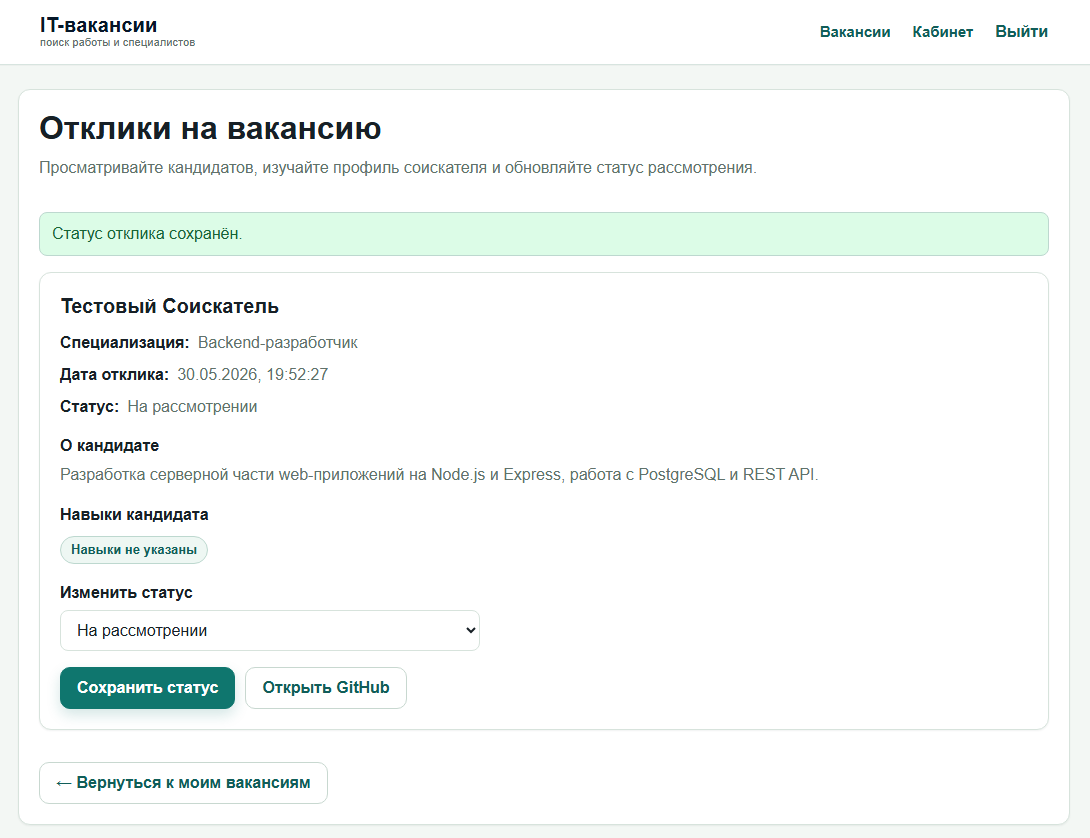
\includegraphics[width=1\linewidth]{tc10_application_status.png}}
	\caption{Результат изменения статуса отклика}
	\label{tc10:image}
\end{figure}

\subsubsection{TC-11. Поиск и фильтрация кандидатов}

Цель тест-кейса: проверить возможность поиска и фильтрации профилей соискателей работодателем.

Предусловие: пользователь зарегистрирован с ролью работодателя, выполнил вход в систему, в системе существуют профили соискателей с заполненной специализацией и навыками.

Шаги выполнения тест-кейса:
\begin{enumerate}
	\item Открыть личный кабинет работодателя.
	\item Перейти на страницу поиска кандидатов.
	\item Ввести значение специализации или выбрать навык для фильтрации.
	\item Применить параметры поиска.
	\item Открыть профиль одного из найденных соискателей.
\end{enumerate}

Ожидаемый результат: система отображает список профилей соискателей, соответствующих заданным параметрам поиска и фильтрации, а также позволяет открыть подробную информацию о выбранном кандидате.

Фактический результат: после применения параметров поиска список кандидатов обновился, и в нём отобразились профили соискателей, соответствующие выбранной специализации или навыку. Профиль выбранного кандидата открылся и отобразил профессиональные сведения соискателя. Тест-кейс пройден.

На рисунке \ref{tc11:image} представлен результат поиска и фильтрации кандидатов работодателем.

\begin{figure}[H]
	\center{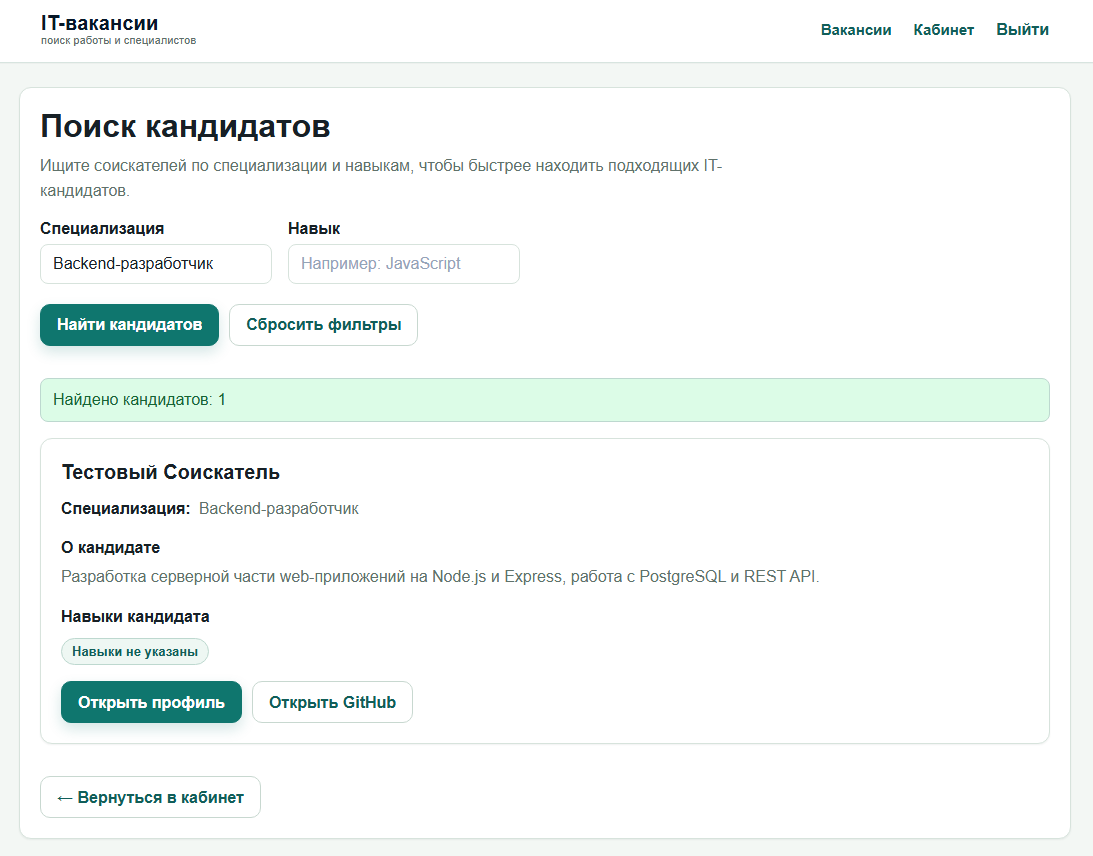
\includegraphics[width=1\linewidth]{tc11_candidate_search.png}}
	\caption{Результат поиска и фильтрации кандидатов}
	\label{tc11:image}
\end{figure}

\subsubsection{TC-12. Административное управление пользователями и вакансиями}

Цель тест-кейса: проверить возможность выполнения административных действий по управлению пользователями и вакансиями.

Предусловие: пользователь зарегистрирован с ролью администратора и выполнил вход в систему. В системе существуют зарегистрированные пользователи и созданные вакансии.

Шаги выполнения тест-кейса:
\begin{enumerate}
	\item Открыть личный кабинет администратора.
	\item Перейти на страницу управления пользователями.
	\item Проверить отображение списка пользователей.
	\item Выполнить блокировку выбранного пользователя.
	\item Перейти на страницу управления вакансиями.
	\item Проверить отображение списка вакансий.
	\item Выполнить удаление выбранной вакансии.
\end{enumerate}

Ожидаемый результат: система отображает списки пользователей и вакансий, позволяет администратору заблокировать пользователя и удалить выбранную вакансию.

Фактический результат: в административном интерфейсе отобразились списки пользователей и вакансий. После выполнения блокировки у выбранного пользователя был изменён признак доступа к системе, а выбранная вакансия была удалена из списка вакансий. Тест-кейс пройден.

На рисунке \ref{tc12:image} представлен интерфейс административного управления пользователями.

\begin{figure}[H]
	\center{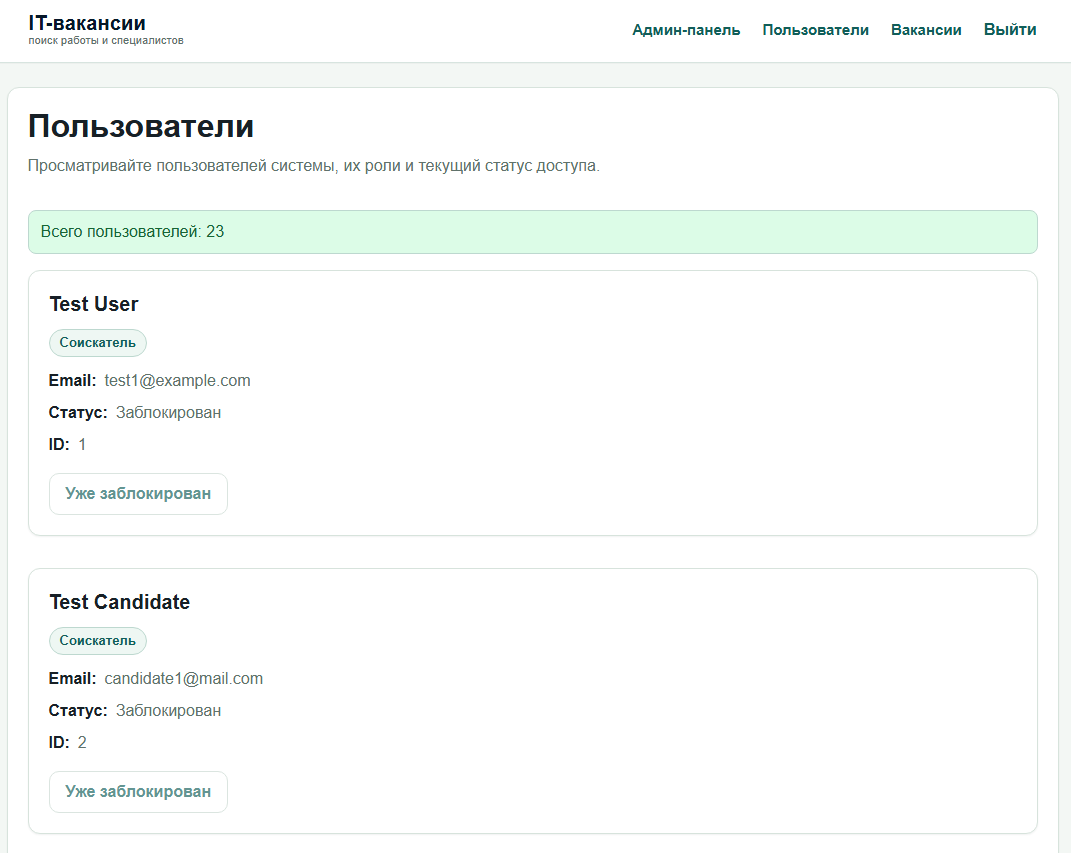
\includegraphics[width=1\linewidth]{tc12_admin_panel.png}}
	\caption{Интерфейс административного управления пользователями}
	\label{tc12:image}
\end{figure}

\subsubsection{TC-13. Проверка разграничения прав доступа}

Цель тест-кейса: проверить корректность ограничения доступа к функциям программной системы в зависимости от роли пользователя.

Предусловие: в системе существуют пользователи с ролями соискателя, работодателя и администратора.

Шаги выполнения тест-кейса:
\begin{enumerate}
	\item Открыть защищённую страницу без выполнения входа в систему.
	\item Проверить реакцию системы на попытку доступа без авторизации.
	\item Выполнить вход в систему под учётной записью соискателя.
	\item Попытаться открыть страницу управления компанией или вакансиями работодателя.
	\item Выполнить вход в систему под учётной записью работодателя.
	\item Попытаться открыть функции, предназначенные для соискателя, например управление избранными вакансиями.
	\item Выполнить вход в систему под обычной учётной записью и попытаться открыть административный раздел.
	\item Выполнить вход в систему под учётной записью администратора и проверить доступ к административным функциям.
\end{enumerate}

Ожидаемый результат: система запрещает доступ к защищённым страницам без авторизации, не позволяет пользователям выполнять действия, не соответствующие их роли, и предоставляет доступ к административным функциям только пользователю с ролью администратора.

Фактический результат: при попытке открыть защищённые страницы без авторизации система не предоставила доступ к закрытым функциям. Пользователи с ролями соискателя, работодателя и администратора получили доступ только к тем разделам, которые соответствуют их роли, а попытки обращения к недоступным функциям были заблокированы. Тест-кейс пройден.

На рисунке \ref{tc13:image} представлен результат попытки открытия защищённого раздела без авторизации.

\begin{figure}[H]
	\center{
\includegraphics[width=1\linewidth]{tc13_access_control.png}}
	\caption{Результат ограничения доступа к защищённому разделу}
	\label{tc13:image}
\end{figure}

\subsubsection{Нефункциональное тестирование}

Помимо проверки основных пользовательских сценариев было выполнено нефункциональное тестирование программной системы. Оно было направлено на проверку корректности работы интерфейса, обработки ошибочных ситуаций, ограничения доступа и устойчивости системы к некорректным действиям пользователя.

В ходе нефункционального тестирования проверялась работа защищённых страниц. При попытке открытия личного кабинета без авторизации система не предоставляла доступ к закрытым функциям и перенаправляла пользователя к странице входа. Также проверялись действия пользователей с разными ролями. Соискатель не получал доступ к функциям работодателя и администратора, работодатель не получал доступ к административным функциям, а административные действия были доступны только пользователю с соответствующей ролью.

Отдельно проверялась обработка некорректных данных. При отправке форм с незаполненными обязательными полями система не выполняла операцию и отображала сообщение об ошибке. Такая проверка выполнялась для форм регистрации, входа, создания профиля соискателя, создания компании и создания вакансии.

Также проверялись ограничения повторных действий. Система не позволяла повторно отправить отклик на одну и ту же вакансию и повторно добавить одну и ту же вакансию в избранное. При выполнении таких действий пользователь получал сообщение об ошибке, а данные в системе не дублировались.

Проверка интерфейса показала, что основные страницы web-платформы корректно отображают данные, полученные от серверной части: списки вакансий, карточки вакансий, профили соискателей, сведения о компаниях, отклики, избранные вакансии и административные списки. При успешном выполнении операций пользователь получает соответствующее уведомление, а при ошибке отображается сообщение с причиной невозможности выполнения действия.

Таким образом, нефункциональное тестирование подтвердило корректную обработку ошибок, работу ограничений доступа, отсутствие дублирования данных при повторных действиях и корректное взаимодействие клиентской части с серверным API.

\subsubsection{Вывод по результатам тестирования}

По результатам системного тестирования было подтверждено, что основные функции разработанной web-платформы работают корректно. Проверка охватила основные пользовательские сценарии для гостя, соискателя, работодателя и администратора.

В ходе тестирования было установлено, что пользователь может зарегистрироваться и выполнить вход в систему, соискатель может создать и редактировать профиль, выполнять поиск вакансий, отправлять отклики и добавлять вакансии в избранное. Работодатель может создать профиль компании, создавать и публиковать вакансии, просматривать отклики соискателей, изменять их статусы и выполнять поиск кандидатов. Администратор может просматривать пользователей и вакансии, блокировать пользователей и удалять вакансии.

Также была проверена корректность разграничения прав доступа. Пользователи получают доступ только к тем функциям, которые соответствуют их роли. Попытки обращения к защищённым страницам без авторизации или к функциям другой роли блокируются системой.

Нефункциональное тестирование подтвердило корректную обработку ошибочных ситуаций, запрет повторных действий, таких как повторный отклик на одну вакансию или повторное добавление вакансии в избранное, а также корректное отображение сообщений об ошибках в пользовательском интерфейсе.

Таким образом, результаты тестирования подтверждают, что разработанная программная система реализует заявленные функциональные возможности и соответствует основным требованиям, сформулированным в техническом задании.

   \section*{ЗАКЛЮЧЕНИЕ}
\addcontentsline{toc}{section}{ЗАКЛЮЧЕНИЕ}

Итогом выпускной квалификационной работы стала онлайн-платформа с базой данных, предназначенная для поиска работы и подбора IT-специалистов. Основное внимание при разработке уделялось базовому циклу взаимодействия между соискателем и работодателем: публикации вакансий, поиску предложений, отправке откликов и обработке заявок.

Первая глава посвящена предметной области IT-рекрутинга. В ней отмечены особенности подбора IT-специалистов: значимость специализации, конкретных навыков, формата занятости и прозрачности статуса отклика. В этом же разделе выделены основные роли пользователей: гость, соискатель, работодатель и администратор. Проведённый анализ показал, что для решения выявленных проблем требуется единая web-платформа, объединяющая вакансии, профили кандидатов, отклики и средства административного контроля.

В техническом задании закреплены требования к системе: состав хранимых данных, функции для каждой роли, требования к интерфейсу, надёжности, информационной безопасности и совместимости. Варианты использования, описанные в этом разделе, охватывают основные сценарии взаимодействия пользователей с платформой.

Технический проект определил архитектуру приложения. Серверная часть построена на Node.js и Express, данные хранятся в PostgreSQL, для работы с базой данных используется Sequelize ORM. Клиентская часть реализована на HTML, CSS и JavaScript. Также спроектирована схема базы данных, в которую вошли таблицы пользователей, профилей соискателей, компаний, вакансий, откликов, избранных вакансий и навыков.

В процессе реализации созданы ключевые программные компоненты: регистрация и авторизация, профиль соискателя, компании работодателей, публикация и фильтрация вакансий, отклики, избранное, навыки, административное управление. Доступ к функциям разграничен по ролям: каждый пользователь получает только те возможности, которые соответствуют его роли.

Платформа реализует основные сценарии для каждой роли. Соискатель регистрируется, заполняет профиль с профессиональными сведениями, ищет вакансии, откликается и добавляет предложения в избранное. Работодатель создаёт компанию, публикует вакансии, просматривает отклики, меняет их статус и ищет кандидатов. Администратор контролирует пользователей и вакансии: может блокировать учётные записи и удалять некорректные предложения.

Системное тестирование охватило основные сценарии: регистрацию, вход, работу с профилем соискателя, поиск и фильтрацию вакансий, отклики, избранное, создание компании, публикацию вакансии, просмотр и изменение статусов откликов, поиск кандидатов, администрирование и проверку прав доступа. Результаты тестирования показали корректную работу проверенных функций.

Отдельно проверена обработка ошибок и ограничений. Без авторизации закрытые разделы недоступны, действия ограничены ролью пользователя, повторный отклик на одну вакансию или дублирование вакансии в избранном не выполняются. Это подтверждает выполнение требований по надёжности и информационной безопасности, заложенных в техническом задании.

Поставленная цель ВКР достигнута. Создана web-платформа, хранящая и обрабатывающая данные пользователей, профилей, компаний, вакансий, откликов, избранного и навыков, а также поддерживающая ключевые процессы поиска работы и подбора IT-специалистов.

В дальнейшем систему можно развивать. Среди возможных направлений: уведомления, восстановление пароля, загрузка PDF-резюме, расширенная модерация, личные сообщения, а также рекомендательные механизмы для подбора вакансий и кандидатов. 

}\fi
\clearpage
\addcontentsline{toc}{section}{СПИСОК ИСПОЛЬЗОВАННЫХ ИСТОЧНИКОВ}

\begin{thebibliography}{99}
	
	\bibitem{sequelize_docs}
	Sequelize Documentation : [сайт]. – URL: https://sequelize.org/docs/v6/ (дата обращения: 13.05.2026).
	
	\bibitem{sequelize_getting_started}
	Getting Started // Sequelize Documentation : [сайт]. – URL: https://sequelize.org/docs/v6/getting-started/ (дата обращения: 13.05.2026).
	
	\bibitem{sequelize_model_basics}
	Model Basics // Sequelize Documentation : [сайт]. – URL: https://sequelize.org/docs/v6/core-concepts/model-basics/ (дата обращения: 13.05.2026).
	
	\bibitem{sequelize_associations}
	Associations // Sequelize Documentation : [сайт]. – URL: https://sequelize.org/docs/v6/core-concepts/assocs/ (дата обращения: 13.05.2026).
	
	\bibitem{rfc7519}
	Jones, M. JSON Web Token (JWT) / M. Jones, J. Bradley, N. Sakimura. – RFC~7519. – 2015. – URL: https://www.rfc-editor.org/rfc/rfc7519.html (дата обращения: 13.05.2026).
	
	\bibitem{rfc6265}
	Barth, A. HTTP State Management Mechanism / A. Barth. – RFC~6265. – 2011. – URL: https://www.rfc-editor.org/rfc/rfc6265.html (дата обращения: 13.05.2026).
	
	\bibitem{jsonwebtoken_npm}
	jsonwebtoken // npm : [сайт]. – URL: https://www.npmjs.com/package/jsonwebtoken (дата обращения: 13.05.2026).
	
	\bibitem{bcryptjs_npm}
	bcryptjs // npm : [сайт]. – URL: https://www.npmjs.com/package/bcryptjs (дата обращения: 13.05.2026).
	
	\bibitem{docker_compose_docs}
	Docker Compose // Docker Documentation : [сайт]. – URL: https://docs.docker.com/compose/ (дата обращения: 13.05.2026).
	
	\bibitem{compose_file_reference}
	Compose file reference // Docker Documentation : [сайт]. – URL: https://docs.docker.com/reference/compose-file/ (дата обращения: 13.05.2026).
	
	\bibitem{express_routing}
	Express routing // Express : [сайт]. – URL: https://expressjs.com/en/guide/routing.html (дата обращения: 13.05.2026).
	
	\bibitem{express_static_files}
	Serving static files in Express // Express : [сайт]. – URL: https://expressjs.com/en/starter/static-files.html (дата обращения: 13.05.2026).
	
	\bibitem{node_process_docs}
	Process // Node.js Documentation : [сайт]. – URL: https://nodejs.org/api/process.html (дата обращения: 13.05.2026).
	
	\bibitem{cookie_parser_npm}
	cookie-parser // npm : [сайт]. – URL: https://www.npmjs.com/package/cookie-parser (дата обращения: 13.05.2026).
	
	\bibitem{cors_npm}
	cors // npm : [сайт]. – URL: https://www.npmjs.com/package/cors (дата обращения: 13.05.2026).
	
	\bibitem{freeman_js}
	Фримен, А. Практикум по программированию на JavaScript / А. Фримен. – Москва~: Вильямс, 2013. – 960~с. – ISBN 978-5-8459-1799-7. – Текст~: непосредственный.
	
	\bibitem{crockford_js}
	Крокфорд, Д. JavaScript: сильные стороны / Д. Крокфорд. – Санкт-Петербург~: Питер, 2012. – 176~с. – ISBN 978-5-459-00788-6. – Текст~: непосредственный.
	
	\bibitem{haverbeke_js}
	Хавербеке, М. Выразительный JavaScript / М. Хавербеке. – Санкт-Петербург~: Питер, 2019. – 472~с. – ISBN 978-5-4461-1211-1. – Текст~: непосредственный.
	
	\bibitem{cantelon_node}
	Кантелон, М. Node.js в действии / М. Кантелон, М. Хартил, Т. Холовейчук, Н. Раджлич. – Санкт-Петербург~: Питер, 2014. – 416~с. – ISBN 978-5-496-00968-3. – Текст~: непосредственный.
	
	\bibitem{casciaro_node}
	Касчиаро, М. Node.js. Шаблоны проектирования / М. Касчиаро, Л. Маммино. – Санкт-Петербург~: Питер, 2021. – 672~с. – ISBN 978-5-4461-1668-3. – Текст~: непосредственный.
	
	\bibitem{obe_postgresql}
	Обе, Р. PostgreSQL: основы языка SQL / Р. Обе, Л. Хсу. – Санкт-Петербург~: БХВ-Петербург, 2016. – 336~с. – ISBN 978-5-9775-3589-2. – Текст~: непосредственный.
	
	\bibitem{slotin_postgresql}
	Слотин, Г. PostgreSQL~11. Мастерство разработки / Г. Слотин. – Москва~: ДМК Пресс, 2019. – 562~с. – ISBN 978-5-97060-759-6. – Текст~: непосредственный.
	
	\bibitem{date_db}
	Дейт, К.~Дж. Введение в системы баз данных / К.~Дж. Дейт. – Москва~: Вильямс, 2005. – 1328~с. – ISBN 5-8459-0788-8. – Текст~: непосредственный.
	
	\bibitem{karwin_sql}
	Карвин, Б. SQL. Антипаттерны программирования / Б. Карвин. – Санкт-Петербург~: Питер, 2011. – 304~с. – ISBN 978-5-459-00723-7. – Текст~: непосредственный.
	
	\bibitem{duckett_html_css}
	Дэкетт, Д. HTML и CSS. Разработка и создание веб-сайтов / Д. Дэкетт. – Москва~: Эксмо, 2014. – 480~с. – ISBN 978-5-699-64193-2. – Текст~: непосредственный.
	
	\bibitem{goldstein_html5}
	Голдстайн, А. HTML5 и CSS3 для всех / А. Голдстайн, Л. Лазарис, Э. Уэйл. – Москва~: Вильямс, 2012. – 368~с. – ISBN 978-5-699-57580-0. – Текст~: непосредственный.
	
	\bibitem{duckett_js_jquery}
	Дэкетт, Д. JavaScript и jQuery. Интерактивная web-разработка / Д. Дэкетт. – Москва~: Эксмо, 2017. – 640~с. – ISBN 978-5-699-80285-2. – Текст~: непосредственный.
	
	\bibitem{freyn_html5_css3}
	Фрейн, Б. HTML5 и CSS3. Разработка современных web-сайтов / Б. Фрейн. – 2-е изд. – Санкт-Петербург~: Питер, 2022. – 384~с. – ISBN 978-5-4461-0526-2. – Текст~: непосредственный.
	
	\bibitem{vero_css}
	Веру, Л. Секреты CSS. Идеальные решения ежедневных задач / Л. Веру. – Санкт-Петербург~: Питер, 2016. – 336~с. – ISBN 978-5-496-02082-4. – Текст~: непосредственный.
	
	\bibitem{macfarland_css}
	Макфарланд, Д. Большая книга CSS / Д. Макфарланд. – Санкт-Петербург~: Питер, 2012. – 560~с. – ISBN 978-5-496-02080-0. – Текст~: непосредственный.
	
	\bibitem{lawson_html5}
	Лоусон, Б. Изучаем HTML5. Библиотека специалиста / Б. Лоусон, Р. Шарп. – Санкт-Петербург~: Питер, 2013. – 286~с. – ISBN 978-5-459-01156-2. – Текст~: непосредственный.
	
	\bibitem{connolly_db}
	Коннолли, Т. Базы данных. Проектирование, реализация и сопровождение. Теория и практика / Т. Коннолли, К. Бегг. – 3-е изд. – Москва~: Вильямс, 2003. – 1440~с. – ISBN 978-5-8459-0527-7. – Текст~: непосредственный.
	
	\bibitem{groff_sql}
	Грофф, Дж.~Р. SQL: полное руководство / Дж.~Р. Грофф, П.~Н. Вайнберг, Э.~Дж. Оппель. – 3-е изд. – Санкт-Петербург~: Диалектика, 2020. – 960~с. – ISBN 978-5-907144-26-5. – Текст~: непосредственный.
	
	\bibitem{morgunov_postgresql}
	Моргунов, Е.~П. PostgreSQL. Основы языка SQL / Е.~П. Моргунов. – Санкт-Петербург~: БХВ-Петербург, 2022. – 336~с. – ISBN 978-5-9775-3960-9. – Текст~: непосредственный.
	
	\bibitem{chen_er}
	Чен, П. Модель «сущность-связь» – шаг к единому представлению данных / П. Чен. – Москва~: Мир, 1983. – Текст~: непосредственный.
	
	\bibitem{kent_nf}
	Кент, У. Простое руководство по пяти нормальным формам в теории реляционных баз данных / У. Кент. – Москва~: Мир, 1989. – Текст~: непосредственный.
	
	\bibitem{harder_transactions}
	Хардер, Т. Принципы транзакционной обработки баз данных / Т. Хардер, А. Ройтер. – Текст~: непосредственный // Системы управления базами данных. – 2004. – №~2. – С.~56--71.
	
	\bibitem{gandhi_git}
	Ганди, Р. Head First. Git / Р. Ганди. – Санкт-Петербург~: БХВ-Петербург, 2023. – 464~с. – ISBN 978-5-9775-1777-5. – Текст~: непосредственный.
	
	\bibitem{git_docs}
	Git Documentation : [сайт]. – URL: https://git-scm.com/doc (дата обращения: 24.04.2026).
	
	\bibitem{html_mdn}
	HTML // MDN Web Docs : [сайт]. – URL: https://developer.mozilla.org/ru/docs/Web/HTML (дата обращения: 24.04.2026).
	
	\bibitem{css_mdn}
	CSS // MDN Web Docs : [сайт]. – URL: https://developer.mozilla.org/ru/docs/Web/CSS (дата обращения: 24.04.2026).
	
	\bibitem{javascript_mdn}
	JavaScript // MDN Web Docs : [сайт]. – URL: https://developer.mozilla.org/ru/docs/Web/JavaScript (дата обращения: 24.04.2026).
	
	\bibitem{http_mdn}
	HTTP // MDN Web Docs : [сайт]. – URL: https://developer.mozilla.org/ru/docs/Web/HTTP (дата обращения: 24.04.2026).
	
	\bibitem{rfc9110}
	Fielding, R. HTTP Semantics / R. Fielding, M. Nottingham, J. Reschke. – RFC~9110. – 2022. – URL: https://www.rfc-editor.org/rfc/rfc9110.html (дата обращения: 24.04.2026).
	
	\bibitem{fielding_rest}
	Филдинг, Р. Архитектурный стиль REST и проектирование сетевых приложений : [сайт]. – URL: https://www.ics.uci.edu/~fielding/pubs/dissertation/rest\_arch\_style.htm (дата обращения: 24.04.2026).
	
	\bibitem{postgresql_docs}
	PostgreSQL Documentation : [сайт]. – URL: https://www.postgresql.org/docs/ (дата обращения: 24.04.2026).
	
	\bibitem{nodejs_docs}
	Node.js Documentation : [сайт]. – URL: https://nodejs.org/docs/latest/api/ (дата обращения: 11.05.2026).
	
	\bibitem{npm_docs}
	npm Docs : [сайт]. – URL: https://docs.npmjs.com/ (дата обращения: 11.05.2026).
	
	\bibitem{express_api}
	Express 4.x API Reference // Express : [сайт]. – URL: https://expressjs.com/en/4x/api.html (дата обращения: 11.05.2026).
	
	\bibitem{docker_docs}
	Docker Documentation : [сайт]. – URL: https://docs.docker.com/ (дата обращения: 24.04.2026).
	
	\bibitem{json_mdn}
	JSON // MDN Web Docs : [сайт]. – URL: https://developer.mozilla.org/docs/Glossary/JSON (дата обращения: 11.05.2026).
	
	\bibitem{fetch_api_mdn}
	Fetch API // MDN Web Docs : [сайт]. – URL: https://developer.mozilla.org/docs/Web/API/Fetch\_API (дата обращения: 11.05.2026).
	
	\bibitem{dom_mdn}
	Document Object Model (DOM) // MDN Web Docs : [сайт]. – URL: https://developer.mozilla.org/docs/Web/API/Document\_Object\_Model (дата обращения: 11.05.2026).
	
\end{thebibliography}

\ifВКР{\appendix{Представление графического материала}

Графический материал, выполненный на отдельных листах,
изображен на рисунках А.1--А.\arabic{числоПлакатов}.
\setcounter{числоПлакатов}{0}

\renewcommand{\thefigure}{А.\arabic{figure}} % шаблон номера для плакатов

\begin{landscape}

\begin{плакат}
	
\includegraphics[width=0.82\linewidth]{Plakat_01_Svedeniya_o_VKRB.pdf}
	\заголовок{Сведения о ВКРБ}
	\label{pl1:image}
\end{плакат}

\begin{плакат}
	
\includegraphics[width=0.82\linewidth]{Plakat_02_Cel_i_zadachi_razrabotki.pdf}
	\заголовок{Цель и задачи разработки}
	\label{pl2:image}
\end{плакат}

\begin{плакат}
	\includegraphics[width=0.82\linewidth]{Plakat_03_Diagramma_precedentov.png}
	\заголовок{Диаграмма прецедентов. Часть 1}
	\label{pl3:image}
\end{плакат}

\begin{плакат}
	\includegraphics[width=0.82\linewidth]{Plakat_04_Diagramma_precedentov2.png}
	\заголовок{Диаграмма прецедентов. Часть 2}
	\label{pl4:image}
\end{плакат}

\begin{плакат}
	
\includegraphics[width=0.82\linewidth]{Plakat_05_Arhitektura_programmnoi_sistemy.pdf}
	\заголовок{Архитектура системы}
	\label{pl5:image}
\end{плакат}

\begin{плакат}
	
\includegraphics[width=0.82\linewidth]{Plakat_06_ER_model_bazy_dannyh.pdf}
	\заголовок{ER-диаграмма}
	\label{pl6:image}
\end{плакат}

\begin{плакат}
	
\includegraphics[width=0.82\linewidth]{Plakat_07_Zaklyuchenie.pdf}
	\заголовок{Заключение}
	\label{pl7:image}
\end{плакат}


\end{landscape}
}\fi
\ifПрактика{}\else{\appendix{Фрагменты исходного кода программы}

\textbf{Листинг Б.1 -- Настройка серверного приложения}
\lstinputlisting[style=jslisting]{listings/server.js}

\textbf{Листинг Б.2 -- Подключение API-маршрутов программной системы}
\lstinputlisting[style=jslisting]{listings/index.js}

\textbf{Листинг Б.3 -- Реализация регистрации и авторизации пользователей}
\lstinputlisting[style=jslisting]{listings/auth.service.js}

\textbf{Листинг Б.4 -- Формирование JWT-токена и управление сессией пользователя}
\lstinputlisting[style=jslisting]{listings/auth.controller.js}

\textbf{Листинг Б.5 -- Проверка JWT-токена пользователя}
\lstinputlisting[style=jslisting]{listings/auth.middleware.js}

\textbf{Листинг Б.6 -- Разграничение доступа пользователей по ролям}
\lstinputlisting[style=jslisting]{listings/role.middleware.js}

\textbf{Листинг Б.7 -- Маршруты работы с вакансиями}
\lstinputlisting[style=jslisting]{listings/vacancy.routes.js}

\textbf{Листинг Б.8 -- Контроллер обработки запросов к вакансиям}
\lstinputlisting[style=jslisting]{listings/vacancy.controller.js}

\textbf{Листинг Б.9 -- Реализация отправки и обработки откликов}
\lstinputlisting[style=jslisting]{listings/application.service.js}

\textbf{Листинг Б.10 -- Реализация административных функций}
\lstinputlisting[style=jslisting]{listings/admin.service.js}

\ifВКР{
	\newpage
	\addcontentsline{toc}{section}{На отдельных листах (CD-RW в прикрепленном конверте)}
	\noindent
	\begin{tabular}{p{5.8cm}C{4.8cm}C{4.8cm}}
		Автор ВКР & \lhrulefill{\fill} & \fillcenter\Автор \\
		\setarstrut{\footnotesize}
		& \footnotesize{(подпись, дата)} & \\
		\restorearstrut
		Руководитель ВКР & \lhrulefill{\fill} & \fillcenter\Руководитель \\
		\setarstrut{\footnotesize}
		& \footnotesize{(подпись, дата)} & \\
		\restorearstrut
		Нормоконтроль & \lhrulefill{\fill} & \fillcenter\Нормоконтроль \\
		\setarstrut{\footnotesize}
		& \footnotesize{(подпись, дата)} & \\
		\restorearstrut
	\end{tabular}
	\vskip 2cm
	\begin{center}
		\textbf{Место для диска}
	\end{center}
}\fi}\fi
\end{document}
